% !TeX program = xelatex
% !TeX root = main.tex
% Cấu trúc và bố cục dựa trên mẫu local_docs/Report/.
% !TeX program = xelatex
% !TeX root = ../main.tex
% Preamble tập trung theo cấu trúc mẫu local_docs/Report/Sections/preamp.tex.
% Dùng XeLaTeX để giữ Unicode tiếng Việt trong nội dung và mã nguồn.
\documentclass[a4paper,oneside]{article}
\usepackage{fix-cm}
\usepackage{fontspec}
% Latin Modern giữ dáng Computer Modern/VNR của mẫu, hỗ trợ Unicode tiếng Việt.
% Chỉ định file để máy local và Docker chọn cùng một bộ font.
\setmainfont{lmroman12-regular.otf}[
  BoldFont=lmroman12-bold.otf,ItalicFont=lmroman12-italic.otf,
  BoldItalicFont=lmroman10-bolditalic.otf]
\setmonofont{lmmono10-regular.otf}[
  BoldFont=lmmonolt10-bold.otf,ItalicFont=lmmono10-italic.otf,
  BoldItalicFont=lmmonolt10-boldoblique.otf]
\usepackage[a4paper,total={160mm,240mm},left=30mm,top=30mm,
  headheight=40pt,headsep=10pt,footskip=26pt]{geometry}
\usepackage{setspace,indentfirst}
\setlength{\parindent}{1cm}
\hyphenpenalty=10000
\exhyphenpenalty=10000
\emergencystretch=3em
\raggedbottom

\usepackage{amsmath,amssymb}
\usepackage{enumitem,graphicx,array,tabularx,multirow,booktabs,float}
\usepackage[table,dvipsnames]{xcolor}
\usepackage{caption,subcaption,listings,fvextra}
\usepackage{tikz,eso-pic}
\usetikzlibrary{calc,positioning,arrows.meta,shapes.geometric}
\usepackage{pgfplots}
\pgfplotsset{compat=1.18}
\usepackage{fancyhdr,titlesec}
\usepackage[backend=biber,style=ieee]{biblatex}
\addbibresource{references.bib}
\newif\ifreportcitations
\AtEveryCitekey{\global\reportcitationstrue}
\usepackage{xurl,hyperref}

\newcommand{\khoa}{KHOA KHOA HỌC VÀ KỸ THUẬT MÁY TÍNH}
\newcommand{\monhoc}{HỆ QUẢN TRỊ CƠ SỞ DỮ LIỆU}
\newcommand{\detai}{Oracle vs Redis}
\newcommand{\lop}{L01}
\newcommand{\nhom}{L01\_02}
\newcommand{\hocky}{261}
\newcommand{\giangvien}{Lê Thị Bảo Thu}
\newcommand{\sinhvien}{Đặng Hải Sơn}
\newcommand{\mssv}{2312955}

\newcolumntype{L}{>{\raggedright\arraybackslash}X}
\newcolumntype{P}[1]{>{\raggedright\arraybackslash}p{#1}}
% Kiểu chèn code dùng chung, được \input trong main.tex.
% Dùng: \begin{lstlisting}[language=OracleSQL, caption={...}, label={lst:cc-...}] ... \end{lstlisting}
% Ngôn ngữ có sẵn: OracleSQL, Redis, Lua, Java, Python, bash. Đoạn chỉ là văn bản thì dùng Verbatim (fvextra).
% Nền code xám ấm theo mystyle của mẫu; log xám theo RResultStyle.
% Bảng dùng nền trắng, header xám trung tính để in đen trắng vẫn rõ.
\definecolor{ReportInk}{HTML}{202020}
\definecolor{ReportAccent}{HTML}{303030}
\definecolor{ReportBorder}{HTML}{707070}
\definecolor{ReportTableHead}{HTML}{EAEAEA}
\definecolor{ReportCodeBg}{rgb}{0.95,0.95,0.92}
\definecolor{ReportLogBg}{rgb}{0.94,0.94,0.94}
\colorlet{codebg}{ReportCodeBg}
\definecolor{codecomment}{HTML}{356858}
\definecolor{codekeyword}{HTML}{6E287A}
\definecolor{codestring}{HTML}{943D24}
\definecolor{codenumber}{HTML}{686868}

\newcommand{\reporttablesetup}{%
  \setstretch{1}\fontsize{11}{13}\selectfont%
  \setlength{\tabcolsep}{5pt}%
  \setlength{\arrayrulewidth}{0.5pt}%
  \setlength{\extrarowheight}{2pt}%
  \renewcommand{\arraystretch}{1.15}%
  \arrayrulecolor{ReportBorder}%
}
\newcommand{\reportheader}[1]{\textbf{\color{ReportInk}#1}}
% Cho bộ dàn trang chọn điểm ngắt trước caption. Không kiểm tra pagegoal rồi
% ép newpage: pagegoal có thể còn giá trị cũ khi đoạn vừa sang trang mới.
% Khoảng co giãn và penalty giữ caption cùng đầu khối, khối dài vẫn ngắt được.
\newcommand{\reportblockspace}[1]{%
  \par\begingroup
  \vskip 0pt plus #1\relax
  \penalty -100
  \vskip 0pt plus -#1\relax
  \vskip #1\relax
  \penalty 9999
  \vskip -#1\relax
  \endgroup
}
\setlength{\intextsep}{9pt plus 2pt minus 2pt}
\setlength{\textfloatsep}{10pt plus 2pt minus 2pt}
\setlength{\floatsep}{9pt plus 2pt minus 2pt}
% Bảng và hình là float nguyên khối; có thể lấp phần trống bằng đoạn văn kế tiếp.
\renewcommand{\topfraction}{0.95}
\renewcommand{\bottomfraction}{0.85}
\renewcommand{\textfraction}{0.05}
\renewcommand{\floatpagefraction}{0.85}
\setcounter{topnumber}{3}
\setcounter{bottomnumber}{2}
\setcounter{totalnumber}{5}
\newcommand{\reportmonosize}{\fontsize{10}{12}\selectfont}
\fvset{fontsize=\reportmonosize,baselinestretch=1,breaklines=true,
  breakanywhere=true,frame=single,framerule=0.5pt,framesep=6pt,
  rulecolor=ReportBorder,fillcolor=ReportLogBg,backgroundcolor=ReportLogBg,
  formatcom=\color{ReportInk},xleftmargin=6pt,xrightmargin=6pt,
  listparameters={\setlength{\topsep}{4pt}\setlength{\partopsep}{0pt}}}

\lstdefinestyle{shopflash}{
  basicstyle=\ttfamily\linespread{1}\fontsize{10}{12}\selectfont,
  backgroundcolor=\color{codebg},
  commentstyle=\itshape\color{codecomment},
  keywordstyle=\bfseries\color{codekeyword},
  stringstyle=\color{codestring},
  numbers=left, numberstyle=\tiny\color{codenumber}, numbersep=6pt,
  frame=single, rulecolor=\color{ReportBorder},framesep=5pt,
  xleftmargin=16pt,xrightmargin=5pt,
  breaklines=true, columns=fullflexible, keepspaces=true,
  showstringspaces=false, upquote=true, tabsize=2,
  captionpos=t, aboveskip=5pt, belowskip=5pt
}
\lstset{style=shopflash}

% SQL của Oracle: thêm các từ khóa SQL chuẩn của listings chưa có.
\lstdefinelanguage{OracleSQL}[]{SQL}{
  sensitive=false,
  morekeywords={MERGE,USING,MATCHED,NOWAIT,SKIP,LOCKED,WAIT,SERIALIZABLE,ISOLATION,LEVEL,
    SAVEPOINT,RETURNING,FETCH,FIRST,ROWS,ONLY,OFFSET,NVL,COALESCE,SYSTIMESTAMP,IDENTITY,
    GENERATED,PURGE,EXPLAIN,PLAN,OVER,PARTITION,WITH,EXISTS},
  morecomment=[l]{--}
}

% Lệnh redis-cli.
\lstdefinelanguage{Redis}{
  sensitive=false,
  alsoletter={.},
  morekeywords={GET,SET,DEL,UNLINK,EXISTS,EXPIRE,TTL,INCR,DECR,INCRBY,DECRBY,
    HGET,HSET,HMGET,HGETALL,HDEL,HINCRBY,HEXISTS,ZADD,ZREM,ZRANGE,ZRANGEBYSCORE,
    MULTI,EXEC,DISCARD,WATCH,UNWATCH,EVAL,EVALSHA,SCRIPT,FCALL,FUNCTION,TIME,
    JSON.SET,JSON.GET,FT.CREATE,FT.SEARCH,FT.AGGREGATE,FT.PROFILE,FT.INFO,
    SCAN,INFO,CONFIG,BGSAVE,BGREWRITEAOF,FLUSHDB},
  morecomment=[l]{\#},
  morestring=[b]"
}

% Transaction report formatting. Loaded in the preamble; no extra packages.
\DeclareCaptionType{txresult}[Kết quả][Danh sách kết quả]
\captionsetup[txresult]{position=top,skip=5pt,hypcap=false}
\lstdefinelanguage{TransactionLua}{
  sensitive=true,
  morekeywords={and,break,do,else,elseif,end,false,for,function,if,in,local,nil,not,or,repeat,return,then,true,until,while},
  morecomment=[l]{--},
  morestring=[b]",
  morestring=[b]'
}
\lstdefinelanguage{TransactionJavaScript}{
  sensitive=true,
  morekeywords={const,let,var,function,return,if,else,for,while,new,true,false,null},
  morecomment=[l]{//},
  morecomment=[s]{/*}{*/},
  morestring=[b]",
  morestring=[b]'
}

% These definitions only take effect where \txnumbering is called.
\newcommand{\txnumbering}{%
  \setcounter{table}{0}%
  \setcounter{figure}{0}%
  \setcounter{lstlisting}{0}%
  \setcounter{txresult}{0}%
  \renewcommand{\thetable}{\thesubsection.\arabic{table}}%
  \renewcommand{\thefigure}{\thesubsection.\arabic{figure}}%
  \renewcommand{\thelstlisting}{\thesubsection.\arabic{lstlisting}}%
  \renewcommand{\thetxresult}{\thesubsection.\arabic{txresult}}%
  \renewcommand{\theHtable}{\thesubsection.\arabic{table}}%
  \renewcommand{\theHfigure}{\thesubsection.\arabic{figure}}%
  \renewcommand{\lstlistingname}{Mã nguồn}%
}

\graphicspath{{Pictures/}{Pictures/Task_4/}}

% Ba phần lớn; topic là subsection (2.1–2.6), nội dung Transaction đến cấp 4.
\setcounter{secnumdepth}{4}
\setcounter{tocdepth}{3}
\renewcommand{\thesection}{\arabic{section}}
\renewcommand{\thesubsection}{\arabic{section}.\arabic{subsection}}
\titleformat{\section}{\LARGE\bfseries}{Phần \thesection.}{0.7em}{}
\titleformat{\subsection}{\Large\bfseries}{\thesubsection}{1em}{}
\titleformat{\subsubsection}{\fontsize{14}{16}\selectfont\bfseries}{\thesubsubsection}{1em}{}
\renewcommand{\theparagraph}{\thesubsubsection.\arabic{paragraph}}
\titleformat{\paragraph}[block]{\fontsize{13}{15}\selectfont\bfseries}{\theparagraph}{0.7em}{}
\titlespacing*{\section}{0pt}{16pt}{9pt}
\titlespacing*{\subsection}{0pt}{12pt}{6pt}
\titlespacing*{\subsubsection}{0pt}{10pt}{5pt}
\titlespacing*{\paragraph}{0pt}{10pt}{5pt}
\counterwithin{table}{section}
\counterwithin{figure}{section}
\counterwithin{txresult}{section}
\renewcommand{\thetable}{\arabic{section}.\arabic{table}}
\renewcommand{\thefigure}{\arabic{section}.\arabic{figure}}
\renewcommand{\thetxresult}{\arabic{section}.\arabic{txresult}}
\AtBeginDocument{%
  \counterwithin{lstlisting}{section}%
  \renewcommand{\thelstlisting}{\arabic{section}.\arabic{lstlisting}}}
\renewcommand{\contentsname}{Mục lục}
\renewcommand{\figurename}{Hình}
\renewcommand{\tablename}{Bảng}
\renewcommand{\lstlistingname}{Mã nguồn}
\DeclareCaptionFont{reportcaption}{\fontsize{11}{13}\selectfont}
\captionsetup{font=reportcaption,labelfont=bf,textfont=it}
\captionsetup[table]{position=top,skip=5pt}
\captionsetup[figure]{position=bottom,skip=5pt}
\hypersetup{unicode=true,colorlinks=true,linkcolor=black,citecolor=black,
  urlcolor=ReportAccent,pdftitle={Oracle vs Redis -- Báo cáo Hệ quản trị Cơ sở dữ liệu},
  pdfauthor={Đặng Hải Sơn -- 2312955 -- L01 -- Nhóm \nhom}}

% Header/footer của mẫu, thay thông tin môn học và người thực hiện.
\pagestyle{fancy}
\fancyhf{}
\fancyhead[L]{%
  \begin{tabular}{rl}
    \begin{picture}(25,15)(0,0)
      \put(0,-8){
\includegraphics[width=8mm,height=8mm]{Pictures/hcmut.png}}
    \end{picture} &
    \begin{tabular}{l}
      \fontsize{10}{12}\selectfont\bfseries\ttfamily Trường Đại học Bách khoa -- ĐHQG-HCM\\
      \fontsize{10}{12}\selectfont\bfseries\ttfamily Khoa Khoa học và Kỹ thuật Máy tính
    \end{tabular}
  \end{tabular}}
\fancyfoot[L]{\footnotesize\ttfamily Báo cáo Hệ quản trị Cơ sở dữ liệu\\Học kỳ 261 -- Lớp L01 -- Nhóm \nhom}
\fancyfoot[R]{\footnotesize\ttfamily Trang {\color{red}\thepage/\pageref*{LastPage}}}
\renewcommand{\headrulewidth}{0.3pt}
\renewcommand{\footrulewidth}{0.3pt}

% Khung đôi bìa theo đúng cơ chế PageFrameSetup của template.
\pgfkeys{
  /pageframe/.is family,/pageframe,
  outer left/.initial=1.5cm,outer right/.initial=1.5cm,
  outer top/.initial=2cm,outer bottom/.initial=2cm,
  inner left/.initial=1.7cm,inner right/.initial=1.7cm,
  inner top/.initial=2.2cm,inner bottom/.initial=2.2cm,
  outer width/.initial=3pt,inner width/.initial=1.9pt,
  outer color/.initial=black,inner color/.initial=black,
  corner radius/.initial=0pt
}
\newcommand{\PageFrameSetup}[1]{\pgfkeys{/pageframe,#1}}
\newcommand{\PageFrameDraw}{%
  
\begin{tikzpicture}[overlay,remember picture]
    \draw[line width=\pgfkeysvalueof{/pageframe/outer width},
      color=\pgfkeysvalueof{/pageframe/outer color},
      rounded corners=\pgfkeysvalueof{/pageframe/corner radius}]
      ($(current page.north west)+(\pgfkeysvalueof{/pageframe/outer left},-\pgfkeysvalueof{/pageframe/outer top})$)
      rectangle
      ($(current page.south east)+(-\pgfkeysvalueof{/pageframe/outer right},\pgfkeysvalueof{/pageframe/outer bottom})$);
    \draw[line width=\pgfkeysvalueof{/pageframe/inner width},
      color=\pgfkeysvalueof{/pageframe/inner color},
      rounded corners=\pgfkeysvalueof{/pageframe/corner radius}]
      ($(current page.north west)+(\pgfkeysvalueof{/pageframe/inner left},-\pgfkeysvalueof{/pageframe/inner top})$)
      rectangle
      ($(current page.south east)+(-\pgfkeysvalueof{/pageframe/inner right},\pgfkeysvalueof{/pageframe/inner bottom})$);
  \end{tikzpicture}}
\newcommand{\PageFrameThisPage}{\AddToShipoutPictureBG*{\PageFrameDraw}}


\begin{document}
\pagenumbering{alph}
\begin{titlepage}
  \PageFrameSetup{
    outer left=1.5cm,outer right=1.5cm,outer top=2cm,outer bottom=2cm,
    inner left=1.7cm,inner right=1.7cm,inner top=2.2cm,inner bottom=2.2cm,
    outer width=3pt,inner width=1.9pt,
    outer color=black,inner color=black,corner radius=0pt
  }
  \thispagestyle{empty}
  \PageFrameThisPage
  \begin{center}
    {\Large ĐẠI HỌC QUỐC GIA THÀNH PHỐ HỒ CHÍ MINH}\\
    {\Large TRƯỜNG ĐẠI HỌC BÁCH KHOA}\\
    \textbf{\Large \khoa}
  \end{center}

  \vspace{0.5cm}
  \begin{figure}[h!]
    \centering
    
\includegraphics[scale=1]{Pictures/hcmut.png}
  \end{figure}
  \vspace{0.2cm}

  \begin{center}
    \textbf{\LARGE BÁO CÁO BÀI TẬP LỚN}\\[0.5cm]
    {\color{blue}\hrule}
    \vspace{0.5cm}
    {\color{blue}\textbf{\LARGE \detai}\\[0.5cm]}
    {\color{blue}\hrule}
    \vspace{0.5cm}

    \begin{table}[h]
      \large
      \centering
      \begin{tabular}{@{}r@{\hspace{1cm}}ll@{}}
        Môn học: & \monhoc & \\[0.25cm]
        Giảng viên hướng dẫn: & \giangvien & \\[0.25cm]
        Lớp: & \lop & \\[0.25cm]
        Nhóm: & \nhom & \\[0.25cm]
        Học kỳ: & \hocky & \\[0.25cm]
        Sinh viên thực hiện: & \sinhvien & \mssv
      \end{tabular}
    \end{table}
  \end{center}

  \vspace{0.6cm}
  \centering{\fontsize{12}{14}\selectfont THÀNH PHỐ HỒ CHÍ MINH -- 11/2026}
\end{titlepage}

\pagenumbering{arabic}
\setstretch{1.3}
{\fontsize{12}{15}\selectfont\tableofcontents\par}
\clearpage
\fontsize{13}{18}\selectfont
% !TeX root = ../main.tex
\section*{Danh sách thành viên và nhiệm vụ}
\addcontentsline{toc}{section}{Danh sách thành viên và nhiệm vụ}
\begin{table}[H]
\centering
\reporttablesetup
\begin{tabularx}{\linewidth}{|c|P{3cm}|P{2cm}|L|}
\hline
\rowcolor{ReportTableHead}
\reportheader{STT} & \reportheader{Họ và tên} & \reportheader{MSSV} & \reportheader{Nhiệm vụ} \\ \hline
1 & Đặng Hải Sơn & 2312955 & Transaction: nghiên cứu cơ chế Oracle và Redis, thực nghiệm ACID, đánh giá hiệu năng. \\ \hline
2 & Nguyễn Chí Duy Khang & 2311436 & Concurrency Control: nghiên cứu cơ chế Oracle và Redis, Concurrency Lab và thực nghiệm E1--E5; hiện thực chức năng Flash Sale (phía khách và quản trị). \\ \hline
\end{tabularx}
\end{table}


\clearpage
\section{GIỚI THIỆU ĐỀ TÀI VÀ TỔNG QUAN HỆ THỐNG}\label{sec:introduction}
\begingroup
\setstretch{1.15}
\fontsize{12}{16}\selectfont
% !TeX root = ../../main.tex
% Nội dung chuyển từ section_1.md ngày 17/11/2026; giữ nguyên văn.
% Hình kiến trúc dùng ảnh Pictures/image.png do người dùng cung cấp.
\subsection{Bối cảnh, mục tiêu và phạm vi đề tài}
Hệ quản trị cơ sở dữ liệu (DBMS) đóng vai trò quan trọng trong việc lưu trữ, truy xuất và bảo đảm tính toàn vẹn dữ liệu của các ứng dụng. Tuy nhiên, các hệ quản trị quan hệ (SQL) và phi quan hệ (NoSQL) có những khác biệt về mô hình dữ liệu, cơ chế xử lý và đặc tính hiệu năng, dẫn đến mức độ phù hợp khác nhau đối với từng loại nghiệp vụ.

Đề tài lựa chọn \textbf{Oracle Database và Redis} làm hai hệ quản trị đại diện để nghiên cứu, thực nghiệm và so sánh trên sáu chủ đề: Data Storage \& Management, Indexing, Query Processing, Transaction, Concurrency Control và Data Backup \& Recovery. Mục tiêu là làm rõ cơ chế hoạt động, đánh giá kết quả thực nghiệm và xác định cách sử dụng phù hợp của mỗi DBMS trong bối cảnh ứng dụng cụ thể.

Nhóm xây dựng \textbf{ShopFlash}, một ứng dụng thương mại điện tử có chức năng mua hàng thông thường và Flash Sale, làm bối cảnh nghiên cứu. Bên cạnh việc hiện thực các nghiệp vụ cơ bản, hệ thống còn hỗ trợ thực hiện và minh họa các thí nghiệm DBMS. Phạm vi triển khai và kiểm chứng tập trung vào môi trường local, không đặt mục tiêu xây dựng một nền tảng thương mại điện tử production hoàn chỉnh.

\subsection{Tổng quan ứng dụng ShopFlash}
ShopFlash là ứng dụng web mô phỏng hoạt động bán lẻ trực tuyến, cho phép người dùng tìm kiếm sản phẩm, quản lý giỏ hàng, đặt hàng và tham gia các chương trình Flash Sale. Hệ thống hỗ trợ khách truy cập, khách hàng có tài khoản và quản trị viên với các quyền truy cập tương ứng.

Hai luồng nghiệp vụ tiêu biểu của hệ thống gồm:

\begin{itemize}[leftmargin=1.3em,itemsep=2pt,topsep=3pt]
\item
\textbf{Normal Checkout:} Khách hàng lựa chọn sản phẩm, thêm vào giỏ hàng và thực hiện đặt hàng. Backend kiểm tra lại thông tin sản phẩm, giá và tồn kho trước khi tạo đơn, cập nhật tồn kho và giỏ hàng.

\item
\textbf{Flash Sale:} Khách hàng mua sản phẩm có số lượng giới hạn trong thời gian khuyến mãi. Hệ thống kiểm soát số suất còn lại, giới hạn mua theo người dùng và sử dụng reservation tạm thời trước khi xác nhận đơn hàng.

\end{itemize}

Ngoài các nghiệp vụ mua hàng, ShopFlash còn hỗ trợ quản lý danh mục, sản phẩm và báo cáo thống kê phục vụ hoạt động quản trị.

Các giao diện thực nghiệm về Storage, Indexing, Query Processing và Concurrency Control được xây dựng để hỗ trợ thao tác, quan sát kết quả và kiểm chứng các cơ chế DBMS. Đây là các công cụ phục vụ nghiên cứu, không phải những chức năng nghiệp vụ cốt lõi của hệ thống bán lẻ; nội dung thực nghiệm tương ứng được trình bày tại Phần 2.

\subsection{Kiến trúc hệ thống và phân chia dữ liệu Oracle–Redis}
ShopFlash được xây dựng theo kiến trúc web nhiều tầng, gồm Frontend, Backend và tầng dữ liệu sử dụng đồng thời Oracle Database và Redis.

\begin{itemize}[leftmargin=1.3em,itemsep=2pt,topsep=3pt]
\item
\textbf{Frontend:} Sử dụng React và Vite, cung cấp giao diện cho khách hàng, quản trị viên và các chức năng hỗ trợ thực nghiệm.

\item
\textbf{Backend:} Xây dựng bằng Java 21 và Spring Boot, cung cấp REST API, xử lý nghiệp vụ, xác thực người dùng và điều phối truy cập dữ liệu.

\item
\textbf{Tầng dữ liệu:} Oracle và Redis được vận hành trong Docker Compose. Backend kết nối Oracle thông qua JDBC và Redis thông qua Jedis.

\end{itemize}

Các module nghiệp vụ thuộc cùng một ứng dụng Backend, không được triển khai thành các microservice độc lập.

\paragraph*{Kiến trúc tổng thể}

\begin{figure}[H]
\centering
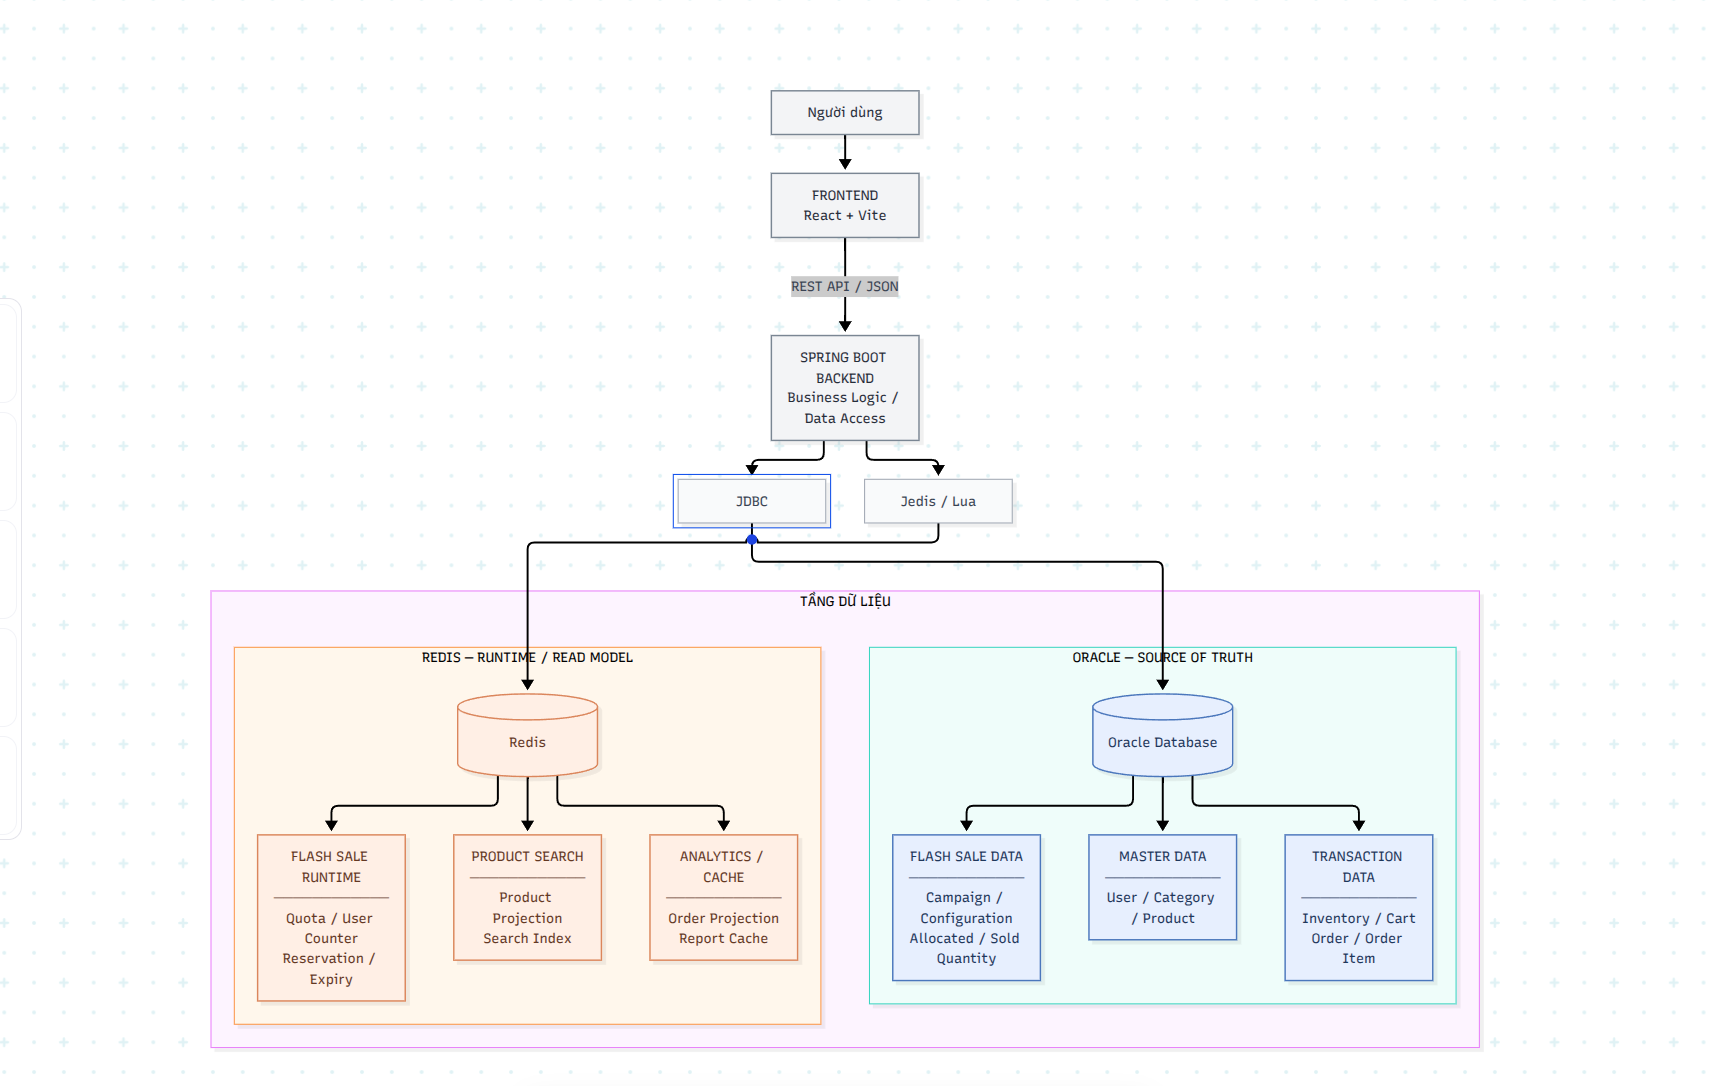
\includegraphics[width=\linewidth]{Pictures/image.png}
\caption{Kiến trúc tổng thể và vai trò của Oracle–Redis trong ShopFlash.}\label{fig:intro-architecture}
\end{figure}

\paragraph*{Phân chia trách nhiệm dữ liệu}

Hệ thống áp dụng nguyên tắc phân tách dữ liệu theo yêu cầu về tính nhất quán, khả năng lưu trữ và đặc điểm truy cập. Oracle giữ vai trò \emph{source of truth}, trong khi Redis đảm nhiệm các dữ liệu runtime hoặc dữ liệu dẫn xuất phục vụ những tác vụ phù hợp.

\begin{table}[H]
\centering
\caption{Phân chia trách nhiệm lưu trữ và xử lý dữ liệu giữa Oracle và Redis.}\label{tab:intro-data}
\reporttablesetup
\begin{tabularx}{\linewidth}{|>{\hsize=0.7\hsize\linewidth=\hsize}L|>{\hsize=1.15\hsize\linewidth=\hsize}L|>{\hsize=1.15\hsize\linewidth=\hsize}L|}
\hline
\rowcolor{ReportTableHead}
\reportheader{Nhóm dữ liệu} & \reportheader{Oracle Database} & \reportheader{Redis} \\ \hline
\textbf{Sản phẩm và tồn kho} & Lưu Product, Category, Inventory và trạng thái chính thức. & Lưu Product projection phục vụ tìm kiếm, lọc và hiển thị. \\ \hline
\textbf{Giỏ hàng và đơn hàng} & Quản lý Cart, Order, Order Items và các transaction đặt/hủy đơn. & Lưu dữ liệu dẫn xuất từ Order phục vụ thống kê và báo cáo. \\ \hline
\textbf{Flash Sale} & Lưu cấu hình chương trình, tồn kho phân bổ, số lượng bán và đơn hàng thành công. & Quản lý quota runtime, giới hạn mua theo người dùng và reservation tạm thời. \\ \hline
\textbf{Truy vấn và báo cáo} & Cung cấp dữ liệu nghiệp vụ gốc và các truy vấn quan hệ. & Hỗ trợ tìm kiếm, cache và analytics read model. \\ \hline
\end{tabularx}
\end{table}

\paragraph*{Cơ chế phối hợp giữa hai DBMS}

Trong \textbf{Normal Checkout}, các thao tác tạo Order, cập nhật Inventory và Cart được thực hiện trong Oracle transaction nhằm bảo đảm tính nhất quán của dữ liệu giao dịch.

Đối với \textbf{Flash Sale}, Redis xử lý bước kiểm tra và giữ quota tạm thời để đáp ứng các yêu cầu mua đồng thời. Sau đó, Oracle ghi nhận đơn hàng và cập nhật dữ liệu chính thức. Backend thực hiện xác nhận reservation hoặc bù trừ khi giao dịch không thành công; hai DBMS không sử dụng một distributed transaction chung.

Đối với \textbf{tìm kiếm và thống kê}, Redis lưu các bản dữ liệu dẫn xuất (\emph{projection}) được xây dựng từ Oracle nhằm tối ưu việc truy vấn mà không làm thay đổi nguồn dữ liệu chính thức. Product projection được cập nhật sau các thao tác quản lý sản phẩm liên quan, trong khi Analytics projection được tái tạo từ Oracle theo yêu cầu. Do các bản dữ liệu này được cập nhật riêng với giao dịch gốc, chúng có thể phản ánh thay đổi muộn hơn Oracle. Vì vậy, những nghiệp vụ cần xác nhận dữ liệu tại thời điểm xử lý, chẳng hạn kiểm tra giá và tồn kho khi Checkout, vẫn sử dụng trực tiếp dữ liệu Oracle.

Cách tổ chức này cho phép ShopFlash khai thác khả năng quản lý transaction và ràng buộc dữ liệu của Oracle, đồng thời sử dụng Redis cho những workload như tìm kiếm, truy vấn dữ liệu dẫn xuất và kiểm soát Flash Sale runtime. Đây cũng là cơ sở để nhóm triển khai các thí nghiệm so sánh hai DBMS trong Phần 2.

\par
\endgroup

\clearpage
\section{NGHIÊN CỨU VÀ SO SÁNH ORACLE VỚI REDIS}\label{sec:research}
% !TeX root = ../../main.tex
\subsection{Data Storage \& Management}\label{sec:storage}
\begingroup
% Đánh số bảng/hình theo mục (2.x.y), giống Transaction.
\setcounter{table}{0}\setcounter{figure}{0}
\renewcommand{\thetable}{\thesubsection.\arabic{table}}
\renewcommand{\thefigure}{\thesubsection.\arabic{figure}}
\renewcommand{\theHtable}{\thesubsection.\arabic{table}}
\renewcommand{\theHfigure}{\thesubsection.\arabic{figure}}
\subsubsection{Mục tiêu và phạm vi so sánh}

Trong các hệ thống thương mại điện tử hiện đại, việc lựa chọn và kết hợp các hệ quản trị cơ sở dữ liệu đóng vai trò then chốt nhằm cân bằng giữa tính toàn vẹn dữ liệu nghiệp vụ và hiệu năng truy vấn ứng dụng. Trong kiến trúc của hệ thống ShopFlash, phân hệ lưu trữ dữ liệu danh mục được thiết kế theo mô hình kết hợp giữa Oracle Database và Redis. Trong đó, Oracle đóng vai trò là cơ sở dữ liệu nghiệp vụ gốc, chịu trách nhiệm lưu trữ bền vững các thực thể \texttt{CATEGORIES}, \texttt{PRODUCTS} và \texttt{PRODUCT\_INVENTORY}. Ngược lại, Redis được khai thác như một lớp bộ nhớ đệm đóng vai trò lưu trữ bản chiếu sản phẩm nhằm tối ưu hóa tốc độ đọc và hỗ trợ truy vấn nhanh.

Mục tiêu so sánh ở phần này không nhằm tìm ra một hệ quản trị cơ sở dữ liệu vượt trội hoàn toàn về mọi mặt, mà tập trung xác định rõ sự phân công trách nhiệm phù hợp giữa một cơ sở dữ liệu quan hệ truyền thống và một cơ sở dữ liệu lưu trữ trên bộ nhớ trong đối với một ứng dụng có quan hệ dữ liệu phức tạp. Cần lưu ý rằng, hệ thống ShopFlash thực tế còn chứa nhiều bảng nghiệp vụ khác (như người dùng, đơn hàng, thanh toán); tuy nhiên, các thử nghiệm dưới đây chỉ tập trung phạm vi đo lường trên phân hệ danh mục sản phẩm. Các số liệu thực nghiệm được thu thập từ một ảnh chụp dữ liệu thực tế sau khi dựng lại danh mục ShopFlash với 100 \texttt{Category}, 1\,000 \texttt{Product} và 1\,000 bản ghi \texttt{ProductInventory}.

\subsubsection{Kiến trúc lưu trữ của Oracle và Redis}

Để có cơ sở đánh giá thực nghiệm mô hình lưu trữ, cần xem xét bản chất kiến trúc và cơ chế tổ chức dữ liệu nền tảng của hai hệ quản trị cơ sở dữ liệu.

\paragraph{Oracle Database}

Oracle áp dụng mô hình dữ liệu quan hệ với cơ chế lưu trữ bền vững trên đĩa cứng \cite{oracleLogicalStorage}. Về mặt lưu trữ logic, dữ liệu bảng và chỉ mục được tổ chức theo cấu trúc phân cấp từ trên xuống dưới:

\begin{itemize}[label=--]
    \item \textbf{Data Block:} Đơn vị I/O nhỏ nhất của Oracle (thường là 8 KB), chứa các dòng dữ liệu thực tế cùng thông tin quản lý header và không gian trống dành cho việc cập nhật dòng \cite{oracleLogicalStorage}.
    
    \item \textbf{Extent:} Tập hợp các data block liên tục được cấp phát trong một lần mở rộng không gian lưu trữ, giúp giảm chi phí cấp phát đĩa cứng khi dữ liệu phát triển \cite{oracleLogicalStorage}.
    
    \item \textbf{Segment:} Tập hợp các extent dành riêng cho một đối tượng cơ sở dữ liệu cụ thể như \texttt{TABLE segment}, \texttt{INDEX segment} hoặc \texttt{LOB segment}. Dữ liệu của một segment có thể trải dài trên nhiều datafile khác nhau \cite{oracleLogicalStorage}.
\end{itemize}

\begin{figure}[htbp]
    \centering
    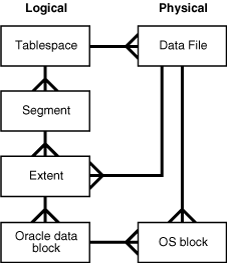
\includegraphics[width=0.4\textwidth]{Pictures/Task_1/oracle-logical-storage.png}
    \caption{Cấu trúc lưu trữ logic và vật lý (Nguồn: Oracle Database Concepts \cite{oracleLogicalStorage}).}
    \label{fig:st-oracle-logical-physical-storage}
\end{figure}

Mô hình lưu trữ đĩa cứng kết hợp với Redo Log, Database Buffer Cache và cơ chế kiểm soát giao dịch ACID giúp Oracle duy trì tính toàn vẹn dữ liệu nghiêm ngặt, hỗ trợ khôi phục sau sự cố và đảm bảo khả năng mở rộng cho hệ thống \cite{oracleLogicalStorage}.

\paragraph{Redis}

Khác với Oracle, Redis là một cơ sở dữ liệu NoSQL dạng key-value hoạt động hoàn toàn trên bộ nhớ trong \cite{redisDataTypes}.
\begin{itemize}[label=--]
    \item \textbf{In-memory Keyspace và bộ cấp phát bộ nhớ:} Toàn bộ dữ liệu được tổ chức dưới dạng keyspace và duy trì trực tiếp trong RAM. Redis sử dụng bộ cấp phát \texttt{jemalloc} để quản lý các khối RAM và tối ưu hóa memory overhead. Để bảo vệ bộ nhớ, hệ thống hỗ trợ các eviction policy như \texttt{allkeys-lru} khi vượt quá ngưỡng \texttt{maxmemory}.
    
    \item \textbf{Cấu trúc RedisJSON:} Phân hệ mở rộng RedisJSON nâng cấp Redis thành một document store. Dữ liệu JSON được phân tích cú pháp và lưu trữ dưới dạng cấu trúc cây binary trong RAM, cho phép truy xuất và sửa đổi các nested field với độ phức tạp $O(1)$ hoặc $O(N)$ mà không cần encode hoặc decode lại toàn bộ chuỗi văn bản \cite{redisJson}.
    
    \item \textbf{Cơ chế Persistence:} Mặc dù hoạt động trên RAM, Redis hỗ trợ hai cơ chế ghi đĩa bền vững bao gồm tạo snapshot RDB (Redis Database Backup) và ghi nhật ký AOF (Append-Only File) \cite{redisPersistence}.
\end{itemize}

Tuy nhiên, cấu trúc lưu trữ của Redis không tự động quản lý các mối quan hệ liên kết như foreign key giữa các document, cũng như không tự động áp dụng các ràng buộc schema ở cấp độ cơ sở dữ liệu.

\paragraph{So sánh tổng quan kiến trúc}

Sự khác biệt về kiến trúc lưu trữ tạo ra tính chất kỹ thuật đối lập giữa hai hệ thống: Oracle tập trung vào tính toàn vẹn, tính bền vững và đóng vai trò là source of truth nghiêm ngặt; trong khi Redis tối ưu triệt để cho hiệu năng đọc ghi tốc độ cao với độ trễ sub-millisecond. Sự kết hợp cả hai hệ thống trong ShopFlash chính là bài toán khai thác ưu điểm kiến trúc của từng phía.

\subsubsection{Thiết kế lưu trữ trong kiến trúc ShopFlash}

Oracle đóng vai trò là source of truth. Ba bảng \texttt{CATEGORIES}, \texttt{PRODUCTS} và \texttt{PRODUCT\_INVENTORY} chứa dữ liệu catalog, quan hệ Category--Product và tồn kho. Product có foreign key tới Category; SKU và slug có unique constraint; giá và số lượng tồn kho được bảo vệ thêm bằng check constraint \cite{oracleConstraints}. Bảng ProductInventory tách khỏi Product để luồng Storage chỉ cập nhật \texttt{on\_hand\_quantity}, còn số lượng đã giữ cho Flash Sale thuộc module concurrency.

Redis không lưu một bản sao đầy đủ của mô hình quan hệ. Với mỗi Product, backend tạo một RedisJSON document có key \texttt{product:\{id\}} gồm các trường \texttt{id}, \texttt{sku}, \texttt{name}, \texttt{categoryId}, \texttt{categoryName}, \texttt{price}, \texttt{status}, \texttt{inStock} và \texttt{thumbnailUrl}. Category, Inventory, foreign key và unique SKU không được Redis sở hữu. Mọi thao tác CRUD đi qua Oracle bằng JDBC; chỉ sau khi transaction Oracle commit thành công, backend mới cập nhật product projection Redis. Khi Redis lỗi, Oracle không rollback; projection có thể được dựng lại từ Oracle.

\begin{table}[H]
    \centering
    \caption{Trách nhiệm dữ liệu của Oracle và Redis trong ShopFlash}
    \label{tab:st-storage-model-mapping}
    \begin{tabularx}{\textwidth}{@{}p{0.24\textwidth}XX@{}}
        \toprule
        Thành phần & Oracle & Redis \\
        \midrule
        Category & Dòng trong \texttt{CATEGORIES}; là dữ liệu gốc. & Không có Category document độc lập. \\
        Product & Dòng trong \texttt{PRODUCTS}; là dữ liệu gốc. & Document phái sinh \texttt{product:\{id\}}. \\
        Inventory & \texttt{PRODUCT\_INVENTORY}, có version để optimistic locking. & Chỉ suy ra \texttt{inStock} trong product projection. \\
        Quan hệ và ràng buộc & Foreign key Product--Category, unique SKU/slug, check constraint giá và tồn kho. & Không có foreign key, unique hay check constraint khai báo. \\
        Đồng bộ & Commit transaction trước. & Cập nhật sau commit; có API rebuild khi projection stale. \\
        \bottomrule
    \end{tabularx}
\end{table}

\subsubsection{Đánh giá thực nghiệm}

\paragraph{Toàn vẹn dữ liệu (E1)}

\noindent\textbf{Phương pháp}\par

Màn hình so sánh Oracle–Redis liệt kê các ràng buộc được bảo vệ ở form API và Oracle. Để chứng minh RedisJSON không có constraint khai báo tương đương, backend tạo một document kiểm thử có \texttt{categoryId = 999999999} (không tham chiếu Category Oracle nào) và \texttt{price = -1} (vi phạm điều kiện \texttt{base\_price >= 0} của Oracle). Document này được ghi trực tiếp vào key ngẫu nhiên \texttt{storage-lab:constraint-demo:\{uuid\}}, đọc lại bằng \texttt{JSON.GET}, rồi xóa bằng \texttt{UNLINK} ngay trong cùng request. Key kiểm thử không có prefix \texttt{product:}, nên không đi vào product projection hoặc Redis search index. Thử nghiệm không ghi Oracle và không làm thay đổi dữ liệu Category hoặc Product thật.

\noindent\textbf{Kết quả và phân tích}\par
Hình~\ref{fig:st-storage-lab-integrity} cho thấy RedisJSON nhận document không hợp lệ. Đây không phải lỗi của Redis; RedisJSON là document store linh hoạt và không tự kiểm tra foreign key hay check condition của schema Oracle. Trong kiến trúc ShopFlash, client không được ghi trực tiếp vào Redis: request hợp lệ phải qua API, Oracle là lớp thực thi ràng buộc cuối cùng, còn Redis chỉ nhận projection đã được backend tạo.

\begin{figure}[H]
    \centering
    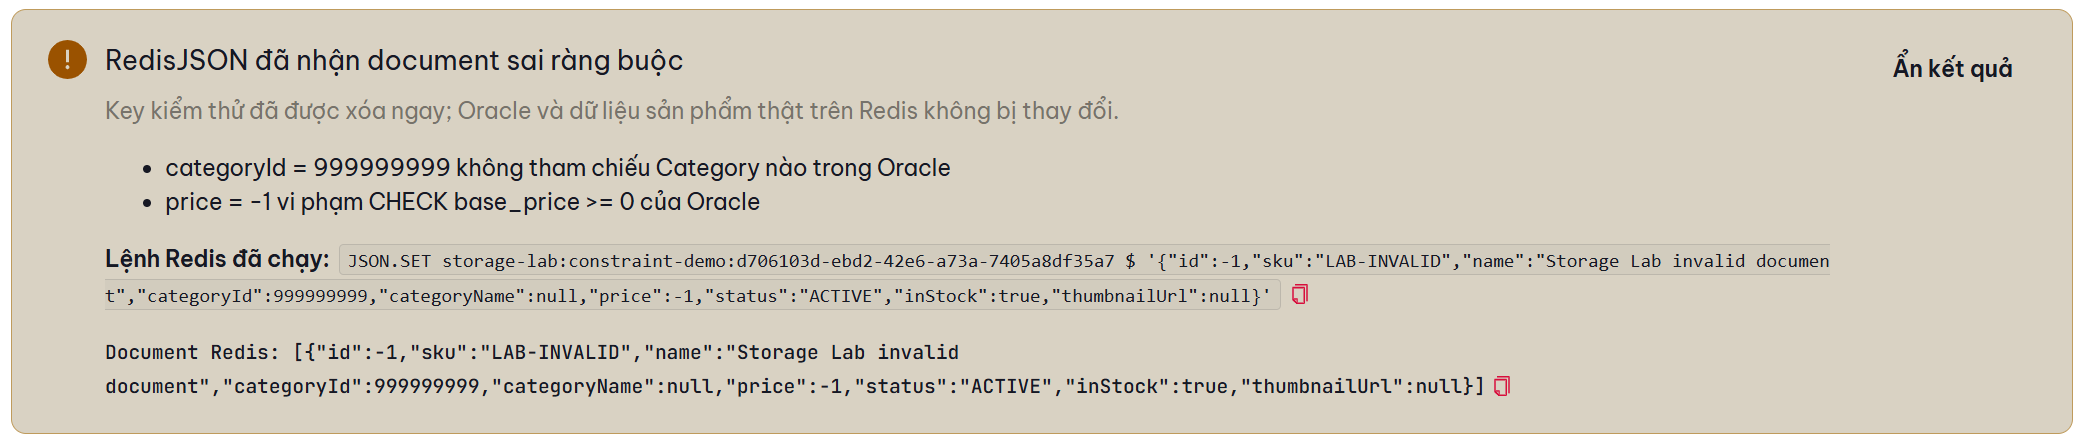
\includegraphics[width=0.8\textwidth]{Pictures/Task_1/storage-lab-constraint-demo.png}
    \caption{E1: RedisJSON nhận document có Category không tồn tại và giá âm; key kiểm thử được dọn ngay sau khi đọc.}
    \label{fig:st-storage-lab-integrity}
\end{figure}

\begin{table}[H]
    \centering
    \caption{Kết luận E1 trong kiến trúc ShopFlash}
    \label{tab:st-integrity-results}
    \begin{tabularx}{\textwidth}{@{}p{0.3\textwidth}XX@{}}
        \toprule
        Quy tắc & Oracle (source of truth) & Redis projection \\
        \midrule
        Category phải tồn tại & Foreign key \texttt{PRODUCTS.category\_id} chặn dữ liệu mồ côi. & Document ghi trực tiếp vẫn có thể chứa \texttt{categoryId} không tồn tại. \\
        SKU không trùng & Unique constraint và kiểm tra của API. & Không dùng làm nơi kiểm tra unique SKU. \\
        Giá không âm & \texttt{CHECK (base\_price >= 0)} và validation API. & Document ghi trực tiếp vẫn có thể chứa \texttt{price = -1}. \\
        Tồn kho không thấp hơn phần đã giữ & Check constraint trên ProductInventory, API kiểm tra và optimistic locking. & Chỉ nhận trường \texttt{inStock} đã suy ra; không quản lý số lượng gốc. \\
        \bottomrule
    \end{tabularx}
\end{table}

\paragraph{Dung lượng lưu trữ (Footprint) (E2)}

\noindent\textbf{Phương pháp}\par
Endpoint \texttt{GET /api/admin/catalog/storage-footprint} đọc \texttt{USER\_}\allowbreak\texttt{SEGMENTS} cho ba table segment và các index segment liên quan trực tiếp đến \texttt{CATEGORIES}, \texttt{PRODUCTS}, \texttt{PRODUCT\_INVENTORY}. Các bảng khác trong cơ sở dữ liệu hệ thống ShopFlash không nằm trong phạm vi tính toán của thử nghiệm này. Tổng dung lượng của Oracle vì thế là dung lượng đã cấp phát (allocated bytes) dành riêng cho phân hệ danh mục catalog, không phải số byte dữ liệu thực tế đang sử dụng của toàn bộ cơ sở dữ liệu. Oracle cấp phát không gian theo extent và thường giữ lại dung lượng đã cấp để tái sử dụng sau khi xóa dòng \cite{oracleLogicalStorage}.

Ở phía Redis, endpoint quét đúng các key \texttt{product:*} và cộng kết quả từ lệnh \texttt{MEMORY USAGE} của từng key \cite{redisMemoryUsage}. Lệnh này trả về lượng bộ nhớ tính bằng byte của một key cùng giá trị đi kèm. Số liệu của Redis không bao gồm bộ nhớ nền của Redis server, Docker container hay bộ nhớ của RediSearch index. Vì vậy, thử nghiệm E2 thực chất so sánh footprint vận hành của dữ liệu gốc trên Oracle với product projection trên Redis, không phải so sánh hai mô hình dữ liệu tương đương hoàn toàn.

\noindent\textbf{Kết quả và phân tích}\par
Sau khi gọi rebuild projection, Oracle có 1\,000 Product và Redis có 1\,000 document; trạng thái projection hoàn toàn đồng bộ. Bảng~\ref{tab:st-storage-footprint-results} ghi lại snapshot thu được từ Storage Lab.

\begin{table}[H]
    \centering
    \caption{Snapshot footprint với 100 Category và 1\,000 Product}
    \label{tab:st-storage-footprint-results}
    \begin{tabularx}{\textwidth}{@{}X r r@{}}
        \toprule
        Hệ / Phạm vi đo & \multicolumn{1}{c}{Dung lượng (bytes)} & \multicolumn{1}{c}{Bytes trên một Product/document} \\
        \midrule
        Oracle: 3 table và index catalog đã cấp phát & 1\,245\,184 & 1\,245.18 \\
        Redis: Các RedisJSON key \texttt{product:*} & 575\,000 & 575.00 \\
        \bottomrule
    \end{tabularx}
\end{table}

Chi tiết segment Oracle trong Hình~\ref{fig:st-storage-lab-segments} cho thấy ba table segment chiếm 458\,752 bytes; các index segment (bao gồm cả LOB index của cột mô tả Product) chiếm 786\,432 bytes. Dung lượng allocated của Oracle lớn hơn Redis projection 670\,184 bytes trong snapshot này. Kết quả này phản ánh đúng vai trò khác nhau giữa hai hệ thống: Oracle lưu dữ liệu gốc, thông tin tồn kho cùng nhiều chỉ mục để đảm bảo tính toàn vẹn và hỗ trợ truy vấn; trong khi Redis chỉ lưu trữ document projection để phục vụ đọc nhanh.

\begin{figure}[H]
    \centering
    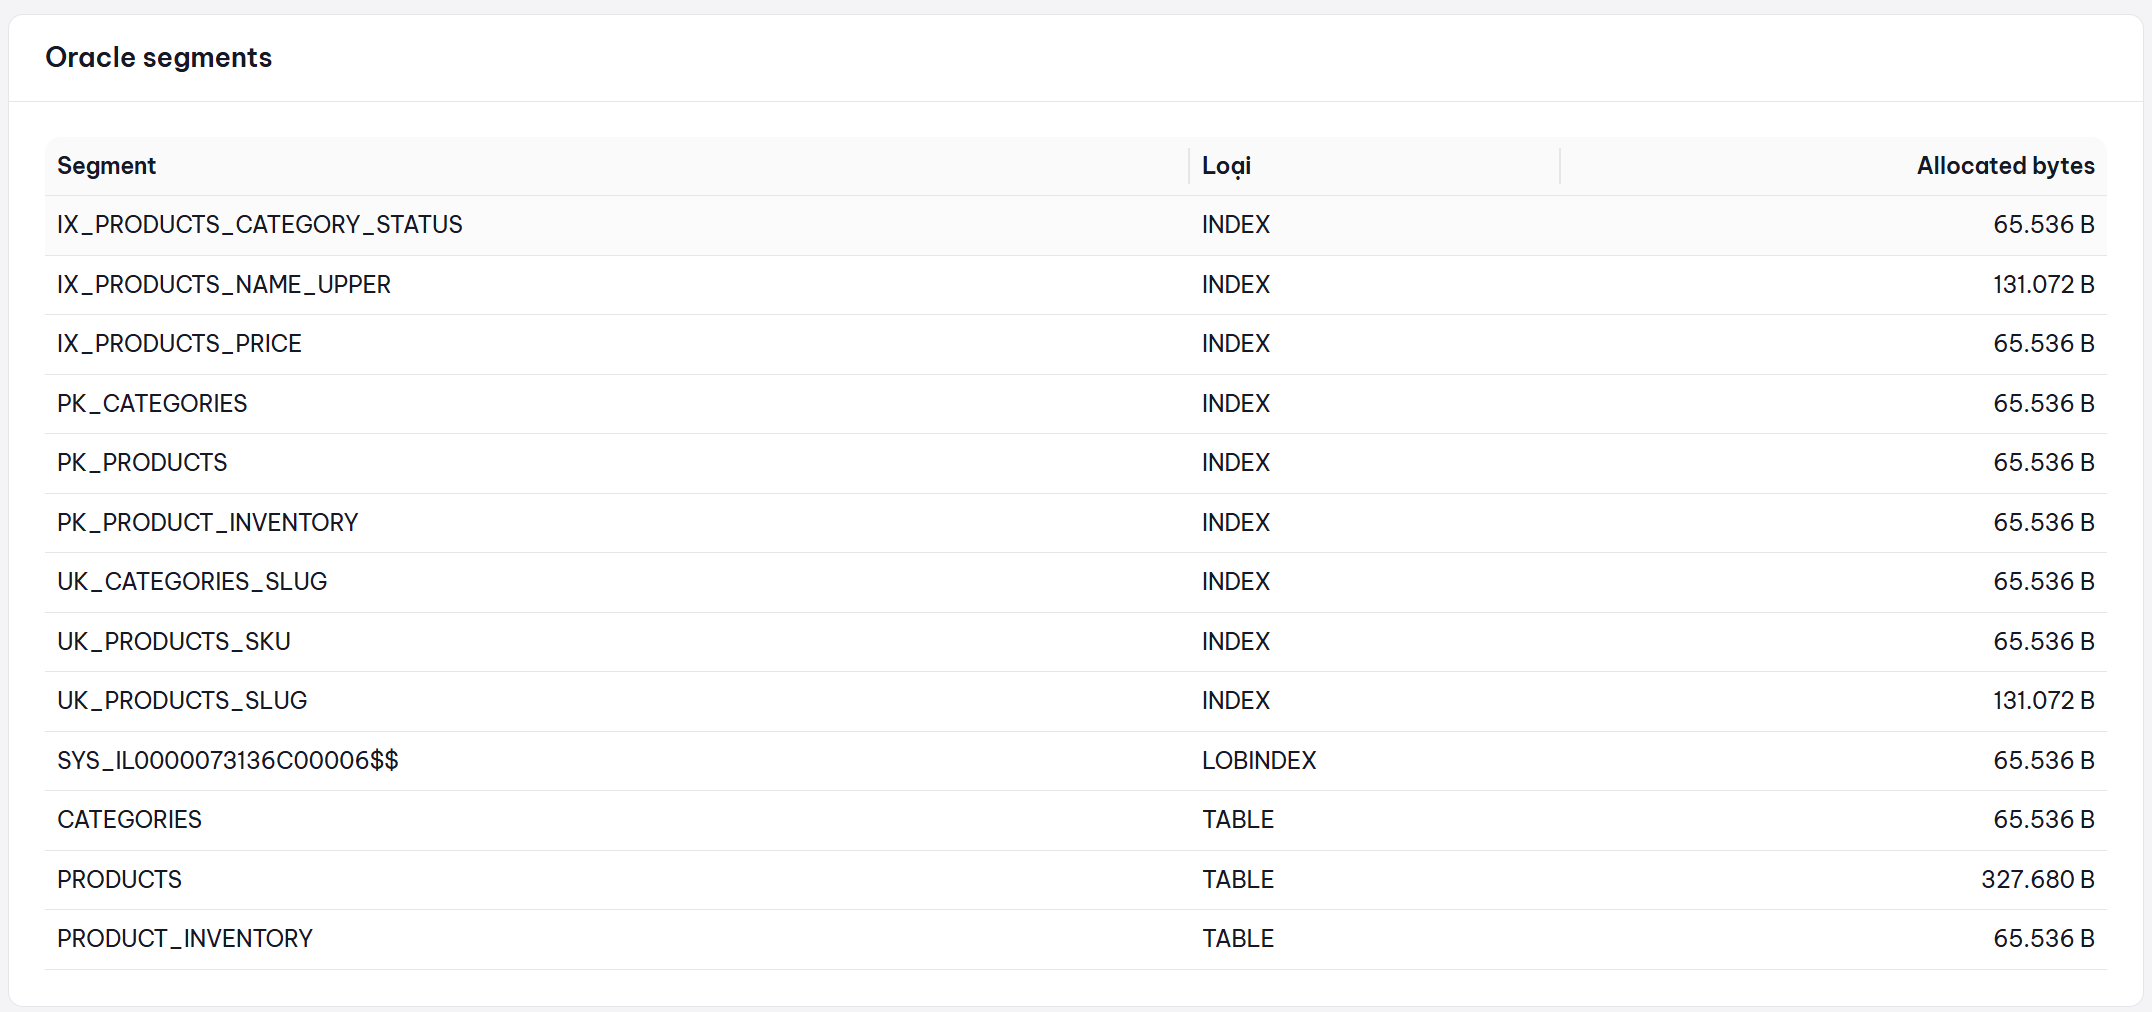
\includegraphics[width=\textwidth]{Pictures/Task_1/storage-lab-segments.png}
    \caption{Các Oracle table và index segment được cộng vào footprint E2.}
    \label{fig:st-storage-lab-segments}
\end{figure}

Số liệu thực nghiệm này không dùng để suy rộng rằng Redis luôn tốn ít dung lượng hơn Oracle trong mọi trường hợp. Kết quả thực tế phụ thuộc vào bản chất dữ liệu, cấu trúc schema, số lượng chỉ mục, cơ chế cấp phát block hoặc extent của Oracle và cách thiết kế cấu trúc JSON trong Redis.

\subsubsection{Đánh giá tổng hợp và định hướng sử dụng DBMS}

Kết quả thực nghiệm E1 và E2 thể hiện rõ sự đánh đổi kỹ thuật giữa hai hệ quản trị cơ sở dữ liệu trong hệ thống ShopFlash:

\begin{itemize}[label=--]
    \item \textbf{Oracle Database} thể hiện ưu thế tuyệt đối ở vai trò source of truth nhờ cơ chế quản lý giao dịch ACID nghiêm ngặt và khả năng cưỡng chế các ràng buộc toàn vẹn ngay tại cấp độ cơ sở dữ liệu. Mặc dù chi phí footprint lưu trữ ban đầu cao hơn do phải duy trì các cấu trúc phân cấp (block, extent, segment) cùng chỉ mục phục vụ ràng buộc, đây là chi phí bắt buộc để bảo vệ tính chính xác của dữ liệu nghiệp vụ gốc.
    \item \textbf{Redis} đạt hiệu quả cao ở luồng đọc nhờ cấu trúc dữ liệu tối ưu trực tiếp trên bộ nhớ trong, giúp giảm footprint trên từng document phái sinh. Tuy nhiên, việc thiếu các cơ chế kiểm soát schema hay quan hệ liên kết tự động khiến Redis không thích hợp làm nơi thực thi quy tắc nghiệp vụ gốc.
\end{itemize}

Từ những phân tích trên, kiến trúc kết hợp Hybrid cho phân hệ danh mục ShopFlash là lựa chọn tối ưu. Oracle được sử dụng làm nơi thực thi chính cho toàn bộ thao tác ghi, quản lý dữ liệu Category, Product và Inventory. Redis đóng vai trò là một lớp cản đọc (read buffer), tiếp nhận các product projection phái sinh từ Oracle để phục vụ người dùng cuối với tốc độ cao. Mô hình này giúp hệ thống vừa đạt hiệu năng đọc tối ưu của cơ sở dữ liệu in-memory, vừa giữ vững tính toàn vẹn dữ liệu nghiêm ngặt của cơ sở dữ liệu quan hệ truyền thống.
\endgroup

% !TeX root = ../../main.tex
\subsection{Indexing}\label{sec:indexing}
\begingroup
% Đánh số bảng/hình/mã nguồn theo mục (2.2.x), giống Storage và Transaction.
\setcounter{table}{0}\setcounter{figure}{0}\setcounter{lstlisting}{0}
\renewcommand{\thetable}{\thesubsection.\arabic{table}}
\renewcommand{\thefigure}{\thesubsection.\arabic{figure}}
\renewcommand{\thelstlisting}{\thesubsection.\arabic{lstlisting}}
\renewcommand{\theHtable}{\thesubsection.\arabic{table}}
\renewcommand{\theHfigure}{\thesubsection.\arabic{figure}}
\def\theHlstlisting{\thesubsection.\arabic{lstlisting}}

\subsubsection{Mục tiêu, phạm vi và câu hỏi nghiên cứu}\label{sec:ix-goal}

Tìm kiếm và duyệt sản phẩm là một trong những luồng đọc dữ liệu diễn ra thường xuyên nhất của khách hàng trong ShopFlash. Khách hàng tìm theo từ khóa, chọn danh mục, lọc theo khoảng giá rồi sắp xếp và lật từng trang kết quả; trong khi đó, việc thêm hoặc sửa thông tin sản phẩm do quản trị viên thực hiện thưa hơn nhiều. Đây là một khối lượng công việc \emph{đọc nhiều, ghi ít}. Với khối lượng công việc này, chỉ mục (\emph{index}) là công cụ chính để rút ngắn thời gian truy vấn. Tuy nhiên, chỉ mục không miễn phí: mỗi chỉ mục chiếm thêm dung lượng, làm chậm các thao tác ghi, và phải luôn phản ánh đúng dữ liệu gốc.

Mục này nghiên cứu cách Oracle Database và Redis giải quyết bài toán chỉ mục, và đối chiếu chúng trên chính các truy vấn của ShopFlash. Như đã trình bày ở mục~\ref{sec:storage}, Oracle là nguồn dữ liệu gốc của danh mục và sản phẩm, còn Redis giữ một bản chiếu (\emph{projection}) của từng sản phẩm dưới dạng tài liệu RedisJSON \texttt{product:\{id\}}, được đánh chỉ mục bằng RediSearch trong chỉ mục \texttt{idx:products}. Vì vậy, mỗi yêu cầu tìm kiếm của khách hàng có thể được phục vụ bởi Oracle hoặc bởi Redis, và câu hỏi cần trả lời là nên giao yêu cầu nào cho DBMS nào.

Bảng~\ref{tab:ix-query-patterns} tóm tắt các nội dung được dùng làm đối tượng nghiên cứu, ứng với sáu thí nghiệm E1 đến E6. Ba thí nghiệm đầu là các mẫu truy vấn đọc, được chọn để trải từ truy vấn cực kỳ chọn lọc (chỉ một dòng kết quả) đến truy vấn trả về hàng nghìn dòng, vì hiệu quả của chỉ mục phụ thuộc mạnh vào số dòng được chọn ra; thí nghiệm thứ tư là thao tác ghi. Hai thí nghiệm còn lại không gắn với một câu truy vấn cụ thể mà xét cái giá của chỉ mục: dung lượng mà chỉ mục chiếm (E5) và thời điểm chỉ mục phản ánh một thay đổi dữ liệu (E6).

\begin{table}[!htbp]
\centering
\caption{Các mẫu truy vấn và khía cạnh của chỉ mục được nghiên cứu.}\label{tab:ix-query-patterns}
\reporttablesetup
\begin{tabularx}{\linewidth}{|>{\hsize=1.1\hsize\linewidth=\hsize}L|>{\hsize=0.8\hsize\linewidth=\hsize}L|>{\hsize=1.1\hsize\linewidth=\hsize}L|c|}
\hline
\rowcolor{ReportTableHead}
\reportheader{Nội dung nghiên cứu} & \reportheader{Chức năng} & \reportheader{Ví dụ} & \reportheader{Thí nghiệm} \\ \hline
Tra cứu theo một khóa duy nhất, cùng cơ chế với ràng buộc SKU duy nhất của sản phẩm & Nền tảng của mọi kiểu tra cứu & Tìm sản phẩm có SKU \texttt{LAB-0123456} & E1 \\ \hline
Tìm từ khóa trong tên sản phẩm & Tìm kiếm sản phẩm & ``sony pro'': hai từ khóa, mỗi từ khớp nguyên từ & E2 \\ \hline
Lọc theo danh mục và khoảng giá, sắp xếp theo giá, phân trang & Lọc nâng cao & Danh mục số 5, giá từ 1 đến 5 triệu đồng, giá tăng dần, 24 sản phẩm mỗi trang & E3 \\ \hline
Ghi dữ liệu: thêm sản phẩm, sửa giá & Quản lý sản phẩm của quản trị viên & Thêm sản phẩm mới; đổi giá một sản phẩm & E4 \\ \hline
Dung lượng mà chỉ mục chiếm thêm & Mọi chức năng tìm kiếm có dùng chỉ mục & Dung lượng chỉ mục của E1 đến E3: trên đĩa (Oracle) và trong RAM (Redis) & E5 \\ \hline
Thời điểm chỉ mục phản ánh thay đổi dữ liệu & Kết quả tìm kiếm đúng sau khi sản phẩm thay đổi & Thêm, sửa giá, xóa một sản phẩm rồi tìm lại ngay & E6 \\ \hline
\end{tabularx}
\end{table}

Từ bối cảnh trên, mục này tìm câu trả lời cho ba câu hỏi nghiên cứu:

\begin{enumerate}[label=(\arabic*),leftmargin=*,itemsep=2pt,topsep=4pt]
    \item Với từng mẫu truy vấn đọc trong Bảng~\ref{tab:ix-query-patterns} (E1 đến E3), chỉ mục trên Oracle và trên Redis giúp truy vấn nhanh hơn bao nhiêu so với khi không có chỉ mục?
    \item Cái giá của chỉ mục là gì: thao tác ghi chậm đi bao nhiêu, chiếm thêm bao nhiêu dung lượng, và chỉ mục phản ánh thay đổi dữ liệu vào thời điểm nào?
    \item Từ đó, việc tìm kiếm và lọc sản phẩm của ShopFlash nên giao cho DBMS nào, với loại chỉ mục nào, cho từng loại yêu cầu?
\end{enumerate}

\paragraph*{Phạm vi}

Nghiên cứu giới hạn ở phân hệ danh mục và sản phẩm của ShopFlash, trên hai hệ quản trị Oracle Database và Redis (kèm mô-đun RediSearch). Để chênh lệch giữa các cách truy cập đủ lớn để đo được, các thí nghiệm không chạy trên dữ liệu thật của ứng dụng mà trên một tập 200\,000 sản phẩm giả, được sinh theo cùng một công thức ở cả hai hệ quản trị và đặt trong đối tượng riêng (một bảng riêng trên Oracle và các khóa có tiền tố riêng trên Redis), không làm thay đổi dữ liệu của ứng dụng. Kết quả đo được dùng để quyết định cách hiện thực tìm kiếm và lọc trong ShopFlash.

Mục này không xét các truy vấn kết nối nhiều bảng và các báo cáo thống kê; những nội dung đó thuộc về mục~\ref{sec:query} (Query Processing).

\subsubsection{Cơ sở lý thuyết về chỉ mục}\label{sec:ix-theory}

Mục này xây dựng khung lý thuyết để trả lời ba câu hỏi nghiên cứu. Trước hết, chỉ mục được định nghĩa và gắn với ba chiều đánh giá tương ứng với các câu hỏi đó, trên cả hai hệ quản trị. Tiếp theo, các cấu trúc chỉ mục của Oracle và Redis được phân loại theo kiểu truy vấn mà chúng phục vụ. Cuối cùng, mục này so sánh cách hai hệ quản trị lựa chọn cách truy cập và duy trì chỉ mục khi dữ liệu thay đổi.

\paragraph{Chỉ mục và ba chiều đánh giá}\label{sec:ix-dimensions}

Chỉ mục (\emph{index}) là một cấu trúc dữ liệu phụ, được tạo thêm bên cạnh dữ liệu gốc để tìm nhanh các bản ghi thỏa một điều kiện mà không phải duyệt toàn bộ dữ liệu. 

Khi không có chỉ mục, hai hệ quản trị phải duyệt toàn bộ dữ liệu theo hai cách khác nhau. Oracle lưu dữ liệu bảng thành các khối (\emph{block}), thường 8~KB mỗi khối như đã nêu ở mục~\ref{sec:storage}; nếu không có chỉ mục phù hợp, truy vấn phải đọc lần lượt mọi khối của bảng, gọi là quét toàn bảng (\emph{full table scan}), và số khối phải đọc tăng tỉ lệ thuận với kích thước bảng. Redis lưu dữ liệu dưới dạng các cặp key--value trong bộ nhớ và về mặt gốc chỉ tra cứu theo tên key \cite{redisSecondaryIndexing}. Muốn tìm theo giá trị nằm bên trong một tài liệu, chẳng hạn các sản phẩm có giá trong một khoảng, mà không có chỉ mục, thì phải duyệt lần lượt mọi key bằng lệnh \texttt{SCAN} rồi đọc từng tài liệu để kiểm tra điều kiện; đây cũng là cách ``không có chỉ mục'' được dùng làm mốc so sánh trong các thí nghiệm. Với cả hai hệ quản trị, chỉ mục thay việc duyệt toàn bộ bằng việc đi thẳng tới các bản ghi cần tìm.

Lợi ích của chỉ mục phụ thuộc vào độ chọn lọc (\emph{selectivity}) của điều kiện lọc: điều kiện càng chọn ra ít dòng thì độ chọn lọc càng cao. Theo tài liệu của Oracle, đường truy cập qua chỉ mục hiệu quả hơn khi truy vấn lấy một phần nhỏ của bảng, còn khi truy vấn cần phần lớn các khối của bảng thì quét toàn bảng hiệu quả hơn; khi đó bộ tối ưu chọn quét toàn bảng dù có chỉ mục \cite{oracleAccessPaths}. Ảnh hưởng của độ chọn lọc lên cả hai hệ quản trị được khảo sát ở thí nghiệm E2, nơi cùng một kiểu truy vấn được thử với ba từ khóa khớp số dòng rất khác nhau.

Mặt khác, chỉ mục không miễn phí. Vì vậy nghiên cứu đánh giá một chỉ mục trên ba chiều:

\begin{itemize}[label=--,leftmargin=*,itemsep=2pt,topsep=4pt]
    \item \textbf{Tốc độ truy vấn đọc:} chỉ mục giúp truy vấn nhanh hơn bao nhiêu so với duyệt toàn bộ dữ liệu.
    \item \textbf{Chi phí duy trì:} dung lượng chỉ mục chiếm thêm, và mức làm chậm các thao tác ghi, vì mỗi lần dữ liệu được thêm, sửa hoặc xóa, hệ quản trị hoặc ứng dụng phải cập nhật cả chỉ mục. Ở Oracle, nhiều chỉ mục trên một bảng làm các thao tác ghi chậm đi vì hệ quản trị phải cập nhật tất cả các chỉ mục đó \cite{oracleIndexes}. Ở Redis, chỉ mục do RediSearch lập được cập nhật cùng với lệnh ghi \cite{redisJsonIndexing}, còn chỉ mục tự dựng thì do ứng dụng cập nhật \cite{redisSecondaryIndexing}.
    \item \textbf{Tính nhất quán:} thời điểm chỉ mục phản ánh một thay đổi dữ liệu, tức sau bao lâu thì kết quả tìm kiếm qua chỉ mục thấy được thay đổi đó.
\end{itemize}

Chiều thứ nhất ứng với câu hỏi nghiên cứu (1), hai chiều còn lại ứng với câu hỏi (2). Dung lượng của hai hệ quản trị có bản chất khác nhau: chỉ mục của Oracle nằm trên đĩa, còn chỉ mục của Redis nằm trong bộ nhớ (mục~\ref{sec:storage}), nên hai con số này không thể so sánh trực tiếp với nhau.

\paragraph{Cấu trúc chỉ mục theo kiểu truy vấn}\label{sec:ix-structures}

Mỗi kiểu truy vấn trong Bảng~\ref{tab:ix-query-patterns} cần một cấu trúc chỉ mục khác nhau. Phần này lần lượt giải thích cấu trúc phù hợp với từng kiểu, và Bảng~\ref{tab:ix-index-types} ở cuối phần tóm tắt lại.

\noindent\textbf{Tìm bằng, tìm theo khoảng và sắp xếp.} Oracle dùng chỉ mục B-tree cho các kiểu truy vấn này. Chỉ mục được tổ chức thành một cây nhiều tầng (Hình~\ref{fig:ix-btree}): các khối nhánh (\emph{branch block}) chứa các mốc để điều hướng, còn các khối lá (\emph{leaf block}) chứa giá trị khóa kèm định danh dòng (\emph{ROWID}), tức địa chỉ cho biết dòng dữ liệu nằm ở đâu \cite{oracleIndexes}. Để tìm một khóa, hệ quản trị đi từ gốc xuống lá qua vài tầng. Cây luôn cân bằng, nghĩa là mọi khối lá nằm cùng độ sâu, nên tìm bất kỳ bản ghi nào cũng mất gần như cùng thời gian. Các khối lá còn được nối với nhau theo hai chiều, nên sau khi tìm thấy khóa đầu của một khoảng, hệ quản trị chỉ việc đi ngang qua các lá liên tiếp để lấy cả khoảng; và vì khóa đã được sắp xếp sẵn, kết quả cũng được trả theo thứ tự mà không cần sắp xếp lại \cite{oracleIndexes}.

\begin{figure}[!htbp]
\centering
\begin{tikzpicture}[
  nodebox/.style={draw,rectangle,minimum height=7mm,inner xsep=6pt,font=\small},
  branch/.style={nodebox,fill=ReportTableHead},
  leaf/.style={nodebox,fill=white},
  >=Stealth]
  \node[branch] (root) at (0,0) {30 \hspace{1em} 60};
  \node[leaf] (a) at (-4.2,-2) {10 \hspace{1em} 20};
  \node[leaf] (b) at (0,-2) {30 \hspace{1em} 40 \hspace{1em} 50};
  \node[leaf] (c) at (4.2,-2) {60 \hspace{1em} 70 \hspace{1em} 80};
  \draw[->] (root.south) -- (a.north);
  \draw[->] (root.south) -- (b.north);
  \draw[->] (root.south) -- (c.north);
  \draw[<->] (a.east) -- (b.west);
  \draw[<->] (b.east) -- (c.west);
  \node[anchor=west,font=\small] at (1.4,0) {khối nhánh (điều hướng)};
  \node[anchor=north,font=\small] at (0,-2.5) {khối lá (khóa và ROWID), nối với nhau};
\end{tikzpicture}
\caption{Cấu trúc B-tree minh họa: khối nhánh dẫn xuống các khối lá, các khối lá nối với nhau để đọc một khoảng giá trị.}\label{fig:ix-btree}
\end{figure}

Redis, như đã nói, chỉ tra cứu theo tên key, nên chỉ mục phụ phải được dựng thêm. Có hai hướng. Hướng thứ nhất là ứng dụng tự dựng chỉ mục bằng các cấu trúc dữ liệu của Redis \cite{redisSecondaryIndexing}: một key riêng ánh xạ giá trị cần tìm tới mã đối tượng (ví dụ từ SKU tới mã sản phẩm) phục vụ tìm bằng; và Sorted Set, một tập hợp trong đó mỗi phần tử có một điểm số và các phần tử luôn được giữ theo thứ tự điểm. Nếu chọn phần tử là mã sản phẩm và điểm là giá, thì một lệnh \texttt{ZRANGE} kèm \texttt{BYSCORE} trả về các sản phẩm có giá trong một khoảng, đã xếp sẵn theo giá \cite{redisSecondaryIndexing}. Hướng thứ hai là dùng mô-đun RediSearch, trong đó chỉ mục được khai báo bằng lệnh \texttt{FT.CREATE} trên các trường của tài liệu JSON: trường kiểu \texttt{TAG} phục vụ khớp chính xác một giá trị, trường kiểu \texttt{NUMERIC} phục vụ tìm theo khoảng số, và tùy chọn \texttt{SORTABLE} cho phép sắp xếp theo trường với độ trễ rất thấp nhưng tốn thêm bộ nhớ \cite{redisFtCreate}.

\noindent\textbf{Nhiều điều kiện cùng lúc.} Truy vấn thực tế thường có nhiều điều kiện, chẳng hạn ``danh mục số 5 và giá từ 100 đến 500 nghìn đồng''. Oracle dùng chỉ mục nhiều cột (\emph{composite index}): các mục được sắp xếp theo cột thứ nhất, trong cùng một giá trị của cột thứ nhất lại sắp theo cột thứ hai, và cứ thế. Bảng~\ref{tab:ix-composite-example} minh họa trên sáu sản phẩm. Với chỉ mục (danh mục, giá), các sản phẩm cùng một danh mục nằm liền nhau và đã xếp theo giá, nên truy vấn trên chỉ phải đọc đúng đoạn liên tiếp thỏa cả hai điều kiện. Với chỉ mục (giá, danh mục), đoạn thỏa điều kiện giá có cả sản phẩm của danh mục khác (ở ví dụ là mục (300, 2)), nên hệ quản trị phải đọc rồi loại bớt. Vì vậy thứ tự cột là yếu tố quyết định: chỉ mục chỉ được dùng hiệu quả khi truy vấn có điều kiện trên cột đầu hoặc phần đầu của dãy cột. Chẳng hạn, một chỉ mục trên (\texttt{last\_name}, \texttt{job\_id}, \texttt{salary}) không được dùng cho truy vấn không nhắc tới \texttt{last\_name} \cite{oracleIndexes}. Quy tắc thiết kế được kiểm chứng ở thí nghiệm E3 là đặt các cột so sánh bằng trước, các cột khoảng và cột sắp xếp sau.

\begin{table}[!htbp]
\centering
\caption{Ví dụ thứ tự các mục trong hai chỉ mục nhiều cột (giá tính bằng nghìn đồng). Chữ đậm là các mục thỏa ``danh mục 5, giá từ 100 đến 500''.}\label{tab:ix-composite-example}
\reporttablesetup
\begin{tabularx}{\linewidth}{|>{\hsize=0.7\hsize\linewidth=\hsize}L|>{\hsize=1.3\hsize\linewidth=\hsize}L|}
\hline
\rowcolor{ReportTableHead}
\reportheader{Cấu trúc} & \reportheader{Các mục theo thứ tự lưu} \\ \hline
Dữ liệu (danh mục, giá), theo thứ tự thêm vào & (2, 90), (5, 150), (5, 280), (2, 300), (2, 700), (5, 900) \\ \hline
Chỉ mục (danh mục, giá) & (2, 90), (2, 300), (2, 700), \textbf{(5, 150)}, \textbf{(5, 280)}, (5, 900) \\ \hline
Chỉ mục (giá, danh mục) & (90, 2), \textbf{(150, 5)}, \textbf{(280, 5)}, (300, 2), (700, 2), (900, 5) \\ \hline
\end{tabularx}
\end{table}

Với Redis, RediSearch kết hợp các điều kiện đặt trên từng trường đã khai báo. Còn với chỉ mục tự dựng, một cách là tạo một Sorted Set riêng cho mỗi giá trị của cột so sánh bằng, ví dụ mỗi danh mục một Sorted Set với điểm là giá; truy vấn trên khi đó chỉ cần lấy khoảng giá trong Sorted Set của danh mục số 5. Cách khác là dùng Sorted Set theo thứ tự từ điển, ghép nhiều cột thành một chuỗi khóa \cite{redisSecondaryIndexing}.

\noindent\textbf{Từ nằm trong chuỗi.} Tìm một từ trong tên sản phẩm, chẳng hạn ``sony'', là kiểu truy vấn mà B-tree phục vụ kém. B-tree sắp xếp các chuỗi theo thứ tự từ ký tự đầu, nên chỉ hữu ích khi biết phần đầu của chuỗi, ví dụ các tên bắt đầu bằng ``Tai nghe''. Từ cần tìm lại thường nằm giữa tên, như trong ``Tai nghe Sony Pro'', và điều kiện \texttt{LIKE '\%sony\%'} có ký tự đại diện đứng đầu nên không tận dụng được thứ tự đó. Giải pháp là chỉ mục đảo (\emph{inverted index}): hệ quản trị tách mỗi tên thành các từ, rồi lưu ngược từ mỗi từ tới danh sách các sản phẩm chứa từ đó. Giả sử có ba sản phẩm: (1) Tai nghe Sony Pro, (2) Loa Sony Mini, (3) Tai nghe JBL Pro. Bảng~\ref{tab:ix-inverted-example} là chỉ mục đảo của chúng; tìm ``sony pro'' chỉ cần lấy phần chung của hai danh sách tương ứng, ở ví dụ là sản phẩm 1.

\begin{table}[!htbp]
\centering
\caption{Ví dụ chỉ mục đảo trên tên của ba sản phẩm.}\label{tab:ix-inverted-example}
\reporttablesetup
\begin{tabularx}{\linewidth}{|>{\hsize=0.5\hsize\linewidth=\hsize}L|>{\hsize=1.5\hsize\linewidth=\hsize}L|}
\hline
\rowcolor{ReportTableHead}
\reportheader{Từ} & \reportheader{Danh sách sản phẩm chứa từ} \\ \hline
tai, nghe, pro & 1, 3 \\ \hline
sony & 1, 2 \\ \hline
loa, mini & 2 \\ \hline
jbl & 3 \\ \hline
\end{tabularx}
\end{table}

Oracle Text cung cấp chỉ mục đảo với hai loại. CONTEXT dùng toán tử \texttt{CONTAINS} và cần được đồng bộ sau khi bảng thay đổi, còn CTXCAT dùng toán tử \texttt{CATSEARCH} và tự cập nhật trong cùng giao dịch (\emph{transaction}) với bảng. Từ Oracle AI Database 26ai, CTXCAT bị đánh dấu lỗi thời (\emph{deprecated}), tức có thể bị gỡ ở bản sau, và Oracle khuyến nghị dùng CONTEXT \cite{oracleTextIndexes}. Với Redis, RediSearch cung cấp kiểu trường \texttt{TEXT} theo cùng nguyên lý. Mặc định, trường này được stemming theo ngôn ngữ của chỉ mục (mặc định là tiếng Anh), tức đưa các từ về dạng gốc, chẳng hạn ``running'' và ``runs'' đều về ``run''; có thể tắt bằng \texttt{NOSTEM} \cite{redisFtCreate}.

\noindent\textbf{Cột có ít giá trị.} Oracle còn có chỉ mục bitmap cho cột ít giá trị. Vì một khóa của bitmap trỏ tới nhiều dòng, khi cập nhật Oracle khóa tất cả các dòng thuộc khóa đó, nên bitmap không phù hợp với nhiều ứng dụng xử lý giao dịch trực tuyến \cite{oracleIndexes}. ShopFlash là ứng dụng xử lý giao dịch trực tuyến với nhiều phiên ghi đồng thời (đặt hàng, flash sale), nên bitmap không được đưa vào thí nghiệm.

\begin{table}[!htbp]
\centering
\caption{Cấu trúc chỉ mục của Oracle và Redis theo kiểu truy vấn.}\label{tab:ix-index-types}
\reporttablesetup
\begin{tabularx}{\linewidth}{|>{\hsize=0.8\hsize\linewidth=\hsize}L|>{\hsize=1.1\hsize\linewidth=\hsize}L|>{\hsize=1.1\hsize\linewidth=\hsize}L|}
\hline
\rowcolor{ReportTableHead}
\reportheader{Kiểu truy vấn} & \reportheader{Oracle Database} & \reportheader{Redis} \\ \hline
Tìm bằng & B-tree unique & Key riêng tự dựng, hoặc RediSearch \texttt{TAG} \\ \hline
Khoảng giá trị và sắp xếp & B-tree, trả dữ liệu đã sắp theo khóa & Sorted Set tự dựng, hoặc RediSearch \texttt{NUMERIC} kèm \texttt{SORTABLE} \\ \hline
Nhiều điều kiện cùng lúc & B-tree nhiều cột; thứ tự cột quyết định hiệu quả & RediSearch kết hợp điều kiện trên từng trường, hoặc Sorted Set tự dựng \\ \hline
Từ nằm trong chuỗi & Oracle Text: CONTEXT hoặc CTXCAT (chỉ mục đảo) & RediSearch \texttt{TEXT} (chỉ mục đảo) \\ \hline
Cột có ít giá trị & Bitmap (không hợp ứng dụng ghi nhiều) & \texttt{TAG} hoặc Set \\ \hline
\end{tabularx}
\end{table}

\paragraph{Lựa chọn cách truy cập và duy trì chỉ mục}\label{sec:ix-operation}

Ngoài cấu trúc, hai hệ quản trị còn khác nhau ở hai điểm: ai quyết định dùng chỉ mục nào cho một truy vấn, và chỉ mục được cập nhật ra sao khi dữ liệu thay đổi.

\noindent\textbf{Lựa chọn cách truy cập.} Với Oracle, câu lệnh SQL chỉ mô tả dữ liệu cần lấy; việc lấy bằng cách nào (quét toàn bảng hay dùng chỉ mục nào) do bộ tối ưu (\emph{optimizer}) quyết định. Bộ tối ưu của Oracle dựa trên chi phí: nó liệt kê các kế hoạch thực thi (\emph{execution plan}, tức dãy các bước lấy dữ liệu) khả dĩ, gán chi phí cho từng kế hoạch rồi chọn kế hoạch có chi phí thấp nhất \cite{oracleAccessPaths}. Chi phí được ước lượng từ thống kê về dữ liệu, chẳng hạn số dòng của bảng; thống kê cũ có thể khiến bộ tối ưu chọn sai, ví dụ không biết rằng chỉ mục đã hiệu quả hơn quét toàn bảng \cite{oracleAccessPaths}. Kế hoạch được chọn xem được bằng \texttt{EXPLAIN PLAN}, cho kế hoạch ước tính và có thể khác kế hoạch chạy thật, hoặc bằng \texttt{DBMS\_XPLAN.DISPLAY\_CURSOR}, cho kế hoạch của câu đã chạy kèm thống kê thực thi. Hai cột \texttt{E-Rows} (số dòng ước lượng) và \texttt{A-Rows} (số dòng thực tế) cho phép so ước lượng với thực tế; chênh lệch lớn báo hiệu ước lượng sai \cite{oracleExecutionPlans}.

Với Redis, việc chọn cách truy cập thuộc về nhà phát triển: với chỉ mục tự dựng, mã ứng dụng quyết định truy vấn nào dùng chỉ mục nào. Với RediSearch, truy vấn được thực thi theo các điều kiện đã khai báo trên từng trường; trong phạm vi các tài liệu đã tham khảo, không có cơ chế chọn kế hoạch theo thống kê chi phí tương tự bộ tối ưu của Oracle, và lệnh \texttt{FT.EXPLAIN} cho xem cây điều kiện của một truy vấn.

\noindent\textbf{Duy trì chỉ mục.} Oracle tự duy trì chỉ mục B-tree mỗi khi bảng thay đổi, ứng dụng không cần can thiệp \cite{oracleIndexes}. Chỉ mục văn bản CONTEXT thì cập nhật theo một quy trình riêng gọi là đồng bộ (\emph{sync}): dữ liệu mới đã nằm trong bảng nhưng chỉ xuất hiện trong kết quả tìm kiếm văn bản sau khi chỉ mục được đồng bộ. Trong Oracle AI Database 26ai, chỉ mục CONTEXT tạo mới mặc định dùng bảo trì tự động kết hợp \texttt{SYNC (MANUAL)}: Oracle tự gọi đồng bộ ở chế độ nền, và tiến trình lập lịch kiểm tra khối lượng công việc mỗi 3 giây theo mặc định. Có thể chọn \texttt{SYNC (ON COMMIT)} để chỉ mục được đồng bộ ngay khi giao dịch được xác nhận (\emph{commit}), nhưng kiểu này, cũng như \texttt{SYNC (EVERY)}, không dùng được cùng bảo trì tự động mà phải khai báo bảo trì thủ công \cite{oracleTextAutoMaintenance}.

Với Redis, tài liệu JSON mới hoặc vừa sửa được RediSearch lập chỉ mục đồng bộ, nên đã tìm được ngay khi lệnh ghi trả về; riêng các tài liệu đã có sẵn lúc chỉ mục vừa được tạo thì được lập chỉ mục bất đồng bộ ở nền, nên cần một khoảng thời gian mới tìm thấy hết \cite{redisJsonIndexing}. Còn chỉ mục tự dựng do ứng dụng cập nhật nên có thể lệch khỏi dữ liệu: ví dụ, nếu ứng dụng đã sửa giá trong tài liệu nhưng gặp sự cố trước khi cập nhật Sorted Set, chỉ mục vẫn giữ giá cũ và kết quả tìm theo giá sẽ sai. Tài liệu của Redis cũng lưu ý việc giữ chỉ mục luôn đúng là khó và sai lệch có thể phát sinh theo thời gian \cite{redisSecondaryIndexing}.

\subsubsection{Thiết kế thực nghiệm}\label{sec:ix-design}

Mục này mô tả dữ liệu, môi trường, cách đo và các thí nghiệm, đủ chi tiết để người đọc có thể chạy lại. Mã nguồn và kết quả thô nằm trong thư mục \texttt{report/indexing} của kho mã dự án.

\paragraph{Dữ liệu thực nghiệm}\label{sec:ix-data}

Thí nghiệm dùng một tập 200\,000 sản phẩm giả. Tập này được sinh hoàn toàn từ số thứ tự $n$ của sản phẩm (từ 1 đến 200\,000) bằng các công thức cố định, không dùng số ngẫu nhiên, nên mọi lần chạy cho đúng cùng một dữ liệu. Oracle và Redis dùng cùng một công thức nên hai bên chứa đúng cùng một tập sản phẩm. Bảng~\ref{tab:ix-data} liệt kê các cột và ý nghĩa của từng công thức đối với thí nghiệm.

\begin{table}[!htbp]
\centering
\caption{Các cột của dữ liệu thực nghiệm và công thức sinh theo số thứ tự $n$.}\label{tab:ix-data}
\reporttablesetup
\begin{tabularx}{\linewidth}{|>{\hsize=0.6\hsize\linewidth=\hsize}L|>{\hsize=1.2\hsize\linewidth=\hsize}L|>{\hsize=1.2\hsize\linewidth=\hsize}L|}
\hline
\rowcolor{ReportTableHead}
\reportheader{Cột} & \reportheader{Công thức theo $n$} & \reportheader{Đặc điểm của dữ liệu sinh ra} \\ \hline
\texttt{sku} & \texttt{LAB-} nối với $n$ viết đủ 7 chữ số & 200\,000 giá trị khác nhau; dùng cho tìm bằng (E1) \\ \hline
\texttt{name} & Loại, hãng, hậu tố lấy lần lượt từ ba danh sách 15, 12 và 10 từ, rồi nối một số $(37n) \bmod 997$ & Tên không dấu; các từ như ``pro'' và ``sony'' khớp số dòng rất khác nhau (E2) \\ \hline
\texttt{category\_id} & $(7n) \bmod 50 + 1$ & 50 danh mục, mỗi danh mục 4\,000 sản phẩm (E3) \\ \hline
\texttt{price} & $((7919n) \bmod 49951 + 50) \times 1000$ & Rải đều từ 50 nghìn đến 50 triệu đồng (E3) \\ \hline
\texttt{status} & \texttt{INACTIVE} nếu $n$ chia hết cho 20, ngược lại \texttt{ACTIVE} & 95\% sản phẩm \texttt{ACTIVE}, nên điều kiện này gần như không loại được dòng nào \\ \hline
\texttt{in\_stock} & 0 nếu $n$ chia hết cho 7, ngược lại 1 & Khoảng 86\% sản phẩm còn hàng \\ \hline
\end{tabularx}
\end{table}

Trên Oracle, dữ liệu là một bảng riêng \texttt{IDXLAB\_PRODUCTS}, tạo bằng một câu lệnh \texttt{CREATE TABLE AS SELECT}; ngay sau khi tạo, Oracle thu thập thống kê cho bộ tối ưu (mục~\ref{sec:ix-operation}). Trên Redis, dữ liệu là 200\,000 tài liệu JSON \texttt{idxlab:product:\{n\}}, nạp bằng một script Lua theo 10 đợt, mỗi đợt 20\,000 tài liệu, với cùng công thức. Bảng Oracle chiếm 14~MB (1\,792 khối), dữ liệu Redis chiếm 68,3~MB (358 byte mỗi tài liệu). Cả hai nằm trong đối tượng riêng (bảng riêng, khóa có tiền tố \texttt{idxlab:}), và các chỉ mục thí nghiệm được tạo rồi xóa ngay trong từng script, nên không làm thay đổi dữ liệu của ứng dụng.


\paragraph{Môi trường thực nghiệm}\label{sec:ix-env}

Cả hai hệ quản trị chạy trong container Docker trên cùng một máy; phiên bản của các image được ghim theo mã băm (\emph{digest}) trong tệp cấu hình của dự án (Bảng~\ref{tab:ix-env}).

\begin{table}[!htbp]
\centering
\caption{Môi trường thực nghiệm.}\label{tab:ix-env}
\reporttablesetup
\begin{tabularx}{\linewidth}{|>{\hsize=0.5\hsize\linewidth=\hsize}L|>{\hsize=1.5\hsize\linewidth=\hsize}L|}
\hline
\rowcolor{ReportTableHead}
\reportheader{Thành phần} & \reportheader{Cấu hình} \\ \hline
Máy & Intel Core i7-14650HX, RAM 15,6~GB, hệ điều hành Windows, Docker 29.9.2 \\ \hline
Oracle & Oracle AI Database 26ai Free 23.26.3.0.0 \\ \hline
Redis & Redis 7.4.7 kèm RediSearch 2.10.20 và RedisJSON 2.8.9; AOF ở chế độ \texttt{appendfsync everysec} \\ \hline
Ngày đo & 30/10/2026 \\ \hline
\end{tabularx}
\end{table}

\paragraph{Phương pháp đo}\label{sec:ix-method}

Phương pháp đo nhằm phản ánh cơ chế của chỉ mục, không phản ánh chi phí mạng hay trình điều khiển (\emph{driver}):

\begin{itemize}[label=--,leftmargin=*,itemsep=2pt,topsep=4pt]
    \item \textbf{Đo bên trong hệ quản trị.} Trên Oracle, vòng lặp tìm kiếm là một khối PL/SQL bấm giờ bằng \texttt{SYSTIMESTAMP}. Trên Redis, vòng lặp là một script Lua chạy trong máy chủ; thời gian lấy từ hiệu của bộ đếm \texttt{cmdstat\_eval} trong \texttt{INFO commandstats} trước và sau khi chạy, vì trong một lần chạy script, lệnh \texttt{TIME} luôn trả về cùng một giá trị.
    \item \textbf{Một lần tìm} gồm lấy trang đầu 24 sản phẩm và đếm tổng số kết quả, như một trang kết quả thật: Oracle dùng hai câu SQL, Redis dùng một lệnh \texttt{FT.SEARCH} với \texttt{LIMIT 0 24}. Riêng E1, một lần tìm là tìm một SKU, chọn theo công thức $(997i) \bmod 200\,000 + 1$ để rải đều khắp dữ liệu.
    \item \textbf{Lặp lại.} Mỗi lượt chạy từ 2 đến 200 lần tìm liên tiếp rồi chia đều. Lượt đầu để khởi động và bị loại; năm lượt sau được báo cáo dưới dạng trung bình $\pm$ độ lệch chuẩn.
    \item \textbf{Kiểm tra tính đúng.} Mọi cách tìm cho cùng một câu hỏi phải trả cùng số kết quả, bằng số tính trước từ công thức sinh dữ liệu, rồi mới đem thời gian ra so.
    \item \textbf{Thước đo phụ.} Ngoài thời gian, mỗi chiều đánh giá có thêm thước đo ở Bảng~\ref{tab:ix-metrics}. Số khối đã đọc (\texttt{Buffers}) trong kế hoạch thực thi của Oracle dùng để giải thích vì sao một cách nhanh hơn cách khác; lượng nhật ký redo của Oracle và AOF của Redis \cite{redisPersistence} cho biết chi phí ghi đĩa của việc duy trì chỉ mục.
\end{itemize}

\begin{table}[!htbp]
\centering
\caption{Thước đo cho từng chiều đánh giá.}\label{tab:ix-metrics}
\reporttablesetup
\begin{tabularx}{\linewidth}{|>{\hsize=0.7\hsize\linewidth=\hsize}L|>{\hsize=1.15\hsize\linewidth=\hsize}L|>{\hsize=1.15\hsize\linewidth=\hsize}L|}
\hline
\rowcolor{ReportTableHead}
\reportheader{Chiều đánh giá} & \reportheader{Oracle Database} & \reportheader{Redis} \\ \hline
Tốc độ truy vấn đọc & Thời gian một lần tìm; kế hoạch thực thi và số khối đã đọc & Thời gian một lần tìm; cây truy vấn (\texttt{FT.EXPLAIN}) \\ \hline
Dung lượng & Dung lượng đoạn lưu trữ (\texttt{USER\_SEGMENTS}) & \texttt{MEMORY USAGE}; \texttt{FT.INFO} \\ \hline
Chi phí ghi & Thời gian thêm, sửa; lượng redo & Thời gian thêm, sửa; lượng AOF \\ \hline
Tính nhất quán & Kết quả tìm ngay sau khi ghi, ở phiên khác, trước và sau \texttt{COMMIT} & Kết quả tìm ngay sau khi ghi, lúc đang dựng chỉ mục, và khi ứng dụng dừng giữa hai lệnh \\ \hline
\end{tabularx}
\end{table}

\paragraph{Sáu thí nghiệm}\label{sec:ix-experiments}

Ở E1 đến E3, cấu hình đầu tiên là cách không dùng chỉ mục, làm mốc; các cấu hình sau thêm chỉ mục từ đơn giản đến phức tạp. E2 thử ba từ khóa có độ chọn lọc rất khác nhau, mỗi từ khớp nguyên từ: ``615'' (200 sản phẩm), ``sony pro'' (1\,679) và ``pro'' (20\,159). E3 dùng ba câu hỏi, cả ba chỉ lấy sản phẩm đang bán: A (danh mục 5, giá từ 1 đến 5 triệu đồng, 321 kết quả), B (chỉ giá từ 1 đến 5 triệu đồng, 15\,218 kết quả) và C (chỉ danh mục 5, 4\,000 kết quả). E4 so năm cấu hình ở mỗi bên; E5 không có kịch bản riêng mà đo kèm E1 đến E3; E6 mô tả hành vi, không đo tốc độ. Các cấu hình cụ thể được nêu cùng kết quả ở mục~\ref{sec:ix-results}.

\paragraph{Giới hạn của phép đo}\label{sec:ix-limits}

\begin{itemize}[label=--,leftmargin=*,itemsep=2pt,topsep=4pt]
    \item Số liệu là độ trễ của từng truy vấn chạy riêng lẻ; phép đo chưa xét nhiều người truy vấn cùng lúc, nên không cho biết mỗi hệ quản trị phục vụ được bao nhiêu truy vấn mỗi giây.
    \item Dữ liệu đã nằm trong bộ đệm (lượt khởi động bị loại) và là dữ liệu giả rải đều, tên không dấu, từ vựng nhỏ; vì vậy thứ hạng và bậc độ lớn của chênh lệch đáng tin hơn các số tuyệt đối.
    \item Hai hệ quản trị được đo bằng hai cơ chế khác nhau (PL/SQL và Lua) và cùng chạy trên một máy; chênh lệch vài micro giây nằm trong sai số, nên chỉ nên so bậc độ lớn.
    \item Mức bền khi ghi khác nhau: Oracle ghi redo xuống đĩa khi \texttt{COMMIT}, còn Redis ghi AOF mỗi giây; ở E4, Oracle chỉ \texttt{COMMIT} một lần cho 10\,000 dòng. So sánh chi phí ghi giữa hai hệ quản trị vì vậy chỉ mang tính tương đối.
    \item Mỗi phép đo chỉ có năm lượt; với thao tác vài micro giây, độ lệch chuẩn có ô gần 20\% giá trị trung bình.
\end{itemize}

\subsubsection{Kết quả thực nghiệm}\label{sec:ix-results}

Mục này trình bày kết quả E1 đến E6, số liệu của Oracle và Redis đặt cạnh nhau. Thời gian là thời gian của \emph{một lần tìm}, tính từ trung bình năm lượt đo. Mọi cách trong cùng một thí nghiệm đều trả cùng số kết quả.

\paragraph{E1: Tìm theo SKU}\label{sec:ix-e1}

\begin{table}[!htbp]
\centering
\caption{E1: thời gian một lần tìm theo SKU trên 200\,000 sản phẩm.}\label{tab:ix-e1}
\reporttablesetup
\begin{tabularx}{\linewidth}{|l|L|r|r|}
\hline
\rowcolor{ReportTableHead}
\reportheader{Hệ quản trị} & \reportheader{Cách truy cập} & \reportheader{Một lần tìm} & \reportheader{Nhanh hơn so với không chỉ mục} \\ \hline
Oracle & Quét toàn bảng (không chỉ mục) & 3,214~ms & --- \\ \hline
Oracle & B-tree unique trên \texttt{sku} & 0,0060~ms & khoảng 530 lần \\ \hline
Redis & \texttt{SCAN} kèm \texttt{JSON.GET} (không chỉ mục) & 382,03~ms & --- \\ \hline
Redis & Key tự dựng \texttt{idxlab:sku:\{sku\}} & 0,0035~ms & khoảng 109\,000 lần \\ \hline
Redis & RediSearch \texttt{TAG} & 0,0097~ms & khoảng 39\,000 lần \\ \hline
\end{tabularx}
\end{table}

Không có chỉ mục, Oracle quét toàn bảng và đọc 1\,754 khối; có B-tree, Oracle đi qua ba tầng của cây rồi đọc một khối của bảng, tổng cộng 4 khối. Câu SQL không đổi: Oracle tự chuyển sang kế hoạch mới khi chỉ mục xuất hiện. Không có chỉ mục, Redis chậm hơn Oracle khoảng 119 lần dù dữ liệu nằm trong RAM, vì phải gọi \texttt{JSON.GET} và phân tích JSON cho từng trong 200\,000 tài liệu; Redis không được thiết kế để tìm theo giá trị khi không có chỉ mục. Có chỉ mục, cả ba cách chỉ mất vài micro giây, nên chỉ kết luận được là cùng bậc độ lớn (mục~\ref{sec:ix-limits}).

\paragraph{E2: Tìm từ trong tên sản phẩm}\label{sec:ix-e2}

\begin{table}[!htbp]
\centering
\caption{E2: thời gian một lần tìm từ khóa trong tên sản phẩm (ms).}\label{tab:ix-e2}
\reporttablesetup
\begin{tabularx}{\linewidth}{|>{\hsize=1.2\hsize\linewidth=\hsize}L|>{\hsize=0.96\hsize\raggedleft\arraybackslash}X|>{\hsize=0.96\hsize\raggedleft\arraybackslash}X|>{\hsize=0.96\hsize\raggedleft\arraybackslash}X|>{\hsize=0.96\hsize\raggedleft\arraybackslash}X|>{\hsize=0.96\hsize\raggedleft\arraybackslash}X|}
\hline
\rowcolor{ReportTableHead}
\reportheader{Từ khóa (số kết quả)} & \reportheader{Oracle \texttt{LIKE}} & \reportheader{Oracle CONTEXT} & \reportheader{Oracle CTXCAT} & \reportheader{Redis \texttt{SCAN}} & \reportheader{RediSearch \texttt{TEXT}} \\ \hline
``615'' (200) & 37,02 & 1,00 & 0,40 & 424,33 & 0,056 \\ \hline
``sony pro'' (1\,679) & 33,69 & 1,20 & 1,66 & 435,48 & 0,908 \\ \hline
``pro'' (20\,159) & 34,19 & 6,36 & 5,64 & 430,67 & 0,709 \\ \hline
\end{tabularx}
\end{table}

\texttt{LIKE '\%từ\%'} mất 34 đến 37~ms với mọi từ khóa vì luôn quét toàn bảng (1\,753 khối) và so chuỗi trên 200\,000 tên. Chỉ mục đảo giúp nhiều nhất khi từ khóa hiếm: CONTEXT nhanh hơn \texttt{LIKE} khoảng 37 lần với ``615'' nhưng chỉ 5,4 lần với ``pro'', vì danh sách tài liệu của từ phổ biến dài hơn nhiều. Giữa CONTEXT và CTXCAT, chênh lệch không theo một chiều (CTXCAT nhanh hơn với ``615'' và ``pro'', chậm hơn với ``sony pro''), trong khi CTXCAT tốn dung lượng gấp hơn ba lần (E5) và đã bị đánh dấu lỗi thời từ 26ai. Với \texttt{LIKE}, bộ tối ưu ước lượng 500 dòng trong khi thực tế là 1\,679, vì nó không biết nội dung chuỗi; đây là ví dụ của ước lượng sai khi thiếu thống kê phù hợp.

Không có chỉ mục, Redis mất khoảng 430~ms, chậm hơn \texttt{LIKE} khoảng 12 lần. RediSearch nhanh hơn Oracle Text ở cả ba từ khóa (khoảng 18 lần với ``615'', 1,3 lần với ``sony pro'' và 9 lần với ``pro''), một phần vì Redis trả cả trang lẫn tổng số trong một lệnh còn Oracle chạy hai câu SQL. Mọi cách có chỉ mục đều dưới 10~ms. \texttt{FT.EXPLAIN} cho thấy RediSearch mặc định stemming tiếng Anh (``sony'' được mở rộng thành ``soni''), điều cần cân nhắc với tên tiếng Việt.

\paragraph{E3: Lọc, sắp xếp và phân trang}\label{sec:ix-e3}

\begin{table}[!htbp]
\centering
\caption{E3: thời gian một lần lọc, sắp xếp, phân trang (ms). Câu A: 321 kết quả; B: 15\,218; C: 4\,000.}\label{tab:ix-e3}
\reporttablesetup
\begin{tabularx}{\linewidth}{|>{\hsize=2.4\hsize\linewidth=\hsize}L|>{\hsize=0.53\hsize\raggedleft\arraybackslash}X|>{\hsize=0.53\hsize\raggedleft\arraybackslash}X|>{\hsize=0.53\hsize\raggedleft\arraybackslash}X|}
\hline
\rowcolor{ReportTableHead}
\reportheader{Hệ quản trị và cách truy cập} & \reportheader{A} & \reportheader{B} & \reportheader{C} \\ \hline
Oracle, không chỉ mục & 4,941 & 6,712 & 4,585 \\ \hline
Oracle, hai chỉ mục đơn (danh mục), (giá) & 0,582 & 2,952 & 0,679 \\ \hline
Oracle, ghép đúng thứ tự (danh mục, trạng thái, giá) & \textbf{0,024} & 6,878 & \textbf{0,101} \\ \hline
Oracle, ghép đảo thứ tự (giá, danh mục, trạng thái) & 0,484 & \textbf{0,508} & 2,837 \\ \hline
Redis, không chỉ mục (\texttt{SCAN}) & 652,11 & 701,23 & 672,56 \\ \hline
Redis, Sorted Set tự dựng & 0,021$^{*}$ & 0,005 & 0,004 \\ \hline
Redis, RediSearch (\texttt{NUMERIC}, \texttt{SORTABLE}, \texttt{TAG}) & 1,041 & 2,990 & 1,023 \\ \hline
\end{tabularx}
\end{table}

\noindent$^{*}$ Có một lượt đo nhiễu (1,62~ms so với 0,11 đến 0,15~ms ở bốn lượt còn lại); trung vị khoảng 0,006~ms.

\noindent\textbf{Thứ tự cột quyết định hiệu quả.} Cùng ba cột, cùng 6~MB, chỉ mục (danh mục, trạng thái, giá) làm câu A nhanh hơn không chỉ mục khoảng 200 lần: cả bốn điều kiện đều dùng để đi thẳng tới đúng đoạn trong chỉ mục, kết quả đã xếp theo giá nên Oracle dừng ở dòng thứ 24, và câu đếm chỉ đọc chỉ mục (4 khối). Nhưng với câu B, không có điều kiện danh mục, bộ tối ưu bỏ chỉ mục này và quét toàn bảng. Chỉ mục đảo thứ tự bắt đầu bằng giá thì chậm hơn khoảng 20 lần ở câu A nhưng tốt nhất ở câu B. Không chỉ mục nào tốt nhất cho mọi câu hỏi, nên chỉ mục phải được thiết kế theo các câu hỏi thường gặp; trong mọi cấu hình, bộ tối ưu đều chọn kế hoạch hợp lý. Ở câu A, bộ tối ưu ước lượng 160 dòng trong khi thực tế là 321, vì không có histogram nên coi \texttt{status = 'ACTIVE'} chỉ giữ 50\% dòng trong khi thực tế là 95\%.

\noindent\textbf{Redis.} RediSearch chậm hơn chỉ mục ghép đúng thứ tự của Oracle khoảng 43 lần ở câu A và 10 lần ở câu C, và ngang hai chỉ mục đơn ở câu B. RediSearch không có chỉ mục nhiều cột: mỗi trường có cấu trúc riêng và truy vấn lấy giao của các danh sách (\texttt{FT.EXPLAIN}); điều kiện trạng thái khớp tới 95\% tài liệu, và kết quả phải được sắp xếp, đếm trước khi trả trang đầu. Sorted Set tự dựng nhanh nhất (4 đến 21 micro giây) vì được dựng riêng cho đúng các câu hỏi này, mỗi danh mục một Sorted Set chỉ chứa sản phẩm đang bán; đổi lại tốn 31,7~MB, mỗi tổ hợp bộ lọc mới cần thêm key, và ứng dụng phải tự cập nhật (E6). Như vậy E3 ngược với E2: tìm toàn văn thì RediSearch nhanh hơn, lọc có cấu trúc kèm sắp xếp thì chỉ mục ghép của Oracle nhanh hơn.

\paragraph{E4: Chi phí ghi}\label{sec:ix-e4}

Thí nghiệm thêm 10\,000 sản phẩm và sửa giá 10\,000 sản phẩm, mỗi câu lệnh một dòng, trên các cấu hình có số chỉ mục tăng dần (Bảng~\ref{tab:ix-e4-oracle} và \ref{tab:ix-e4-redis}).

\begin{table}[!htbp]
\centering
\caption{E4 trên Oracle: thời gian mỗi dòng ($\mu$s) và lượng redo cho 10\,000 dòng.}\label{tab:ix-e4-oracle}
\reporttablesetup
\begin{tabularx}{\linewidth}{|>{\hsize=2.2\hsize\linewidth=\hsize}L|>{\hsize=0.7\hsize\raggedleft\arraybackslash}X|>{\hsize=0.7\hsize\raggedleft\arraybackslash}X|>{\hsize=0.7\hsize\raggedleft\arraybackslash}X|>{\hsize=0.7\hsize\raggedleft\arraybackslash}X|}
\hline
\rowcolor{ReportTableHead}
\reportheader{Cấu hình} & \reportheader{Thêm} & \reportheader{Redo thêm} & \reportheader{Sửa giá} & \reportheader{Redo sửa giá} \\ \hline
C0: chỉ khóa chính & 9,8 & 5,5~MB & 6,6 & 2,7~MB \\ \hline
C1: C0 và chỉ mục \texttt{sku} & 11,1 & 7,9~MB & 6,1 & 2,7~MB \\ \hline
C2: C1 và chỉ mục ghép ba cột, chỉ mục giá & 19,3 & 12,7~MB & 17,3 & 12,0~MB \\ \hline
C3: C2 và Oracle Text CTXCAT & 1\,014,8 & 33,1~MB & 635,8 & 12,0~MB \\ \hline
C4: C2 và CONTEXT \texttt{SYNC (ON COMMIT)} & 48,1 & 21,7~MB & 43,3$^{*}$ & 12,0~MB \\ \hline
\end{tabularx}
\end{table}

\begin{table}[!htbp]
\centering
\caption{E4 trên Redis: thời gian mỗi tài liệu ($\mu$s) và lượng AOF cho 10\,000 tài liệu.}\label{tab:ix-e4-redis}
\reporttablesetup
\begin{tabularx}{\linewidth}{|>{\hsize=2.2\hsize\linewidth=\hsize}L|>{\hsize=0.7\hsize\raggedleft\arraybackslash}X|>{\hsize=0.7\hsize\raggedleft\arraybackslash}X|>{\hsize=0.7\hsize\raggedleft\arraybackslash}X|>{\hsize=0.7\hsize\raggedleft\arraybackslash}X|}
\hline
\rowcolor{ReportTableHead}
\reportheader{Cấu hình} & \reportheader{Thêm} & \reportheader{AOF thêm} & \reportheader{Sửa giá} & \reportheader{AOF sửa giá} \\ \hline
R0: không chỉ mục phụ & 5,6 & 1,8~MB & 2,6 & 0,7~MB \\ \hline
R1: key tự dựng cho \texttt{sku} & 6,5 & 2,3~MB & 2,5 & 0,7~MB \\ \hline
R2: R1 và Sorted Set theo giá & 11,7 & 3,5~MB & 6,8 & 1,9~MB \\ \hline
R3: RediSearch chỉ trường \texttt{sku} & 8,2 & 1,8~MB & 6,3 & 0,7~MB \\ \hline
R4: RediSearch đầy đủ (có \texttt{name} kiểu \texttt{TEXT}) & 14,3 & 1,8~MB & 15,4$^{*}$ & 0,7~MB \\ \hline
\end{tabularx}
\end{table}

\noindent$^{*}$ Có một lượt đo bất thường, độ lệch chuẩn lớn hơn cả trung bình (C4) hoặc khoảng 40\% (R4); chỉ nên xem là giá trị tham khảo.

\noindent\textbf{Mỗi chỉ mục làm ghi chậm đi.} Ba chỉ mục B-tree (C2) làm việc thêm dòng chậm gần gấp đôi và tăng redo 2,3 lần so với chỉ có khóa chính; ba cấu trúc tự dựng trên Redis (R2) chậm khoảng 2,1 lần. Mọi giá trị vẫn chỉ vài đến vài chục micro giây mỗi dòng, trừ CTXCAT.

\noindent\textbf{Sửa giá.} Oracle chỉ cập nhật chỉ mục có chứa cột bị sửa: C1 sửa giá nhanh như C0 và sinh cùng lượng redo, còn C2 có hai chỉ mục chứa giá nên chậm 2,6 lần, redo tăng 4,4 lần. RediSearch thì lập chỉ mục lại cả tài liệu: R3 chỉ chỉ mục \texttt{sku} nhưng sửa giá vẫn chậm 2,4 lần so với R0, và R4 (có tên kiểu \texttt{TEXT}) chậm khoảng 6 lần. Trong ShopFlash, tồn kho nằm cùng tài liệu với các trường được chỉ mục, nên mỗi lần cập nhật tồn kho cũng kéo theo lập lại chỉ mục.

\noindent\textbf{Oracle Text.} CTXCAT làm việc thêm dòng chậm khoảng 53 lần và sửa giá (không đổi tên) chậm khoảng 37 lần so với C2, dù lượng redo khi sửa giá không tăng; nguyên nhân chưa được kiểm chứng. CONTEXT với \texttt{SYNC (ON COMMIT)} rẻ hơn nhiều (thêm dòng 48~$\mu$s, khoảng 2,5 lần C2).

\noindent\textbf{Nhật ký.} Redo của Oracle tăng theo từng chỉ mục (5,5 đến 33,1~MB khi thêm), vì Oracle ghi nhật ký cả cho chỉ mục. AOF của Redis bằng nhau ở R0, R3 và R4: RediSearch không ghi chỉ mục vào AOF, nên khi khởi động lại, Redis phải lập chỉ mục lại toàn bộ (với 200\,000 tài liệu mất khoảng 4 đến 5 giây). Ở cấu hình tương đương, Redis ghi nhanh hơn (R4 14~$\mu$s so với C4 48~$\mu$s), nhưng hai bên bảo đảm độ bền khác nhau (mục~\ref{sec:ix-limits}).

\paragraph{E5: Dung lượng chỉ mục}\label{sec:ix-e5}

\begin{table}[!htbp]
\centering
\caption{E5: dung lượng chỉ mục, so với dữ liệu gốc (Oracle 14~MB trên đĩa, Redis 68,3~MB trong RAM).}\label{tab:ix-e5}
\reporttablesetup
\begin{tabularx}{\linewidth}{|l|L|l|r|r|}
\hline
\rowcolor{ReportTableHead}
\reportheader{Hệ} & \reportheader{Chỉ mục (thí nghiệm)} & \reportheader{Nơi lưu} & \reportheader{Dung lượng} & \reportheader{So với dữ liệu} \\ \hline
Oracle & B-tree \texttt{sku} (E1) & Đĩa & 5~MB & 36\% \\ \hline
Oracle & CONTEXT trên \texttt{name} (E2) & Đĩa & 21,8~MB & 156\% \\ \hline
Oracle & CTXCAT trên \texttt{name} (E2) & Đĩa & 73~MB & 520\% \\ \hline
Oracle & Hai chỉ mục đơn: danh mục, giá (E3) & Đĩa & 8~MB & 57\% \\ \hline
Oracle & Chỉ mục ghép ba cột (E3) & Đĩa & 6~MB & 43\% \\ \hline
Redis & Key tự dựng cho \texttt{sku} (E1) & RAM & 12,2~MB & 18\% \\ \hline
Redis & RediSearch \texttt{TAG} trên \texttt{sku} (E1) & RAM & 49,5~MB & 72\% \\ \hline
Redis & RediSearch \texttt{TEXT} trên \texttt{name} (E2) & RAM & 34,9~MB & 51\% \\ \hline
Redis & Sorted Set tự dựng (E3) & RAM & 31,7~MB & 46\% \\ \hline
Redis & RediSearch ba trường (E3) & RAM & 33,6~MB & 49\% \\ \hline
\end{tabularx}
\end{table}

Cho cùng cột \texttt{sku}, RediSearch chiếm gần 10 lần dung lượng của B-tree, và là RAM chứ không phải đĩa. Khoảng 27~MB trong mỗi chỉ mục RediSearch là chi phí cố định cho 200\,000 tài liệu (bảng tài liệu 20,9~MB và bảng key 6,0~MB), không phụ thuộc số trường; vì thế chỉ mục ba trường ở E3 còn nhỏ hơn chỉ mục \texttt{TAG} trên \texttt{sku}, cột có 200\,000 giá trị khác nhau. CTXCAT chiếm 73~MB, gấp hơn ba lần CONTEXT. Về thời gian dựng, B-tree mất 0,1 đến 0,2 giây, Oracle Text 2,6 đến 3,4 giây và RediSearch 4,3 đến 4,7 giây.

\paragraph{E6: Thời điểm chỉ mục cập nhật}\label{sec:ix-e6}

Phía Oracle, ``phiên khác'' được giả lập bằng một giao dịch tự trị (\texttt{AUTONOMOUS\_TRANSACTION}), chỉ thấy dữ liệu đã \texttt{COMMIT}.

\begin{table}[!htbp]
\centering
\caption{E6 trên Oracle: sản phẩm mới có xuất hiện trong kết quả tìm kiếm hay không.}\label{tab:ix-e6-oracle}
\reporttablesetup
\begin{tabularx}{\linewidth}{|>{\hsize=0.8\hsize\linewidth=\hsize}L|>{\hsize=1.6\hsize\linewidth=\hsize}L|>{\hsize=0.6\hsize\linewidth=\hsize}L|}
\hline
\rowcolor{ReportTableHead}
\reportheader{Chỉ mục} & \reportheader{Tình huống} & \reportheader{Số dòng tìm thấy} \\ \hline
B-tree \texttt{sku} & \texttt{INSERT}, chưa \texttt{COMMIT}: tìm trong chính phiên đó / từ phiên khác & 1 / 0 \\ \hline
B-tree \texttt{sku} & Sau \texttt{ROLLBACK}, trong chính phiên đó & 0 \\ \hline
B-tree \texttt{sku} & \texttt{INSERT} lại và \texttt{COMMIT}, từ phiên khác & 1 \\ \hline
CONTEXT mặc định & Đã \texttt{COMMIT}: tìm bằng \texttt{LIKE} / bằng \texttt{CONTAINS} ngay sau đó & 1 / 0 \\ \hline
CONTEXT mặc định & Tìm lại mỗi giây & Thấy sau khoảng 3,0~s \\ \hline
CONTEXT \texttt{SYNC (ON COMMIT)} & Chưa \texttt{COMMIT}: B-tree / \texttt{CONTAINS} trong chính phiên đó & 1 / 0 \\ \hline
CONTEXT \texttt{SYNC (ON COMMIT)} & Sau \texttt{COMMIT}, \texttt{CONTAINS} & 1 \\ \hline
\end{tabularx}
\end{table}

\begin{table}[!htbp]
\centering
\caption{E6 trên Redis: hành vi của chỉ mục khi dựng và khi ghi.}\label{tab:ix-e6-redis}
\reporttablesetup
\begin{tabularx}{\linewidth}{|>{\hsize=1.2\hsize\linewidth=\hsize}L|>{\hsize=1.2\hsize\linewidth=\hsize}L|>{\hsize=0.6\hsize\linewidth=\hsize}L|}
\hline
\rowcolor{ReportTableHead}
\reportheader{Chỉ mục} & \reportheader{Tình huống} & \reportheader{Kết quả} \\ \hline
RediSearch vừa \texttt{FT.CREATE} & Đếm tài liệu tìm thấy, bốn lần cách nhau khoảng 0,3~s & 78; 9\,982; 21\,148; 32\,736 trên 200\,000 \\ \hline
RediSearch khi ghi & Thêm, đổi giá, xóa tài liệu rồi tìm ngay từ client khác & Thấy thay đổi ngay \\ \hline
Sorted Set tự dựng & Dừng sau \texttt{JSON.SET} giá mới, trước \texttt{ZADD}: giá trong dữ liệu / trong chỉ mục & 9\,999\,000 / 7\,142\,000 \\ \hline
Sorted Set tự dựng & Lọc theo giá mới / theo giá cũ & 0 / 1 (đúng phải là 1 / 0) \\ \hline
\texttt{MULTI}, \texttt{JSON.SET}, \texttt{ZADD} lỗi, \texttt{EXEC} & Giá trong dữ liệu / trong chỉ mục & 5\,555\,000 / 9\,999\,000 \\ \hline
\end{tabularx}
\end{table}

B-tree của Oracle tuân theo giao dịch: phiên thực hiện thấy thay đổi chưa \texttt{COMMIT}, phiên khác thì không, và \texttt{ROLLBACK} đưa cả bảng lẫn chỉ mục về như cũ, nên chỉ mục không bao giờ lệch khỏi bảng. Oracle Text thì không thấy dòng chưa \texttt{COMMIT} ngay cả trong chính phiên đó. CONTEXT tạo không tham số báo kiểu đồng bộ \texttt{MANUAL} nhưng vẫn tự thấy dòng mới khoảng 3 giây sau \texttt{COMMIT}, khớp với cơ chế bảo trì tự động của 26ai \cite{oracleTextAutoMaintenance}.

RediSearch thấy thay đổi ngay sau mỗi lệnh ghi, vì Redis không có khái niệm ``chưa \texttt{COMMIT}''. Nhưng ngay sau khi tạo chỉ mục (hoặc khi Redis khởi động lại, E4), việc dựng chạy ở nền và tìm kiếm chỉ thấy một phần dữ liệu mà không báo lỗi. Chỉ mục tự dựng có thể lệch khỏi dữ liệu mà không ai biết khi ứng dụng dừng giữa hai lệnh, và \texttt{MULTI}/\texttt{EXEC} không cứu được: lệnh lỗi sau \texttt{EXEC} không làm hoàn tác các lệnh trước \cite{cc-redis-transactions}. Đây là rủi ro lớn nhất của chỉ mục tự dựng.

\subsubsection{Đánh giá tổng hợp và định hướng sử dụng DBMS}\label{sec:ix-conclusion}

\paragraph{So sánh tổng hợp}\label{sec:ix-compare}

\begin{table}[!htbp]
\centering
\caption{So sánh Oracle và Redis (kèm RediSearch) về chỉ mục theo từng tiêu chí; thời gian là một lần tìm trên 200\,000 sản phẩm.}\label{tab:ix-compare}
\reporttablesetup
\begin{tabularx}{\linewidth}{|>{\hsize=0.8\hsize\linewidth=\hsize}L|>{\hsize=1.1\hsize\linewidth=\hsize}L|>{\hsize=1.1\hsize\linewidth=\hsize}L|c|}
\hline
\rowcolor{ReportTableHead}
\reportheader{Tiêu chí} & \reportheader{Oracle Database} & \reportheader{Redis và RediSearch} & \reportheader{Thí nghiệm} \\ \hline
Tìm một khóa (có / không chỉ mục) & 0,006~ms / 3,2~ms & 0,0035--0,0097~ms / 382~ms & E1 \\ \hline
Tìm từ trong tên (có / không chỉ mục) & 0,4--6,4~ms / 34--37~ms & \textbf{0,06--0,9~ms} / 424--435~ms & E2 \\ \hline
Lọc danh mục, giá, sắp xếp, phân trang & \textbf{0,02--0,1~ms} (chỉ mục ghép đúng thứ tự) & 1,0~ms & E3 \\ \hline
Ai chọn cách truy cập & Bộ tối ưu theo chi phí; tự bỏ chỉ mục khi không có lợi & Chạy theo chỉ mục đã khai báo & E1--E3 \\ \hline
Chi phí ghi & Chỉ cập nhật chỉ mục chứa cột bị sửa & Sửa một trường là lập lại chỉ mục cả tài liệu & E4 \\ \hline
Nhật ký và khôi phục & Chỉ mục có trong redo & Chỉ mục RediSearch không có trong AOF, phải dựng lại khi khởi động & E4 \\ \hline
Dung lượng & B-tree 4--6~MB, CONTEXT 21,8~MB (đĩa) & RediSearch 33--50~MB (RAM) & E5 \\ \hline
Nhất quán & B-tree theo giao dịch; Oracle Text trễ khoảng 3~s & Thấy ngay sau lệnh ghi; thiếu dữ liệu khi đang dựng; chỉ mục tự dựng có thể lệch & E6 \\ \hline
\end{tabularx}
\end{table}

Không bên nào thắng mọi loại truy vấn: RediSearch nhanh hơn Oracle Text từ 1,3 đến 18 lần khi tìm từ khóa, còn chỉ mục ghép của Oracle nhanh hơn RediSearch từ 10 đến 43 lần khi lọc có cấu trúc kèm sắp xếp. Mọi cách có chỉ mục đều dưới 10~ms, nên khác biệt chỉ có ý nghĩa khi nhiều người tìm cùng lúc, điều chưa được đo. Oracle mạnh về tính đúng (chỉ mục luôn khớp dữ liệu, dữ liệu là bản gốc); Redis mạnh về tìm toàn văn trên RAM nhưng tốn bộ nhớ và phải đồng bộ bản sao. Bị loại: CTXCAT (dung lượng lớn, ghi chậm, lỗi thời từ 26ai), bitmap (không hợp ứng dụng xử lý giao dịch trực tuyến, không được đo) và chỉ mục tự dựng bằng Sorted Set (có thể lệch âm thầm, E6).

\paragraph{Định hướng sử dụng DBMS}\label{sec:ix-direction}

ShopFlash để mỗi hệ quản trị làm việc nó giỏi nhất: mỗi yêu cầu tìm kiếm được gửi tới đúng một nguồn theo loại truy vấn, và kết quả hai nguồn không bị trộn (Bảng~\ref{tab:ix-routing}).

\begin{table}[!htbp]
\centering
\caption{Định tuyến tìm kiếm sản phẩm trong ShopFlash.}\label{tab:ix-routing}
\reporttablesetup
\begin{tabularx}{\linewidth}{|>{\hsize=1.1\hsize\linewidth=\hsize}L|>{\hsize=0.7\hsize\linewidth=\hsize}L|>{\hsize=1.2\hsize\linewidth=\hsize}L|c|}
\hline
\rowcolor{ReportTableHead}
\reportheader{Yêu cầu của khách} & \reportheader{Nguồn} & \reportheader{Chỉ mục dùng} & \reportheader{Căn cứ} \\ \hline
Có từ khóa, có hoặc không kèm lọc danh mục, giá, còn hàng & RediSearch & \texttt{idx:products} & E2 \\ \hline
Không có từ khóa, duyệt theo danh mục, có thể kèm khoảng giá & Oracle & \texttt{ix\_products\_cat\_\allowbreak status\_\allowbreak price} & E3 \\ \hline
Không có từ khóa, chỉ lọc giá & Oracle & Bộ tối ưu tự chọn trong các chỉ mục có sẵn & E3 \\ \hline
Trang chi tiết sản phẩm, tồn kho & Oracle & Khóa chính & Dữ liệu gốc \\ \hline
Có từ khóa nhưng Redis không truy cập được & Oracle Text & \texttt{ix\_products\_name\_text} & E2, E6 \\ \hline
\end{tabularx}
\end{table}

\noindent\textbf{Chỉ mục trên Oracle.} Migration \texttt{V3} thêm hai chỉ mục vào bảng \texttt{PRODUCTS}. Chỉ mục ghép \texttt{ix\_products\_cat\_status\_price} đặt các cột so sánh bằng (\texttt{category\_id}, \texttt{status}) trước cột khoảng và sắp xếp (\texttt{base\_price}), theo quy tắc rút ra từ E3; cột \texttt{product\_id} ở cuối giữ thứ tự ổn định khi nhiều sản phẩm cùng giá. Vì bắt đầu bằng \texttt{category\_id}, nó cũng là chỉ mục cho khóa ngoại tới bảng danh mục, nên chỉ mục cũ \texttt{ix\_products\_category\_status} trở nên thừa; nhóm tạm giữ chỉ mục cũ vì bỏ nó là thay đổi lược đồ chung. Chỉ mục CONTEXT \texttt{ix\_products\_name\_text} phục vụ đường dự phòng và được Oracle 26ai tự đồng bộ ở nền (E6). Trên cơ sở dữ liệu đang chạy, migration \texttt{V3} đã được áp dụng, hai chỉ mục có đúng định nghĩa trên và đều hợp lệ. Với dữ liệu thật (195 sản phẩm), câu duyệt danh mục dùng \texttt{INDEX RANGE SCAN} trên chỉ mục ghép và lấy đủ 24 dòng mà không sắp xếp (\texttt{WINDOW NOSORT STOPKEY}); câu chỉ lọc giá được bộ tối ưu cho quét nhanh toàn bộ chỉ mục ghép rồi sắp xếp, không dùng \texttt{ix\_products\_price} do bảng quá nhỏ.

\noindent\textbf{Chỉ mục trên Redis.} ShopFlash dùng chỉ mục \texttt{idx:products} do script khởi tạo Redis (\texttt{init.lua}) tạo trên các tài liệu \texttt{product:\{id\}}, gồm \texttt{name} (\texttt{TEXT}), \texttt{sku}, \texttt{categoryName}, \texttt{status}, \texttt{inStock} (\texttt{TAG}), \texttt{categoryId} (\texttt{NUMERIC}) và \texttt{price} (\texttt{NUMERIC SORTABLE}). Tài liệu do phân hệ quản lý sản phẩm ghi; phân hệ tìm kiếm chỉ đọc. Chỉ mục tự dựng bằng Sorted Set không được dùng.

\noindent\textbf{Truy vấn.} Hai nguồn tách từ khóa giống nhau: tối đa 5 từ, mỗi từ ít nhất 2 ký tự, chỉ giữ chữ và số (kể cả chữ có dấu), chữ thường, bỏ trùng, bỏ toán tử của Oracle Text và stopword của RediSearch; các từ nối bằng AND và khớp theo tiền tố. Ví dụ ``tai nghe'' thành \texttt{@name:(tai* nghe*) @status:\{ACTIVE\}} trên RediSearch và \texttt{CONTAINS(p.name, :textQuery) > 0} với \texttt{:textQuery = 'tai\% AND nghe\%'} trên Oracle Text. Mọi giá trị của người dùng đi qua biến ràng buộc (\emph{bind variable}), không nối vào câu lệnh. Nếu tách xong không còn từ nào, yêu cầu được xử lý như không có từ khóa. Mọi truy vấn chỉ trả sản phẩm \texttt{ACTIVE}. Lệnh \texttt{FT.SEARCH} luôn kèm \texttt{TIMEOUT 0}, vì cấu hình của Redis Stack trong dự án (\texttt{TIMEOUT 500}, \texttt{ON\_TIMEOUT RETURN}) cho phép truy vấn quá 500~ms trả một phần kết quả mà không báo lỗi.

\noindent\textbf{Dự phòng và theo dõi.} Khi Redis không truy cập được hoặc chưa có chỉ mục, yêu cầu có từ khóa tự chuyển sang Oracle Text và phản hồi ghi rõ lý do; hành vi này đã được kiểm tra bằng kiểm thử đơn vị và bằng cách tắt Redis khi ứng dụng đang chạy. Mỗi phản hồi tìm kiếm kèm phần \texttt{meta} (nguồn, loại truy vấn, thời gian, số lượt gọi cơ sở dữ liệu, câu lệnh), được giao diện in ra bảng điều khiển của trình duyệt. Ứng dụng không có trang so sánh tốc độ hai hệ quản trị, vì trên khoảng 200 sản phẩm thật, thời gian đo qua ứng dụng chủ yếu phản ánh số lượt gọi và chi phí kết nối chứ không phản ánh hiệu quả chỉ mục; việc so sánh dựa vào E1 đến E6.

\paragraph{Rủi ro và hạn chế}\label{sec:ix-risks}

\begin{itemize}[label=--,leftmargin=*,itemsep=2pt,topsep=4pt]
    \item \textbf{Bản sao trên Redis có thể cũ.} Phân hệ quản lý sản phẩm ghi lại tài liệu \texttt{product:\{id\}} sau khi Oracle \texttt{COMMIT} các thay đổi của quản trị viên; bước đặt hàng trừ tồn kho trong Oracle nhưng không cập nhật bản sao, nên \texttt{inStock} trong kết quả tìm theo từ khóa có thể cũ. Trang chi tiết và đặt hàng luôn đọc Oracle.
    \item \textbf{Chỉ mục Redis lúc đang dựng.} Khi \texttt{idx:products} được tạo lại hoặc Redis khởi động lại, vài giây đầu tìm theo từ khóa chỉ thấy một phần sản phẩm (E6); mỗi lần cập nhật giá hay tồn kho cũng làm RediSearch lập lại chỉ mục cả tài liệu (E4).
    \item \textbf{Phân trang trên RediSearch.} Sắp theo giá chỉ dùng \texttt{SORTBY price}, sắp theo độ liên quan không có \texttt{SORTBY}; tài liệu Redis lưu ý \texttt{LIMIT} không kèm sắp xếp cho kết quả không xác định \cite{redisFtSearch}, nên chuyển trang có thể lặp hoặc sót sản phẩm. Điều này chưa được kiểm tra bằng thực nghiệm; Oracle không gặp vì luôn sắp kèm \texttt{product\_id}.
    \item \textbf{Ngôn ngữ.} \texttt{idx:products} dùng stemming tiếng Anh mặc định; tìm không dấu chưa được hỗ trợ ở cả hai nguồn.
    \item \textbf{Truy vấn của ứng dụng khác truy vấn đã đo.} Ứng dụng khớp theo tiền tố, còn E2 đo khớp nguyên từ; trường hợp từ khóa kèm bộ lọc cũng chưa được đo.
    \item \textbf{Giới hạn 10\,000 kết quả.} RediSearch của dự án có \texttt{MAXSEARCHRESULTS} bằng 10\,000, nên mọi nguồn giới hạn tích số trang nhân kích thước trang ở 10\,000.
\end{itemize}

\paragraph{Kết luận}\label{sec:ix-summary}

Trả lời ba câu hỏi ở mục~\ref{sec:ix-goal}: (1) trên 200\,000 sản phẩm, chỉ mục làm truy vấn nhanh hơn từ khoảng 5 lần (từ khóa phổ biến, Oracle Text) đến khoảng 530 lần (tìm SKU trên Oracle), còn trên Redis là hàng chục nghìn lần so với \texttt{SCAN} khi tìm SKU (E1); hiệu quả phụ thuộc độ chọn lọc và thứ tự cột của chỉ mục ghép. (2) Cái giá là ghi chậm đi vài micro giây mỗi dòng (CTXCAT chậm hàng chục lần), dung lượng thêm (đĩa với Oracle, RAM với Redis), và độ trễ hoặc nguy cơ lệch giữa chỉ mục với dữ liệu tùy cơ chế. (3) ShopFlash giao tìm theo từ khóa cho RediSearch, duyệt và lọc theo danh mục, giá cho chỉ mục ghép của Oracle, giữ Oracle làm nguồn gốc cho các trang cần dữ liệu mới nhất, và dùng Oracle Text làm đường dự phòng.

\endgroup

% !TeX root = ../../main.tex
\subsection{Query Processing}\label{sec:query}
% Nội dung do thành viên phụ trách Query processing bổ sung.

% !TeX root = ../../main.tex
\subsection{Transaction}\label{sec:transaction}
\begingroup
\txnumbering
\let\txsection\subsubsection
\let\txsubsection\paragraph
% !TeX root = ../../../main.tex
% Mục 2.4.1 lấy từ bản đầy đủ 3.1 trong Bao_cao_Transaction_Muc_3_1-3_3_MD.
% Các mục 2.4.2 và 2.4.3 tiếp tục giữ nội dung đã chốt.
\txsection{Tổng quan và phương pháp nghiên cứu}\label{sec:tx-1}
\txsubsection{Mục tiêu và phạm vi nghiên cứu}\label{sec:tx-1-1}
Transaction là một trong những cơ chế quan trọng của hệ quản trị cơ sở dữ liệu (DBMS), cho phép tổ chức và kiểm soát nhiều thao tác dữ liệu trong một đơn vị xử lý logic. Việc bảo đảm tính đúng đắn của transaction không chỉ liên quan đến kết quả khi thực thi thành công mà còn bao gồm hành vi khi phát sinh lỗi, khả năng duy trì các ràng buộc dữ liệu và cách xử lý những thao tác truy cập đồng thời.

Trong phần này, nhóm nghiên cứu và đối chiếu cơ chế Transaction của \textbf{Oracle Database} và \textbf{Redis}, hai hệ quản trị có mô hình lưu trữ và phương thức xử lý dữ liệu khác nhau. Nội dung nghiên cứu tập trung vào bốn tính chất ACID:

\begin{itemize}[leftmargin=*,itemsep=2pt,topsep=4pt]
\item
\textbf{Atomicity (Tính nguyên tử):} Khả năng xác nhận hoặc hoàn tác các thao tác thuộc một transaction.

\item
\textbf{Consistency (Tính nhất quán):} Khả năng duy trì các ràng buộc và trạng thái dữ liệu hợp lệ.

\item
\textbf{Isolation (Tính cô lập):} Cách các transaction và client tương tác khi truy cập dữ liệu đồng thời.

\item
\textbf{Durability (Tính bền vững):} Khả năng duy trì những thay đổi đã được xác nhận.

\end{itemize}
Đối với mỗi tính chất, nhóm tìm hiểu cơ sở lý thuyết, phân tích cơ chế mà Oracle và Redis cung cấp, sau đó xây dựng các thí nghiệm để kiểm chứng hành vi thực tế. Việc so sánh tập trung vào \textbf{ngữ nghĩa, phạm vi bảo đảm và giới hạn của từng cơ chế}, thay vì chỉ đối chiếu kết quả thành công hoặc thất bại.

Bên cạnh các thí nghiệm chức năng, nhóm thực hiện benchmark nhằm đánh giá thời gian xử lý và thông lượng của hai cách triển khai transaction dưới những mức tải xác định. Các kết quả được sử dụng để phân tích ảnh hưởng của số lượng thao tác và mức độ đồng thời đến hiệu năng.

Một số kịch bản được xây dựng dựa trên nghiệp vụ quản lý giỏ hàng, tồn kho và đặt hàng của hệ thống thương mại điện tử ShopFlash. Đây là \textbf{ngữ cảnh ứng dụng được lựa chọn để minh họa và kiểm chứng kiến thức DBMS}, không phải đối tượng đánh giá chính của nghiên cứu.

Phạm vi nghiên cứu gồm các thí nghiệm transaction trực tiếp trên Oracle và Redis, phép đo hiệu năng cấp cơ sở dữ liệu và một phép đo bổ trợ ở cấp ứng dụng. Nghiên cứu không triển khai transaction phân tán giữa hai DBMS và không thực hiện kiểm thử phục hồi dữ liệu sau sự cố hệ thống (crash recovery).

\txsubsection{Môi trường, dữ liệu và phương pháp thực nghiệm}\label{sec:tx-1-2}
\textbf{Môi trường thực nghiệm.} Oracle và Redis được triển khai trong môi trường local thông qua Docker Compose. Nhóm sử dụng SQL/PLSQL và SQL*Plus để thực hiện các thao tác trên Oracle; Redis CLI và Lua script để kiểm chứng các cơ chế của Redis. Những thí nghiệm có nhiều session hoặc client được điều phối bằng Bash/Python nhằm kiểm soát thứ tự thực thi và ghi nhận kết quả.

Các thí nghiệm sử dụng một mô hình dữ liệu thu gọn từ nghiệp vụ đặt hàng. Những đối tượng chính và các trường dữ liệu liên quan được trình bày trong Bảng~\ref{tab:tx-1}.

\begin{table}[!htbp]
\centering
\caption{Các đối tượng và trường dữ liệu chính trong thí nghiệm.}\label{tab:tx-1}
\reporttablesetup
\begin{tabularx}{\linewidth}{|>{\hsize=0.65\hsize\linewidth=\hsize}L|>{\hsize=1.05\hsize\linewidth=\hsize}L|>{\hsize=1.3\hsize\linewidth=\hsize}L|}
\hline
\rowcolor{ReportTableHead}
\reportheader{Đối tượng} & \reportheader{Biểu diễn trong Oracle/Redis} & \reportheader{Dữ liệu và ý nghĩa} \\ \hline
Product & Bảng \texttt{PRODUCTS} / Product key & \texttt{product\_\allowbreak{}id} định danh sản phẩm; \texttt{status} thể hiện trạng thái kinh doanh \\ \hline
Inventory & Bảng \texttt{PRODUCT\_\allowbreak{}INVENTORY} / Inventory Hash & \texttt{on\_\allowbreak{}hand\_\allowbreak{}quantity} hoặc \texttt{on\_\allowbreak{}hand} là tồn kho; \texttt{reserved\_\allowbreak{}flash\_\allowbreak{}quantity} hoặc \texttt{reserved} là số lượng đã giữ; \texttt{version} là phiên bản dữ liệu \\ \hline
Cart & Bảng \texttt{CARTS}, \texttt{CART\_\allowbreak{}ITEMS} / Cart Hash & \texttt{cart\_\allowbreak{}id} xác định giỏ hàng; \texttt{product\_\allowbreak{}id} và \texttt{quantity} xác định sản phẩm cùng số lượng trong giỏ \\ \hline
Order & Bảng \texttt{ORDERS}, \texttt{ORDER\_\allowbreak{}ITEMS} / Order key & Thông tin đơn hàng, sản phẩm được mua, số lượng và trạng thái xử lý \\ \hline
Quota & Redis Quota Hash & \texttt{limit} là tổng số suất; \texttt{remaining} là số suất còn lại; \texttt{held} là số suất đã giữ \\ \hline
\end{tabularx}
\end{table}
Các thí nghiệm chức năng sử dụng bộ dữ liệu khởi tạo (\emph{fixture}) gồm một người dùng, một giỏ hàng với ba sản phẩm P1, P2 và P3. Mỗi sản phẩm có tồn kho ban đầu là 100, lượng tồn đã giữ bằng 0 và số lượng trong giỏ hàng bằng 1. Đối với thí nghiệm quota, giới hạn ban đầu là hai suất (\texttt{limit =\allowbreak{} 2}, \texttt{remaining =\allowbreak{} 2}, \texttt{held =\allowbreak{} 0}).

Các giá trị này được lựa chọn nhằm tạo điều kiện quan sát rõ sự thay đổi dữ liệu và kiểm tra kết quả. Tùy mục tiêu, từng thí nghiệm có thể điều chỉnh fixture hoặc sử dụng mô hình dữ liệu bổ sung; những thay đổi đó sẽ được nêu tại phần thực nghiệm tương ứng.

\textbf{Phương pháp kiểm chứng.} Nhóm xây dựng tổng cộng 14 thí nghiệm, được phân thành bốn nhóm:

\begin{table}[!htbp]
\centering
\caption{Phân nhóm các thí nghiệm Transaction.}\label{tab:tx-2}
\reporttablesetup
\begin{tabularx}{\linewidth}{|>{\hsize=0.4\hsize\linewidth=\hsize}L|>{\hsize=0.65\hsize\linewidth=\hsize}L|>{\hsize=1.95\hsize\linewidth=\hsize}L|}
\hline
\rowcolor{ReportTableHead}
\reportheader{Nhóm} & \reportheader{Thí nghiệm} & \reportheader{Nội dung kiểm chứng} \\ \hline
A & A1–A5 & COMMIT, ROLLBACK, SAVEPOINT, MULTI/EXEC và xử lý lỗi \\ \hline
B & B1–B5 & Isolation, locking, deadlock, WATCH và xử lý đồng thời bằng Lua \\ \hline
C & C1–C2 & Ràng buộc toàn vẹn và cơ chế bảo vệ Consistency \\ \hline
D & D1–D2 & Transaction gồm nhiều thao tác trong nghiệp vụ Checkout \\ \hline
\end{tabularx}
\end{table}
Mỗi thí nghiệm được thực hiện theo quy trình: \textbf{khởi tạo dữ liệu \(\rightarrow\) ghi nhận trạng thái ban đầu \(\rightarrow\) thực thi kịch bản \(\rightarrow\) thu thập kết quả \(\rightarrow\) đối chiếu và khôi phục dữ liệu}.

Kết quả được kiểm chứng thông qua phản hồi trực tiếp từ DBMS, mã lỗi, trạng thái dữ liệu trước/sau (\emph{snapshot}) và các điều kiện kiểm tra tự động (\emph{assertion}). Một thí nghiệm chỉ được xem là đạt khi kết quả quan sát phù hợp với hành vi dự kiến, không chỉ dựa trên việc chương trình thực thi kết thúc thành công.

\textbf{Phương pháp đánh giá hiệu năng.} Nhóm sử dụng hai cấp độ benchmark:

\begin{itemize}[leftmargin=*,itemsep=2pt,topsep=4pt]
\item
\textbf{Database-level:} Java sử dụng JDBC/Jedis để thực hiện transaction trực tiếp trên Oracle và Redis, đo thời gian thực thi và thông lượng.

\item
\textbf{Application-level:} k6 tạo tải HTTP lên các API nghiệp vụ của ShopFlash, dùng để đánh giá bổ trợ hiệu năng ở cấp ứng dụng.

\end{itemize}
Các phép đo khảo sát kích thước giỏ hàng và số lượng tác vụ đồng thời ở những mức cấu hình xác định. Những tham số workload, cách thu thập mẫu, công thức tính latency, p50, p95, throughput và kết quả đo được trình bày ở Mục~\ref{sec:tx-3}.

Cách tổ chức này cho phép tách biệt hai mục tiêu: \textbf{kiểm chứng cơ chế Transaction ở Mục~\ref{sec:tx-2}} và \textbf{đánh giá chi phí thực thi trong những workload cụ thể ở Mục~\ref{sec:tx-3}}.

% !TeX root = ../../../main.tex
% Nhập bản 3.2 mới từ Bao_cao_Transaction_3_1-3_3_Rut_gon, chuẩn hóa thành 2.4.2.
% Giữ nguyên mã nguồn, dữ liệu và các dòng kết quả; chỉ lược dòng trống trong log.
\txsection{Cơ sở lý thuyết và thực nghiệm các tính chất ACID}\label{sec:tx-2}
Phần này đối chiếu các tính chất ACID trên Oracle và Redis thông qua cơ chế DBMS, mã nguồn và kết quả thực nghiệm. Trọng tâm là \textbf{Atomicity}, \textbf{Consistency} và Checkout nhiều bước; \textbf{Isolation} và \textbf{Durability} được trình bày ở mức cần thiết, còn phân tích chuyên sâu thuộc các topic Concurrency Control và Backup \& Recovery.

\txsubsection{Atomicity — Tính nguyên tử}\label{sec:tx-2-1}
\paragraph*{Cơ sở lý thuyết}

Atomicity quy định rằng các thao tác thuộc một transaction phải được xử lý như một đơn vị logic thống nhất. Trong mô hình transaction hỗ trợ rollback đầy đủ, khi transaction được xác nhận thành công, toàn bộ thay đổi của nó được ghi nhận; nếu transaction bị hủy, các thay đổi chưa commit phải được hoàn tác để dữ liệu trở về trạng thái trước transaction.

Giả sử một transaction gồm ba thao tác:

\begin{itemize}[leftmargin=*,itemsep=2pt,topsep=4pt]
\item
Tạo một đơn hàng (\emph{Order}).

\item
Giảm số lượng tồn kho (\emph{Inventory}).

\item
Xóa sản phẩm đã mua khỏi giỏ hàng (\emph{Cart}).

\end{itemize}
Nếu thao tác cuối thất bại, việc chỉ giữ lại hai thao tác đầu có thể khiến trạng thái dữ liệu không còn phù hợp với kết quả nghiệp vụ. Atomicity giải quyết vấn đề này bằng cách kiểm soát phạm vi xác nhận và hoàn tác các thay đổi.

Tuy nhiên, cần phân biệt \textbf{khả năng hoàn tác một transaction} với \textbf{tính nguyên tử trong quá trình thực thi}. Hai khái niệm này liên quan nhưng không đồng nhất:

\begin{itemize}[leftmargin=*,itemsep=2pt,topsep=4pt]
\item
\textbf{Khả năng hoàn tác (Rollback capability):} Cho phép hủy các thay đổi chưa được xác nhận, kể cả khi một số câu lệnh trước đó đã thực hiện thành công. Chẳng hạn, Oracle có thể thực hiện ba lệnh UPDATE trong cùng transaction; nếu bước cuối thất bại, ứng dụng gọi \texttt{ROLLBACK} để khôi phục cả những thay đổi của hai lệnh đầu.

\item
\textbf{Tính nguyên tử trong thực thi (Atomic execution):} Bảo đảm một thao tác hoặc nhóm lệnh được thực thi như một đơn vị không bị thao tác từ client khác chen ngang. Chẳng hạn, Redis thực thi các command trong \texttt{MULTI/\allowbreak{}EXEC} hoặc một Lua script mà không xử lý command khác xen vào giữa. Tuy nhiên, nếu một lệnh đã ghi dữ liệu thành công rồi lệnh tiếp theo gặp lỗi runtime, Redis không tự hoàn tác các thay đổi trước đó.

\end{itemize}
Như vậy, một nhóm lệnh có thể được thực thi liên tục, không bị lệnh khác chen ngang, nhưng vẫn không có khả năng khôi phục toàn bộ thay đổi khi phát sinh lỗi. Ngược lại, khả năng rollback của Oracle không có nghĩa mọi transaction phải được thực thi tuần tự; Oracle vẫn cho phép nhiều transaction chạy đồng thời và kiểm soát xung đột thông qua cơ chế isolation và locking.

Sự khác biệt cốt lõi nằm ở câu hỏi được bảo đảm: \textbf{Atomic execution bảo vệ quá trình thực thi khỏi sự xen ngang, còn rollback bảo vệ khả năng khôi phục trạng thái dữ liệu khi transaction bị hủy.} Đây là điểm đặc biệt quan trọng khi đối chiếu Oracle với Redis.

\paragraph*{Cơ chế COMMIT và ROLLBACK của Oracle — Thí nghiệm A1}

Oracle quản lý nhiều câu lệnh thay đổi dữ liệu trong cùng một transaction. Hai lệnh điều khiển cơ bản là \texttt{COMMIT}, dùng để xác nhận transaction, và \texttt{ROLLBACK}, dùng để hủy những thay đổi chưa được commit.

Thí nghiệm A1 sử dụng hai nhánh độc lập. Nhánh thứ nhất thực hiện Checkout cho sản phẩm P1 và kết thúc bằng \texttt{COMMIT}; nhánh thứ hai thực hiện thao tác tương tự với P2 nhưng kết thúc bằng \texttt{ROLLBACK}.

Đoạn SQL trọng tâm được trích từ nhánh COMMIT:

\reportblockspace{72pt}
\begin{lstlisting}[language=OracleSQL,caption={Trích các thao tác cập nhật và xác nhận transaction trong A1.},label={lst:tx-1},escapeinside={(*@}{@*)}]
UPDATE product_inventory
SET on_hand_quantity = on_hand_quantity - 1,
    version = version + 1,
    updated_at = SYSTIMESTAMP
WHERE product_id = :p1_id
  AND on_hand_quantity - reserved_flash_quantity >= 1;

-- Ki(*@ể@*)m tra s(*@ố@*) d(*@ò@*)ng c(*@ậ@*)p nh(*@ậ@*)t th(*@à@*)nh c(*@ô@*)ng (l(*@ư@*)(*@ợ@*)c)

DELETE FROM cart_items
WHERE cart_id = :fixture_cart_id
  AND product_id = :p1_id;

-- Ki(*@ể@*)m tra s(*@ố@*) d(*@ò@*)ng x(*@ó@*)a th(*@à@*)nh c(*@ô@*)ng (l(*@ư@*)(*@ợ@*)c)

COMMIT;
\end{lstlisting}

Trong đó, \texttt{:\allowbreak{}p1\_\allowbreak{}id} là định danh sản phẩm P1; \texttt{:\allowbreak{}fixture\_\allowbreak{}cart\_\allowbreak{}id} là định danh giỏ hàng; \texttt{on\_\allowbreak{}hand\_\allowbreak{}quantity} là tồn kho hiện có; \texttt{reserved\_\allowbreak{}flash\_\allowbreak{}quantity} là số lượng đã giữ. Điều kiện trong \texttt{WHERE} chỉ cho phép giảm tồn khi lượng khả dụng còn ít nhất một đơn vị. Biến \texttt{version} được tăng sau khi cập nhật tồn kho.

Trước đoạn mã trên, transaction còn thực hiện hai lệnh \texttt{INSERT} để tạo Order và Order Item. Sau mỗi thao tác thay đổi dữ liệu quan trọng, chương trình kiểm tra \texttt{SQL\%ROWCOUNT} nhằm xác nhận số dòng bị ảnh hưởng đúng với dự kiến.

Ở nhánh ROLLBACK, nhóm thực hiện cùng chuỗi thao tác với P2 nhưng thay \texttt{COMMIT} bằng \texttt{ROLLBACK}. Ngay trước rollback, Order mới được tạo vẫn có thể được truy vấn trong chính session đang thực hiện transaction; sau rollback, Order này không còn tồn tại.

Kết quả được quan sát từ một kết nối Oracle độc lập:

\begin{table}[!htbp]
\centering
\caption{Trạng thái dữ liệu sau hai nhánh COMMIT và ROLLBACK của A1.}\label{tab:tx-3}
\reporttablesetup
\begin{tabularx}{\linewidth}{|>{\hsize=1.15\hsize\linewidth=\hsize}L|>{\hsize=1.05\hsize\linewidth=\hsize}L|>{\hsize=0.9\hsize\linewidth=\hsize}L|>{\hsize=0.9\hsize\linewidth=\hsize}L|}
\hline
\rowcolor{ReportTableHead}
\reportheader{Chỉ tiêu} & \reportheader{Trạng thái ban đầu} & \reportheader{Sau COMMIT P1} & \reportheader{Sau ROLLBACK P2} \\ \hline
Số Order & 0 & 1 & 1 \\ \hline
Số Order Item & 0 & 1 & 1 \\ \hline
Số dòng Cart & 3 & 2 & 2 \\ \hline
Tồn kho P1 & 100 & 99 & 99 \\ \hline
Tồn kho P2 & 100 & 100 & 100 \\ \hline
\end{tabularx}
\end{table}
Nhánh COMMIT tạo một Order, giảm tồn P1 từ 100 xuống 99 và xóa P1 khỏi Cart. Các thay đổi này vẫn tồn tại khi được truy vấn từ kết nối mới.

Ở nhánh ROLLBACK, transaction đã tạo một Order khác và thay đổi P2, nhưng toàn bộ thay đổi chưa commit của nhánh này bị hủy. Vì vậy, snapshot cuối vẫn chỉ ghi nhận Order đã commit ở nhánh trước, trong khi tồn kho P2 và dòng Cart tương ứng không thay đổi.

Kết quả chứng minh Oracle có thể xác nhận hoặc hoàn tác toàn bộ những thao tác chưa commit thuộc cùng một transaction, thay vì chỉ xác nhận từng câu SQL riêng lẻ.

\paragraph*{Các phạm vi hoàn tác của Oracle — Thí nghiệm A3}

A3 kiểm chứng ba phạm vi hoàn tác của Oracle. \texttt{SAVEPOINT} đánh dấu một mốc trong transaction để có thể quay lại mà không hủy các thay đổi trước mốc đó:

\begin{itemize}[leftmargin=*,itemsep=2pt,topsep=4pt]
\item
\emph{Statement rollback:} Khi một câu SQL thất bại trong quá trình thực thi, Oracle hoàn tác tác động của chính câu SQL đó. Những câu lệnh thành công trước đó trong transaction không mặc nhiên bị hủy.

\item
\emph{Rollback to savepoint:} Chỉ hoàn tác các thay đổi được thực hiện sau một savepoint đã xác định.

\item
\emph{Full rollback:} Hủy toàn bộ thay đổi chưa commit trong transaction hiện tại.

\end{itemize}
A3 kiểm chứng ba phạm vi này bằng cách lần lượt cập nhật tồn kho P1, P2 và cố tình tạo một lỗi ràng buộc.

Đoạn SQL trọng tâm:

\reportblockspace{72pt}
\begin{lstlisting}[language=OracleSQL,caption={Các thao tác chính tạo trạng thái trung gian trong A3; phần cập nhật timestamp, kiểm tra row count và xử lý exception được lược bỏ.},label={lst:tx-2},escapeinside={(*@}{@*)}]
UPDATE product_inventory
SET on_hand_quantity = 99
WHERE product_id = :p1_id;

SAVEPOINT before_p2;

UPDATE product_inventory
SET on_hand_quantity = 98
WHERE product_id = :p2_id;

UPDATE cart_items
SET quantity = 0
WHERE cart_id = :fixture_cart_id
  AND product_id = :p1_id;
\end{lstlisting}

Câu \texttt{UPDATE} gán \texttt{quantity =\allowbreak{} 0} vi phạm constraint \texttt{CK\_\allowbreak{}CART\_\allowbreak{}ITEMS\_\allowbreak{}QUANTITY}. Script ghi nhận trạng thái sau lỗi, gọi \texttt{ROLLBACK TO before\_\allowbreak{}p2} rồi thực hiện full \texttt{ROLLBACK}.

Kết quả SQL*Plus:

\reportblockspace{72pt}
\begingroup
\captionof{txresult}{Các trạng thái ghi nhận trong A3, trích từ transcript thực nghiệm.}\label{result:tx-1}
\nopagebreak[4]
\begin{Verbatim}
STATEMENT_ERROR=-2290 ORA-02290: check constraint
(SHOP.CK_CART_ITEMS_QUANTITY) violated
AFTER_FAILED_STATEMENT P1=99 P2=98 CART_QTY=1
AFTER_ROLLBACK_TO P1=99 P2=100
AFTER_FULL_ROLLBACK P1=100 P2=100
\end{Verbatim}
\endgroup\par\smallskip
Trong đó, \texttt{P1} và \texttt{P2} là số lượng tồn kho tương ứng; \texttt{CART\_\allowbreak{}QTY} là số lượng P1 trong giỏ hàng.

\begin{table}[!htbp]
\centering
\caption{So sánh ba phạm vi hoàn tác trong Oracle.}\label{tab:tx-4}
\reporttablesetup
\begin{tabularx}{\linewidth}{|>{\hsize=1.25\hsize\linewidth=\hsize}L|>{\hsize=0.55\hsize\linewidth=\hsize}L|>{\hsize=0.55\hsize\linewidth=\hsize}L|>{\hsize=1.65\hsize\linewidth=\hsize}L|}
\hline
\rowcolor{ReportTableHead}
\reportheader{Thời điểm} & \reportheader{Tồn P1} & \reportheader{Tồn P2} & \reportheader{Ý nghĩa} \\ \hline
Ban đầu & 100 & 100 & Chưa phát sinh cập nhật \\ \hline
Sau câu SQL lỗi & 99 & 98 & Chỉ câu UPDATE Cart bị hoàn tác \\ \hline
Sau \texttt{ROLLBACK TO before\_\allowbreak{}p2} & 99 & 100 & Hoàn tác phần cập nhật P2 \\ \hline
Sau full \texttt{ROLLBACK} & 100 & 100 & Hoàn tác toàn bộ thay đổi chưa commit \\ \hline
\end{tabularx}
\end{table}
Kết quả đầu tiên cho thấy lỗi \texttt{ORA-\allowbreak{}02290} không tự hủy những câu UPDATE Inventory đã thành công trước đó. Ở mốc thứ hai, P2 được khôi phục về 100 trong khi P1 vẫn bằng 99, phù hợp với vị trí của savepoint. Cuối cùng, full rollback đưa cả hai giá trị trở về trạng thái ban đầu.

Điểm cần nhấn mạnh là \textbf{một câu SQL thất bại không đồng nghĩa toàn bộ transaction tự động bị hủy}. Để bảo đảm một nghiệp vụ nhiều bước được hoàn tác đầy đủ, chương trình phải quản lý phạm vi transaction và xử lý lỗi phù hợp.

\paragraph*{Cơ chế MULTI/EXEC và DISCARD của Redis — Thí nghiệm A4}

Với Redis, \texttt{MULTI} xếp hàng các command và trả \texttt{QUEUED}. \texttt{EXEC} thực thi hàng đợi theo thứ tự, còn \texttt{DISCARD} hủy các command chưa chạy. A4 đối chiếu hai cách kết thúc trên cùng fixture:

\reportblockspace{72pt}
\begin{lstlisting}[language=Redis,caption={Các Redis command cốt lõi trong nhánh EXEC của A4. Tên key được rút gọn để dễ theo dõi; script thực tế sử dụng prefix \texttt{txresearch:\allowbreak{}native01:\allowbreak{}}.},label={lst:tx-3},escapeinside={(*@}{@*)}]
MULTI
HSET order user_id 10528 status PENDING product_id 12941 quantity 1
HINCRBY inventory:12941 on_hand -1
HDEL cart 12941
EXEC
\end{lstlisting}

Ở đây, \texttt{HSET} tạo các field của Order Hash; \texttt{HINCRBY} giảm tồn P1 một đơn vị; \texttt{HDEL} xóa field của P1 trong Cart Hash.

Kết quả Redis CLI:

\reportblockspace{72pt}
\begingroup
\captionof{txresult}{Phản hồi của nhánh MULTI/EXEC trong A4.}\label{result:tx-2}
\nopagebreak[4]
\begin{Verbatim}
OK
QUEUED
QUEUED
QUEUED
4
99
1
\end{Verbatim}
\endgroup\par\smallskip
Phản hồi \texttt{OK} đầu tiên xác nhận bắt đầu transaction. Ba dòng \texttt{QUEUED} cho biết ba command được xếp hàng thành công. Sau \texttt{EXEC}, Redis trả kết quả của từng command theo đúng thứ tự:

\begin{itemize}[leftmargin=*,itemsep=2pt,topsep=4pt]
\item
\texttt{4}: \texttt{HSET} thêm bốn field mới vào Order Hash.

\item
\texttt{99}: \texttt{HINCRBY} trả tồn kho sau khi giảm từ 100 xuống 99.

\item
\texttt{1}: \texttt{HDEL} xóa thành công một field Cart.

\end{itemize}
Snapshot sau \texttt{EXEC} xác nhận Order được tạo, tồn kho P1 bằng 99 và P1 không còn trong Cart.

Ở nhánh đối chứng, nhóm giữ nguyên ba command \texttt{HSET}, \texttt{HINCRBY}, \texttt{HDEL} và chỉ thay \textbf{dòng cuối \texttt{EXEC} bằng \texttt{DISCARD}}:

\reportblockspace{72pt}
\begin{lstlisting}[language=Redis,caption={Lệnh cuối thay thế EXEC trong nhánh DISCARD của A4; các lệnh phía trước giữ nguyên Mã nguồn~\ref{lst:tx-3}.},label={lst:tx-4},escapeinside={(*@}{@*)}]
DISCARD
\end{lstlisting}

Kết quả thực tế từ Redis CLI:

\reportblockspace{72pt}
\begingroup
\captionof{txresult}{Phản hồi của nhánh MULTI/DISCARD trong A4.}\label{result:tx-3}
\nopagebreak[4]
\begin{Verbatim}
OK
QUEUED
QUEUED
QUEUED
OK
\end{Verbatim}
\endgroup\par\smallskip
Sau \texttt{DISCARD}, Redis chỉ trả \texttt{OK} mà không trả kết quả của ba command, vì hàng đợi chưa được thực thi. Đối chiếu snapshot của hai nhánh:

\begin{table}[!htbp]
\centering
\caption{Đối chiếu trạng thái dữ liệu của hai nhánh EXEC và DISCARD trong A4.}\label{tab:tx-5}
\reporttablesetup
\begin{tabularx}{\linewidth}{|>{\hsize=0.9\hsize\linewidth=\hsize}L|>{\hsize=1.05\hsize\linewidth=\hsize}L|>{\hsize=1.05\hsize\linewidth=\hsize}L|}
\hline
\rowcolor{ReportTableHead}
\reportheader{Dữ liệu kiểm tra} & \reportheader{Sau EXEC} & \reportheader{Sau DISCARD} \\ \hline
Order & Tồn tại dưới dạng Hash & Không tồn tại (\texttt{TYPE=\allowbreak{}none}) \\ \hline
Inventory P1 (\texttt{on\_\allowbreak{}hand}) & 99 & 100 \\ \hline
Cart P1 & Đã xóa khỏi Cart & Vẫn có Quantity = 1 \\ \hline
\end{tabularx}
\end{table}
Hai nhánh được thực hiện trên fixture đã được khôi phục về cùng trạng thái ban đầu. Vì vậy, sự khác biệt trong kết quả xuất phát từ lệnh kết thúc transaction: \texttt{EXEC} thực thi các command đã xếp hàng, còn \texttt{DISCARD} hủy hàng đợi mà không làm thay đổi dữ liệu.

Thí nghiệm chứng minh \texttt{MULTI/\allowbreak{}EXEC} giúp thực hiện một nhóm command theo thứ tự, không bị các command từ client khác chen vào trong quá trình thực thi hàng đợi. Tuy nhiên, \textbf{DISCARD chỉ hủy những command chưa được chạy; nó không phải cơ chế hoàn tác các thay đổi đã thực hiện thành công}.

\paragraph*{Giới hạn xử lý lỗi trong Redis — Thí nghiệm A5}

A5 tiếp tục kiểm tra hành vi khi command hoặc Lua script phát sinh lỗi ở những thời điểm khác nhau:

\begin{table}[!htbp]
\centering
\caption{Ba loại lỗi được kiểm chứng trong A5.}\label{tab:tx-6}
\reporttablesetup
\begin{tabularx}{\linewidth}{|>{\hsize=0.75\hsize\linewidth=\hsize}L|>{\hsize=0.9\hsize\linewidth=\hsize}L|>{\hsize=1.35\hsize\linewidth=\hsize}L|}
\hline
\rowcolor{ReportTableHead}
\reportheader{Tình huống} & \reportheader{Thời điểm lỗi} & \reportheader{Hành vi được kiểm chứng} \\ \hline
Queue-time error & Trước \texttt{EXEC}, khi xếp command & \texttt{EXECABORT}, hàng đợi không được thực thi \\ \hline
Runtime error & Trong quá trình thực thi \texttt{EXEC} & Command lỗi trả lỗi; các command khác vẫn có thể thực hiện \\ \hline
Lua runtime error & Sau khi Lua đã thực hiện một số lệnh ghi & Script báo lỗi nhưng không tự hoàn tác các ghi trước đó \\ \hline
\end{tabularx}
\end{table}
\paragraph*{Trường hợp 1 — Lỗi khi xếp hàng (queue-time error)}

Chương trình cố tình gửi một command không tồn tại, \texttt{TXRESEARCH\_\allowbreak{}INVALID\_\allowbreak{}COMMAND}, sau khi đã xếp một lệnh giảm tồn kho hợp lệ:

\reportblockspace{72pt}
\begin{lstlisting}[language=Redis,caption={Nhánh tạo queue-time error trong A5. Tên Inventory key được rút gọn; script thực tế sử dụng prefix của fixture.},label={lst:tx-5},escapeinside={(*@}{@*)}]
MULTI
HINCRBY inventory:12941 on_hand -1
TXRESEARCH_INVALID_COMMAND
EXEC
\end{lstlisting}

Kết quả Redis CLI:

\reportblockspace{72pt}
\begingroup
\captionof{txresult}{Phản hồi khi command không hợp lệ được gửi trong giai đoạn xếp hàng của A5.}\label{result:tx-4}
\nopagebreak[4]
\begin{Verbatim}
OK
QUEUED
ERR unknown command 'TXRESEARCH_INVALID_COMMAND', with args beginning with:
EXECABORT Transaction discarded because of previous errors.
\end{Verbatim}
\endgroup\par\smallskip
Lệnh \texttt{HINCRBY} hợp lệ được xếp hàng và trả \texttt{QUEUED}, nhưng \texttt{TXRESEARCH\_\allowbreak{}INVALID\_\allowbreak{}COMMAND} bị Redis từ chối ngay khi nhận lệnh. Do Redis đã ghi nhận lỗi trong giai đoạn queue, lệnh \texttt{EXEC} tiếp theo trả \texttt{EXECABORT} và không thực thi cả lệnh giảm tồn kho đã được xếp hàng trước đó.

Snapshot xác nhận Inventory P1 vẫn bằng 100, Cart giữ nguyên ba sản phẩm và Order chưa tồn tại. Như vậy, lỗi queue-time khiến toàn bộ hàng đợi bị hủy trước khi bất kỳ thao tác ghi nào được thực hiện.

\paragraph*{Trường hợp 2 — Lỗi trong quá trình EXEC (runtime error)}

Nhánh runtime sử dụng \texttt{LPUSH} lên key \texttt{order} đã được tạo dưới dạng Hash:

\reportblockspace{72pt}
\begin{lstlisting}[language=Redis,caption={Nhánh tạo lỗi runtime trong A5; tên key được rút gọn.},label={lst:tx-6},escapeinside={(*@}{@*)}]
MULTI
HINCRBY inventory:12941 on_hand -1
HSET order status PENDING product_id 12941
LPUSH order impossible
HDEL cart 12941
EXEC
\end{lstlisting}

\texttt{LPUSH} là command thêm phần tử vào List, trong khi \texttt{order} đang là Hash. Khi \texttt{EXEC} chạy đến lệnh này, Redis trả lỗi \texttt{WRONGTYPE}.

Các phản hồi sau \texttt{EXEC}:

\reportblockspace{72pt}
\begingroup
\captionof{txresult}{Phản hồi khi một command trong MULTI/EXEC phát sinh lỗi runtime.}\label{result:tx-5}
\nopagebreak[4]
\begin{Verbatim}
99
2
WRONGTYPE Operation against a key holding the wrong kind of value
1
\end{Verbatim}
\endgroup\par\smallskip
\texttt{LPUSH} thất bại vì \texttt{order} là Hash, không phải List. Tuy nhiên, các command còn lại vẫn chạy: P1 giảm còn 99, hai field Order được tạo và P1 bị xóa khỏi Cart. Redis \textbf{không hoàn tác các ghi thành công} khi một command trong \texttt{EXEC} gặp lỗi runtime.

\paragraph*{Trường hợp 3 — Lỗi Lua sau khi đã ghi dữ liệu}

Nhánh Lua tiếp tục kiểm chứng giới hạn tương tự:

\reportblockspace{72pt}
\begin{lstlisting}[language=TransactionLua,caption={Toàn bộ nội dung Lua tạo lỗi sau ghi trong A5.},label={lst:tx-7},escapeinside={(*@}{@*)}]
redis.call('HINCRBY', KEYS[1], 'on_hand', -1)
redis.call('HSET', KEYS[2], 'status', 'PENDING')
return redis.call('LPUSH', KEYS[2], 'impossible')
\end{lstlisting}

\texttt{KEYS[1]} là Inventory Hash, còn \texttt{KEYS[2]} là Order Hash. Hai lệnh đầu cập nhật thành công trước khi lệnh thứ ba gây lỗi \texttt{WRONGTYPE}.

Kết quả thực tế cho thấy Lua trả lỗi ở dòng thứ tư, nhưng snapshot sau đó vẫn ghi nhận tồn kho P1 bằng 99 và Order có trạng thái \texttt{PENDING}. Khác với nhánh runtime của \texttt{EXEC}, Cart không bị thay đổi bởi script Lua này vì nó không có lệnh cập nhật Cart.

Lua trong Redis được thực thi như một đơn vị không bị command khác chen ngang, nhưng cơ chế đó \textbf{không cung cấp full rollback khi script đã ghi dữ liệu rồi gặp lỗi runtime}.

\paragraph*{Đối chiếu kết quả Atomicity}

\paragraph*{Oracle}

A1 và A3 cho thấy Oracle hỗ trợ \texttt{COMMIT}, \texttt{ROLLBACK} và \texttt{SAVEPOINT}. Khi một câu SQL lỗi, các lệnh thành công trước đó chưa tự bị hủy; ứng dụng lựa chọn rollback một phần hoặc toàn bộ transaction.

\paragraph*{Redis}

A4 xác nhận \texttt{MULTI/\allowbreak{}EXEC} thực thi hàng đợi và \texttt{DISCARD} hủy hàng đợi chưa chạy. A5 cho thấy lỗi runtime trong \texttt{EXEC} hoặc Lua có thể để lại thay đổi một phần vì Redis không tự khôi phục những ghi đã hoàn thành.

\paragraph*{Nhận xét chung}

Oracle cung cấp \textbf{khả năng hoàn tác nhiều câu SQL}, còn Redis cung cấp \textbf{thực thi không bị xen ngang} nhưng thiếu full rollback tương đương cho lỗi runtime sau ghi. Nghiệp vụ Redis nhiều bước vì vậy cần validation trước ghi và xử lý lỗi phù hợp.

\txsubsection{Consistency — Tính nhất quán}\label{sec:tx-2-2}
\paragraph*{Cơ sở lý thuyết}

Consistency yêu cầu transaction duy trì dữ liệu trong trạng thái hợp lệ theo tập hợp các quy tắc đã được xác định. Nếu trạng thái trước transaction thỏa mãn các ràng buộc, việc thực hiện transaction thành công phải bảo toàn những ràng buộc cần thiết trong trạng thái sau cùng.

Các quy tắc này có thể được chia thành hai nhóm.

Thứ nhất là \textbf{ràng buộc toàn vẹn dữ liệu} (\emph{integrity constraints}), chẳng hạn khóa chính không được trùng, khóa ngoại phải tham chiếu tới bản ghi hợp lệ và số lượng sản phẩm không được âm. Những ràng buộc này có thể được khai báo trực tiếp trong schema quan hệ.

Thứ hai là \textbf{bất biến nghiệp vụ} (\emph{business invariants}), tức các điều kiện cần luôn được duy trì trong quá trình thực hiện một nghiệp vụ. Ví dụ, số lượng mua phải phù hợp với giỏ hàng, sản phẩm phải ở trạng thái có thể bán và lượng tồn khả dụng phải đủ để đáp ứng yêu cầu.

Việc bảo đảm Consistency phụ thuộc vào cả DBMS và cách triển khai nghiệp vụ. Hệ quản trị có thể tự động thực thi những ràng buộc đã được khai báo, nhưng không thể tự suy ra tất cả quy tắc kinh doanh nếu các quy tắc đó chưa được biểu diễn trong database hoặc logic ứng dụng.

\paragraph*{Oracle — Bảo vệ dữ liệu bằng Integrity Constraints}

Oracle hỗ trợ \texttt{PRIMARY KEY}, \texttt{FOREIGN KEY}, \texttt{UNIQUE}, \texttt{CHECK} và \texttt{NOT NULL}. DBMS tự từ chối câu SQL vi phạm constraint đang có hiệu lực. Để xác nhận các ràng buộc trong schema, C1 truy vấn hai metadata view:

\reportblockspace{72pt}
\begin{lstlisting}[language=OracleSQL,caption={Trích phần truy vấn metadata trong C1; điều kiện lọc, cột CHECK và GROUP BY được lược bỏ.},label={lst:tx-8},escapeinside={(*@}{@*)}]
SELECT c.table_name,
       c.constraint_name,
       c.constraint_type,
       c.status,
       c.validated,
       c.deferrable,
       c.deferred,
       LISTAGG(cc.column_name, ', ')
         WITHIN GROUP (ORDER BY cc.position) AS columns
FROM user_constraints c
LEFT JOIN user_cons_columns cc
  ON cc.constraint_name = c.constraint_name
\end{lstlisting}

\texttt{USER\_\allowbreak{}CONSTRAINTS} cho biết loại và trạng thái ràng buộc; \texttt{USER\_\allowbreak{}CONS\_\allowbreak{}COLUMNS} xác định cột liên quan. Các trường \texttt{status}, \texttt{validated}, \texttt{deferrable}, \texttt{deferred} thể hiện hiệu lực và thời điểm kiểm tra constraint. Mã \texttt{constraint\_\allowbreak{}type} được giải thích như sau:

\begin{table}[!htbp]
\centering
\caption{Ý nghĩa các mã phân loại constraint trong metadata Oracle.}\label{tab:tx-7}
\reporttablesetup
\begin{tabularx}{\linewidth}{|>{\hsize=0.3\hsize\linewidth=\hsize}L|>{\hsize=1\hsize\linewidth=\hsize}L|>{\hsize=1.7\hsize\linewidth=\hsize}L|}
\hline
\rowcolor{ReportTableHead}
\reportheader{Mã} & \reportheader{Loại constraint} & \reportheader{Ý nghĩa} \\ \hline
\texttt{P} & Primary Key & Khóa chính, xác định duy nhất từng bản ghi \\ \hline
\texttt{R} & Referential Integrity / Foreign Key & Khóa ngoại, bảo đảm giá trị tham chiếu phù hợp với khóa được tham chiếu \\ \hline
\texttt{U} & Unique & Ràng buộc duy nhất, ngăn các giá trị trùng nhau theo quy tắc của constraint \\ \hline
\texttt{C} & Check / Not Null & Ràng buộc điều kiện trên giá trị cột; Oracle cũng biểu diễn NOT NULL bằng loại \texttt{C} \\ \hline
\end{tabularx}
\end{table}
C1 ghi nhận \textbf{29 constraint} trên các bảng \texttt{ORDERS}, \texttt{ORDER\_\allowbreak{}ITEMS}, \texttt{PRODUCTS} và \texttt{PRODUCT\_\allowbreak{}INVENTORY}. Những ràng buộc được phân tích đều ở trạng thái \texttt{ENABLED}, \texttt{VALIDATED}, \texttt{NOT DEFERRABLE}, \texttt{IMMEDIATE}. Một số ví dụ:

\begin{table}[!htbp]
\centering
\caption{Một số constraint tiêu biểu được xác nhận từ metadata Oracle trong C1.}\label{tab:tx-8}
\reporttablesetup
\begin{tabularx}{\linewidth}{|>{\hsize=1.1\hsize\linewidth=\hsize}L|>{\hsize=0.65\hsize\linewidth=\hsize}L|>{\hsize=0.9\hsize\linewidth=\hsize}L|>{\hsize=1.35\hsize\linewidth=\hsize}L|}
\hline
\rowcolor{ReportTableHead}
\reportheader{Constraint} & \reportheader{Loại (mã)} & \reportheader{Bảng} & \reportheader{Quy tắc được bảo vệ} \\ \hline
\texttt{PK\_\allowbreak{}ORDERS} & Primary Key (\texttt{P}) & \texttt{ORDERS} & Mỗi Order có khóa chính duy nhất \\ \hline
\texttt{FK\_\allowbreak{}ORDER\_\allowbreak{}ITEMS\_\allowbreak{}ORDER} & Foreign Key (\texttt{R}) & \texttt{ORDER\_\allowbreak{}ITEMS} & Order Item phải tham chiếu tới Order hợp lệ \\ \hline
\texttt{CK\_\allowbreak{}ORDER\_\allowbreak{}ITEMS\_\allowbreak{}QUANTITY} & Check (\texttt{C}) & \texttt{ORDER\_\allowbreak{}ITEMS} & Số lượng sản phẩm phải lớn hơn 0 \\ \hline
\texttt{CK\_\allowbreak{}ORDERS\_\allowbreak{}TOTAL} & Check (\texttt{C}) & \texttt{ORDERS} & \texttt{total\_\allowbreak{}amount =\allowbreak{} subtotal -\allowbreak{} discount\_\allowbreak{}amount} \\ \hline
\texttt{CK\_\allowbreak{}INVENTORY\_\allowbreak{}RES\_\allowbreak{}LE\_\allowbreak{}ON} & Check (\texttt{C}) & \texttt{PRODUCT\_\allowbreak{}INVENTORY} & Tồn đã giữ không được lớn hơn tồn hiện có \\ \hline
\texttt{UK\_\allowbreak{}ORDERS\_\allowbreak{}IDEMPOTENCY} & Unique (\texttt{U}) & \texttt{ORDERS} & Không cho phép trùng giá trị idempotency key theo ràng buộc đã khai báo \\ \hline
\end{tabularx}
\end{table}
C1 kiểm tra metadata; A2 kiểm chứng phản hồi thực tế khi dữ liệu vi phạm constraint.

\paragraph*{Kiểm chứng phản hồi constraint — Thí nghiệm A2}

Ba tình huống được tạo có chủ đích:

\begin{table}[!htbp]
\centering
\caption{Các vi phạm được tạo có chủ đích và kết quả của A2.}\label{tab:tx-9}
\reporttablesetup
\begin{tabularx}{\linewidth}{|>{\hsize=1.3\hsize\linewidth=\hsize}L|>{\hsize=1.05\hsize\linewidth=\hsize}L|>{\hsize=0.65\hsize\linewidth=\hsize}L|}
\hline
\rowcolor{ReportTableHead}
\reportheader{Thao tác} & \reportheader{Constraint} & \reportheader{Mã lỗi Oracle} \\ \hline
Thêm lại cùng cặp \texttt{(cart\_\allowbreak{}id, product\_\allowbreak{}id)} đã có trong \texttt{CART\_\allowbreak{}ITEMS} & \texttt{UK\_\allowbreak{}CART\_\allowbreak{}ITEMS\_\allowbreak{}CART\_\allowbreak{}PRODUCT} & \texttt{ORA-\allowbreak{}00001} \\ \hline
Tạo Order Item tham chiếu tới \texttt{order\_\allowbreak{}id =\allowbreak{} -\allowbreak{}1}, không tồn tại & \texttt{FK\_\allowbreak{}ORDER\_\allowbreak{}ITEMS\_\allowbreak{}ORDER} & \texttt{ORA-\allowbreak{}02291} \\ \hline
Cập nhật Quantity của Cart Item thành 0 & \texttt{CK\_\allowbreak{}CART\_\allowbreak{}ITEMS\_\allowbreak{}QUANTITY} & \texttt{ORA-\allowbreak{}02290} \\ \hline
\end{tabularx}
\end{table}
Đoạn SQL tạo lỗi CHECK constraint:

\reportblockspace{72pt}
\begin{lstlisting}[language=OracleSQL,caption={Thao tác cố tình vi phạm CHECK constraint trong A2.},label={lst:tx-9},escapeinside={(*@}{@*)}]
UPDATE cart_items
SET quantity = 0
WHERE cart_id = :fixture_cart_id
  AND product_id = :p1_id;
\end{lstlisting}

Do Quantity hợp lệ của Cart Item phải lớn hơn 0, Oracle từ chối câu UPDATE. Kết quả SQL*Plus ghi nhận:

\reportblockspace{72pt}
\begingroup
\captionof{txresult}{Ba mã lỗi constraint được ghi nhận trong A2; các phần mô tả bổ trợ của SQL*Plus được lược bỏ.}\label{result:tx-6}
\nopagebreak[4]
\begin{Verbatim}
UNIQUE SQLCODE=-1 ORA-00001: unique constraint
(SHOP.UK_CART_ITEMS_CART_PRODUCT) violated
FK SQLCODE=-2291 ORA-02291: integrity constraint
(SHOP.FK_ORDER_ITEMS_ORDER) violated
CHECK SQLCODE=-2290 ORA-02290: check constraint
(SHOP.CK_CART_ITEMS_QUANTITY) violated
\end{Verbatim}
\endgroup\par\smallskip
Trong đó, \texttt{SQLCODE} là mã lỗi dạng số mà PL/SQL ghi nhận, còn mã \texttt{ORA-\allowbreak{}xxxxx} là mã lỗi được Oracle trả về để xác định loại vi phạm.

Cả ba thao tác đều bị từ chối. Snapshot sau khi kết thúc thí nghiệm khớp với trạng thái ban đầu: Cart và Inventory không thay đổi, không xuất hiện Order Item tham chiếu sai.

Từ C1 và A2 có thể kết luận rằng Oracle thực sự bảo vệ những ràng buộc đã khai báo trong schema. Tuy nhiên, constraint không thay thế toàn bộ logic nghiệp vụ. Chẳng hạn, khóa ngoại có thể bảo đảm một Product ID tồn tại nhưng không tự bảo đảm sản phẩm đang ở trạng thái \texttt{ACTIVE}; hoặc một CHECK constraint về tồn kho không tự xác nhận yêu cầu mua đáp ứng đúng số lượng còn khả dụng tại thời điểm cập nhật.

Những điều kiện còn lại cần được triển khai trong transaction thông qua validation và thao tác cập nhật phù hợp.

\paragraph*{Redis — Bảo vệ Consistency bằng Guarded Write}

Khác với schema quan hệ của Oracle, các Redis Hash và key độc lập không tự áp dụng FOREIGN KEY hoặc CHECK giữa những đối tượng dữ liệu. Một client có quyền ghi có thể tạo field hoặc cập nhật giá trị mà không phải vượt qua các ràng buộc nghiệp vụ được khai báo tương tự Oracle.

Vì vậy, để bảo vệ tính nhất quán cho một luồng xử lý, ứng dụng phải chủ động kiểm tra dữ liệu và kiểm soát những thao tác ghi được phép thực hiện.

Thí nghiệm C2 tập trung kiểm chứng hướng tiếp cận này bằng cơ chế \textbf{guarded write}: yêu cầu Checkout chỉ được phép thay đổi dữ liệu sau khi toàn bộ điều kiện cần thiết đã được xác nhận hợp lệ.

C2 sử dụng Lua script chạy bằng \texttt{EVAL}. Một request Checkout NORMAL cho một sản phẩm được biểu diễn bằng bốn key:

\begin{table}[!htbp]
\centering
\caption{Các key được sử dụng trong Lua Checkout của C2; prefix của lần chạy được lược bỏ.}\label{tab:tx-10}
\reporttablesetup
\begin{tabularx}{\linewidth}{|>{\hsize=0.65\hsize\linewidth=\hsize}L|>{\hsize=0.95\hsize\linewidth=\hsize}L|>{\hsize=1.4\hsize\linewidth=\hsize}L|}
\hline
\rowcolor{ReportTableHead}
\reportheader{Ký hiệu} & \reportheader{Redis key} & \reportheader{Ý nghĩa} \\ \hline
\texttt{KEYS[1]} & \texttt{cart} & Giỏ hàng và Quantity của sản phẩm \\ \hline
\texttt{KEYS[2]} & \texttt{order} & Đơn hàng được tạo nếu Checkout hợp lệ \\ \hline
\texttt{KEYS[3]} & \texttt{product:\allowbreak{}<id>} & Thông tin định danh và trạng thái sản phẩm \\ \hline
\texttt{KEYS[4]} & \texttt{inventory:\allowbreak{}<id>} & Tồn kho, lượng đã giữ và version \\ \hline
\end{tabularx}
\end{table}
Ngoài các key trên, script nhận ba đối số: \texttt{ARGV[1]} là prefix của bộ dữ liệu, \texttt{ARGV[2]} là Product ID và \texttt{ARGV[3]} là Quantity được yêu cầu mua.

Cơ chế kiểm tra gồm các nhóm điều kiện chính: key phải có cấu trúc và kiểu dữ liệu phù hợp; Product phải tồn tại và ở trạng thái \texttt{ACTIVE}; Inventory key phải thuộc đúng Product ID; Quantity phải là số nguyên dương; tồn kho phải hợp lệ và đủ số lượng; Cart phải chứa Quantity phù hợp; đồng thời Order chưa được tạo trước đó.

Một trong những điều kiện trọng tâm là kiểm tra sự tương ứng giữa Product ID và Inventory key:

\reportblockspace{72pt}
\begin{lstlisting}[language=TransactionLua,caption={Kiểm tra tên các key được truyền vào Lua trong C2.},label={lst:tx-10},escapeinside={(*@}{@*)}]
if KEYS[1] ~= prefix..'cart' or KEYS[2] ~= prefix..'order'
   or KEYS[3] ~= prefix..'product:'..id
   or KEYS[4] ~= prefix..'inventory:'..id then
  return reject('PRODUCT_INVENTORY_MISMATCH')
end
\end{lstlisting}

\texttt{prefix} là namespace, \texttt{id} là Product ID. Kiểm tra này từ chối yêu cầu trỏ đến Inventory của sản phẩm khác. Sau khi xác nhận kiểu dữ liệu và tồn kho hợp lệ, script kiểm tra tiếp:

\reportblockspace{72pt}
\begin{lstlisting}[language=TransactionLua,caption={Kiểm tra tồn khả dụng và Quantity trong Cart của C2.},label={lst:tx-11},escapeinside={(*@}{@*)}]
if stock - reserved < quantity then
  return reject('OUT_OF_STOCK')
end

if integer(redis.call('HGET', KEYS[1], id)) ~= quantity then
  return reject('CART_MISMATCH')
end
\end{lstlisting}

\texttt{stock} là số lượng tồn hiện có, \texttt{reserved} là lượng đã giữ và \texttt{quantity} là số lượng yêu cầu mua. Hàm \texttt{integer()} kiểm tra giá trị đầu vào có đúng biểu diễn số nguyên trong giới hạn cho phép của script hay không.

Nếu tồn khả dụng nhỏ hơn Quantity, script trả \texttt{OUT\_\allowbreak{}OF\_\allowbreak{}STOCK}. Nếu Quantity trong Cart không khớp yêu cầu, script trả \texttt{CART\_\allowbreak{}MISMATCH}. Các nhánh lỗi tương ứng đều kết thúc \textbf{trước lệnh ghi đầu tiên}.

Chỉ khi toàn bộ validation thành công, Lua mới thực hiện:

\reportblockspace{72pt}
\begin{lstlisting}[language=TransactionLua,caption={Toàn bộ phần ghi dữ liệu sau validation trong Lua Checkout của C2.},label={lst:tx-12},escapeinside={(*@}{@*)}]
redis.call('HSET', KEYS[2],
  'product_id', id,
  'quantity', quantity,
  'status', 'PENDING')

redis.call('HSET', KEYS[4],
  'on_hand', stock - quantity,
  'version', version + 1)

redis.call('HDEL', KEYS[1], id)

return 'OK'
\end{lstlisting}

Các lệnh ghi tạo Order, giảm Stock, tăng Version và xóa dòng Cart. Vì validation và ghi đều nằm trong \textbf{một lần \texttt{EVAL}}, client khác không thể chen vào giữa hai giai đoạn.

\paragraph*{Kết quả kiểm chứng C2}

Thí nghiệm xây dựng 15 test case, gồm 14 trường hợp không hợp lệ và một trường hợp Checkout hợp lệ. Mỗi case được chuẩn bị fixture riêng và có snapshot trước/sau để so sánh.

Các trường hợp không hợp lệ được phân thành những nhóm:

\begin{table}[!htbp]
\centering
\caption{Các nhóm trường hợp được kiểm chứng trong C2.}\label{tab:tx-11}
\reporttablesetup
\begin{tabularx}{\linewidth}{|>{\hsize=0.75\hsize\linewidth=\hsize}L|>{\hsize=1.65\hsize\linewidth=\hsize}L|>{\hsize=0.6\hsize\linewidth=\hsize}L|}
\hline
\rowcolor{ReportTableHead}
\reportheader{Nhóm kiểm tra} & \reportheader{Ví dụ test case} & \reportheader{Kết quả} \\ \hline
Product reference & Product không tồn tại; Inventory key sai sản phẩm & Từ chối \\ \hline
Quantity & Quantity bằng 0, âm hoặc thập phân & Từ chối \\ \hline
Inventory & Không đủ tồn, stock âm, version sai kiểu, reserved lớn hơn stock & Từ chối \\ \hline
Cart & Quantity trong Cart không khớp & Từ chối \\ \hline
Redis key type & Cart, Product hoặc Inventory có kiểu dữ liệu sai & Từ chối \\ \hline
Order & Order đã tồn tại & Từ chối \\ \hline
Checkout hợp lệ & Product ACTIVE, Cart và Inventory hợp lệ & Cho phép ghi \\ \hline
\end{tabularx}
\end{table}
Dưới đây là một số kết quả tiêu biểu, trích phần nội dung assertion sau timestamp:

\reportblockspace{72pt}
\begingroup
\captionof{txresult}{Một số assertion đại diện của C2.}\label{result:tx-7}
\nopagebreak[4]
\begin{Verbatim}
ASSERT mismatch
expected=PRODUCT_INVENTORY_MISMATCH
actual=ERR PRODUCT_INVENTORY_MISMATCH
snapshot_match=True PASS
ASSERT out_of_stock
expected=OUT_OF_STOCK
actual=ERR OUT_OF_STOCK
snapshot_match=True PASS
ASSERT cart_mismatch
expected=CART_MISMATCH
actual=ERR CART_MISMATCH
snapshot_match=True PASS
ASSERT valid
expected=OK
actual=OK
snapshot_match=True PASS
\end{Verbatim}
\endgroup\par\smallskip
\texttt{expected} là kết quả dự kiến, \texttt{actual} là phản hồi Redis; \texttt{snapshot\_\allowbreak{}match=\allowbreak{}True} xác nhận trạng thái dữ liệu khớp kỳ vọng.

\paragraph*{Các trường hợp bị từ chối}

Cả 14 case không hợp lệ đều bị từ chối trước ghi. Với case cố tình tạo dữ liệu sai để thử validation, snapshot được so sánh \textbf{ngay trước và sau lời gọi Lua}, không phải trước khi chuẩn bị fixture.

\paragraph*{Trường hợp Checkout hợp lệ}

Khi toàn bộ điều kiện được đáp ứng, dữ liệu được cập nhật như sau:

\begin{table}[!htbp]
\centering
\caption{Trạng thái dữ liệu trước và sau Checkout hợp lệ trong C2.}\label{tab:tx-12}
\reporttablesetup
\begin{tabularx}{\linewidth}{|>{\hsize=0.85\hsize\linewidth=\hsize}L|>{\hsize=0.75\hsize\linewidth=\hsize}L|>{\hsize=1.4\hsize\linewidth=\hsize}L|}
\hline
\rowcolor{ReportTableHead}
\reportheader{Đối tượng} & \reportheader{Trước Checkout} & \reportheader{Sau Checkout} \\ \hline
Order & Chưa tồn tại & Hash chứa Product ID, Quantity = 1 và \texttt{PENDING} \\ \hline
Inventory on\_hand & 100 & 99 \\ \hline
Inventory reserved & 0 & 0 \\ \hline
Inventory version & 0 & 1 \\ \hline
Cart Item của P1 & Quantity = 1 & Đã xóa \\ \hline
Cart Item của P2/P3 & Quantity = 1 & Không thay đổi \\ \hline
\end{tabularx}
\end{table}
Bộ thí nghiệm được thực hiện trong năm lượt kiểm chứng. Các transcript ghi nhận mỗi lượt đều có 14 case bị từ chối đúng điều kiện, một case Checkout thành công và kết quả kiểm tra snapshot phù hợp với kỳ vọng.

C2 chứng minh các bất biến nghiệp vụ được bảo vệ trong \textbf{luồng Checkout đi qua Lua}: nhánh không hợp lệ dừng trước ghi, còn nhánh hợp lệ tạo các cập nhật đúng kỳ vọng. Phạm vi bảo vệ phụ thuộc vào việc những đường ghi liên quan đều tuân theo cơ chế validation này. Giới hạn rollback khi Lua gặp lỗi sau ghi đã được phân tích tại A5.

\paragraph*{Đối chiếu kết quả Consistency}

\paragraph*{Oracle}

C1 và A2 chứng minh Oracle áp dụng constraint ngay tại schema và từ chối những câu SQL vi phạm trên các đường ghi thuộc phạm vi ràng buộc.

\paragraph*{Redis}

C2 bảo vệ bất biến bằng Lua: từ chối yêu cầu không hợp lệ trước ghi và cập nhật nhiều key khi đủ điều kiện. Quy tắc chỉ áp dụng cho \textbf{đường ghi đi qua script}, không tự áp dụng với mọi Redis client.

\paragraph*{Nhận xét chung}

Oracle đặt ràng buộc ở tầng DBMS; Redis trong thí nghiệm dựa vào validation ở tầng lệnh ghi. Cả hai đều cần khai báo hoặc lập trình rõ những quy tắc nghiệp vụ phải duy trì.

\txsubsection{Isolation — Tính cô lập}\label{sec:tx-2-3}
\paragraph*{Cơ sở lý thuyết}

Isolation kiểm soát cách các transaction tương tác khi truy cập đồng thời. Những hiện tượng cần quan tâm gồm \emph{Dirty Read} (đọc chưa commit), \emph{Non-repeatable Read} (hai lần đọc cho giá trị khác nhau), \emph{Lost Update} (mất cập nhật) và \emph{Deadlock} (chờ khóa theo vòng).

Các DBMS có thể dùng khóa hoặc phát hiện xung đột trước khi ghi để bảo vệ những thao tác phụ thuộc vào dữ liệu đang thay đổi.

\paragraph*{Kết quả trên Oracle — B1, B2 và B3}

Ở \texttt{READ COMMITTED}, Oracle dùng read consistency để SELECT đọc dữ liệu đã commit. B1 ghi nhận B đọc 100 khi A chưa commit và đọc 99 ở câu SELECT sau khi A commit. Vì vậy, không có Dirty Read trong tình huống này nhưng có thể xảy ra Non-repeatable Read.

B2 tập trung vào thời điểm lấy khóa trong chuỗi \emph{đọc \(\rightarrow\) quyết định \(\rightarrow\) ghi}. Hai session cùng giảm tồn kho từ 100 xuống 98. Khi sử dụng SELECT thông thường, cả hai đều tính quyết định ưu đãi từ giá trị 100. Với \texttt{SELECT FOR UPDATE}, session B phải đợi A commit rồi mới đọc được giá trị 99, nhờ đó quyết định không còn dựa trên dữ liệu cũ. Thí nghiệm này không chứng minh Lost Update trong phép giảm tồn, mà chứng minh ý nghĩa của việc khóa trước thời điểm ra quyết định.

B3 ghi nhận lỗi chờ khóa quá hạn \texttt{ORA-\allowbreak{}00054} và deadlock \texttt{ORA-\allowbreak{}00060}. Ứng dụng cần kết thúc hoặc rollback transaction phù hợp để giải phóng khóa.

\paragraph*{Kết quả trên Redis — B4 và B5}

Ở B4, hai lệnh \texttt{HINCRBY} đồng thời đều được ghi nhận, đưa Stock từ 100 xuống 98.

Đối với chuỗi thao tác cần đọc dữ liệu, tính toán rồi ghi, Redis cung cấp \texttt{WATCH/\allowbreak{}MULTI/\allowbreak{}EXEC} để phát hiện xung đột. Trong B4, client A đọc tồn kho 100, nhưng client B đã giảm còn 99 trước khi A gọi EXEC. Redis hủy hàng đợi của A; A đọc lại giá trị 99, tính lại và retry thành công, đưa tồn kho xuống 98. \texttt{WATCH} không khóa key mà phát hiện key đã thay đổi.

B5 dùng Lua giữ Quota: bốn client tranh hai suất, chỉ hai yêu cầu thành công; cuối cùng \texttt{remaining =\allowbreak{} 0}, \texttt{held =\allowbreak{} 2}.

\paragraph*{Tổng hợp kết quả thực nghiệm}

\begin{table}[!htbp]
\centering
\caption{Tổng hợp kết quả các thí nghiệm Isolation B1–B5.}\label{tab:tx-13}
\reporttablesetup
\begin{tabularx}{\linewidth}{|>{\hsize=0.75\hsize\linewidth=\hsize}L|>{\hsize=1.05\hsize\linewidth=\hsize}L|>{\hsize=1.2\hsize\linewidth=\hsize}L|}
\hline
\rowcolor{ReportTableHead}
\reportheader{Thí nghiệm} & \reportheader{Cơ chế được kiểm chứng} & \reportheader{Kết quả chính} \\ \hline
\textbf{B1 — Oracle} & \texttt{READ COMMITTED} & Không Dirty Read; câu SELECT sau commit có thể đọc giá trị mới \\ \hline
\textbf{B2 — Oracle} & SELECT thường / \texttt{SELECT FOR UPDATE} & Tồn cuối đều bằng 98, nhưng số quyết định ưu đãi hợp lệ lần lượt là 2 và 1 \\ \hline
\textbf{B3 — Oracle} & Row lock, timeout, deadlock & Phát hiện chờ khóa quá hạn và deadlock qua các mã lỗi Oracle \\ \hline
\textbf{B4 — Redis} & \texttt{HINCRBY}, \texttt{WATCH/\allowbreak{}MULTI/\allowbreak{}EXEC} & Giảm tồn nguyên tử; WATCH conflict làm EXEC bị hủy và có thể retry \\ \hline
\textbf{B5 — Redis} & Lua kiểm soát Quota & Hai trong bốn client giữ thành công hai suất giới hạn \\ \hline
\end{tabularx}
\end{table}
\paragraph*{Đối chiếu kết quả Isolation}

\paragraph*{Oracle}

Read consistency bảo vệ câu SELECT khỏi dữ liệu chưa commit. Khi quyết định cần dựa trên giá trị hiện hành, \texttt{SELECT FOR UPDATE} giúp lấy khóa trước bước quyết định.

\paragraph*{Redis}

Redis cung cấp \texttt{HINCRBY} cho phép tăng/giảm nguyên tử, \texttt{WATCH} để phát hiện xung đột và Lua để kiểm tra–ghi trong một lần thực thi.

\paragraph*{Phạm vi kết luận}

B1–B5 kiểm chứng hành vi concurrency trong các tình huống đã thiết kế. Cơ chế khóa, retry và đánh giá tranh chấp chi tiết thuộc topic \textbf{Concurrency Control (2.5)}.

\txsubsection{Durability — Tính bền vững}\label{sec:tx-2-4}
\paragraph*{Cơ sở lý thuyết}

Durability là khả năng lưu giữ những thay đổi đã xác nhận theo chính sách lưu bền của DBMS. \textbf{Đọc lại dữ liệu sau COMMIT} chưa đủ để chứng minh dữ liệu sẽ được phục hồi sau khi tiến trình hoặc máy chủ gặp sự cố.

\paragraph*{Oracle — Redo Log và cơ chế phục hồi}

Oracle sử dụng \emph{Redo Log} để ghi nhận thay đổi phục vụ recovery. Với COMMIT đồng bộ mặc định, tiến trình LGWR ghi redo và thông tin commit vào Online Redo Log trước khi xác nhận thành công; các data block chưa nhất thiết được ghi ngay xuống datafile. Khi phục hồi, Redo hỗ trợ tái áp dụng thay đổi, còn Undo giúp xử lý transaction chưa hoàn tất.

\paragraph*{Redis — RDB và AOF}

Redis hỗ trợ \textbf{RDB} (snapshot dữ liệu) và \textbf{AOF} (ghi lại thao tác thay đổi) để phục hồi trạng thái. Audit môi trường xác nhận AOF đang bật với \texttt{appendfsync everysec}, đồng bộ định kỳ, thông thường mỗi giây. Do đó, một số thay đổi gần thời điểm sự cố có thể chưa được lưu bền.

\paragraph*{Đối chiếu và phạm vi kiểm chứng}

\textbf{Oracle:} Đã kiểm chứng trạng thái dữ liệu sau COMMIT qua kết nối độc lập; cơ chế lưu bền dựa trên Redo Log và chính sách commit.

\textbf{Redis:} Đã xác minh cấu hình AOF \texttt{everysec}; khả năng lưu bền phụ thuộc chính sách persistence.

\textbf{Giới hạn:} Nhóm chưa thực hiện crash-recovery test trong topic Transaction, nên không so sánh định lượng mức mất dữ liệu hay thời gian khôi phục. Nội dung này được nghiên cứu sâu hơn tại \textbf{Data Backup \& Recovery (2.6)}.

\txsubsection{Transaction trong nghiệp vụ Checkout nhiều bước}\label{sec:tx-2-5}
\paragraph*{Bài toán thực nghiệm}

Để kiểm chứng transaction trong nghiệp vụ nhiều bước, nhóm thực hiện hai thí nghiệm Checkout liên quan đến Order, Order Items, Inventory, Cart và Quota.

\textbf{D1} kiểm tra Oracle rollback khi lỗi xuất hiện \textbf{sau nhiều thao tác ghi}; \textbf{D2} kiểm tra Redis Lua từ chối yêu cầu \textbf{trước thao tác ghi} nếu dữ liệu không hợp lệ. Đây là hai tình huống khác nhau, không phải phép thử lỗi đối xứng.

\paragraph*{Oracle — Multi-table Checkout và Full Rollback (D1)}

D1 thực hiện Checkout P1 và P2 trong một Oracle transaction. Ban đầu Cart có P1–P3 (mỗi Quantity = 1), Stock P1/P2 = 100 và chưa có Order. Các bước trong cùng session gồm:

\begin{enumerate}[leftmargin=*,itemsep=2pt,topsep=4pt]
\item
Tạo một Order có trạng thái \texttt{PENDING}.

\item
Thêm hai Order Item tương ứng P1 và P2.

\item
Giảm tồn kho của P1 và P2, mỗi sản phẩm một đơn vị.

\item
Xóa P1 và P2 khỏi Cart.

\item
Cố tình cập nhật Quantity của P3 thành 0 để gây lỗi CHECK constraint.

\end{enumerate}
Các lệnh giảm tồn và xóa Cart tuân theo nguyên tắc A1; chương trình kiểm tra số dòng bị ảnh hưởng. Sau các bước ghi thành công nhưng chưa COMMIT, script tạo lỗi:

\reportblockspace{72pt}
\begin{lstlisting}[language=OracleSQL,caption={Tạo lỗi CHECK, xử lý exception và thực hiện full rollback trong D1.},label={lst:tx-13},escapeinside={(*@}{@*)}]
BEGIN
  UPDATE cart_items
  SET quantity = 0
  WHERE cart_id = :fixture_cart_id
    AND product_id = :p3_id;

  RAISE_APPLICATION_ERROR(-20075, 'CHECK khong chan quantity=0');

EXCEPTION
  WHEN OTHERS THEN
    IF SQLCODE <> -2290 THEN
      RAISE;
    END IF;

    DBMS_OUTPUT.PUT_LINE(
      'FAILED_STATEMENT=' || SQLCODE || ' ' || SQLERRM
    );
END;

-- Ghi snapshot sau l(*@ỗ@*)i, ki(*@ể@*)m tra c(*@á@*)c gi(*@á@*) tr(*@ị@*) (l(*@ư@*)(*@ợ@*)c).

ROLLBACK;
\end{lstlisting}

Lỗi \texttt{ORA-\allowbreak{}02290} xuất hiện khi Cart Item bị gán \texttt{quantity =\allowbreak{} 0}. Script ghi snapshot trong transaction trước khi rollback.

Output chính:

\reportblockspace{72pt}
\begingroup
\captionof{txresult}{Ba mốc trạng thái của Checkout Oracle trong D1; các dòng dài được ngắt để trình bày.}\label{result:tx-8}
\nopagebreak[4]
\begin{Verbatim}
BEFORE ORDERS=0 ITEMS=0 CART_LINES=3
P1_STOCK=100 P2_STOCK=100 P3_CART=1
TRANSIENT_ORDER_ID=28461
FAILED_STATEMENT=-2290 ORA-02290:
check constraint (SHOP.CK_CART_ITEMS_QUANTITY) violated
AFTER_FAILED_STATEMENT ORDERS=1 ITEMS=2 CART_LINES=1
P1_STOCK=99 P2_STOCK=99 P3_CART=1
AFTER_FULL_ROLLBACK ORDERS=0 ITEMS=0 CART_LINES=3
P1_STOCK=100 P2_STOCK=100 P3_CART=1
\end{Verbatim}
\endgroup\par\smallskip
\texttt{ORDERS} là số Order thuộc lần chạy; \texttt{ITEMS} là số Order Item liên quan; \texttt{CART\_\allowbreak{}LINES} là số dòng còn lại trong Cart; \texttt{P1\_\allowbreak{}STOCK}, \texttt{P2\_\allowbreak{}STOCK} là tồn kho của hai sản phẩm; \texttt{P3\_\allowbreak{}CART} là số lượng của P3 trong Cart.

Giá trị \texttt{TRANSIENT\_\allowbreak{}ORDER\_\allowbreak{}ID =\allowbreak{} 28461} là ID được Oracle cấp cho Order tạm thời. Order này chưa được commit và sẽ không còn tồn tại sau full rollback. Việc rollback cũng không có nghĩa giá trị sequence/identity đã cấp nhất thiết được tái sử dụng.

Snapshot sau lỗi được thực hiện trong chính session chứa các thay đổi chưa commit, vì vậy có thể nhìn thấy Order và Inventory đã được cập nhật. Điều này không có nghĩa transaction khác đã nhìn thấy những thay đổi đó.

Sau full rollback, toàn bộ thay đổi chưa commit được khôi phục: Order và các Order Item không còn, Cart trở lại ba dòng và Inventory P1/P2 trở về 100. Snapshot độc lập sau khi script kết thúc cũng xác nhận kết quả phù hợp với baseline.

D1 chứng minh Oracle có thể sử dụng một transaction để quản lý nhiều thao tác trên các bảng khác nhau và hoàn tác toàn bộ nếu nghiệp vụ không hoàn tất.

\paragraph*{Redis — Multi-key Checkout và Pre-validation (D2)}

D2 mô phỏng Checkout P1 và P2 bằng Lua trên năm Redis key:

\begin{table}[!htbp]
\centering
\caption{Các key được sử dụng trong D2.}\label{tab:tx-14}
\reporttablesetup
\begin{tabularx}{\linewidth}{|>{\hsize=0.85\hsize\linewidth=\hsize}L|>{\hsize=1.15\hsize\linewidth=\hsize}L|}
\hline
\rowcolor{ReportTableHead}
\reportheader{Key} & \reportheader{Vai trò} \\ \hline
\texttt{KEYS[1]} — Cart & Chứa Product ID và Quantity trong giỏ \\ \hline
\texttt{KEYS[2]} — Order & Lưu thông tin đơn hàng được tạo \\ \hline
\texttt{KEYS[3]} — Inventory P1 & Tồn kho của P1 \\ \hline
\texttt{KEYS[4]} — Inventory P2 & Tồn kho của P2 \\ \hline
\texttt{KEYS[5]} — Quota & Số suất còn lại và đã giữ \\ \hline
\end{tabularx}
\end{table}
Lua nhận thêm \texttt{ARGV[1]} là User ID, \texttt{ARGV[2]} và \texttt{ARGV[3]} là Product ID của P1/P2, \texttt{ARGV[4]} và \texttt{ARGV[5]} là số lượng yêu cầu mua tương ứng.

Khác với D1, D2 không tạo lỗi sau khi đã ghi. Thay vào đó, Lua kiểm tra trước các điều kiện: Quantity hợp lệ, Order chưa tồn tại, đủ tồn kho, Quota còn suất và Cart khớp với số lượng yêu cầu.

Đoạn kiểm tra tồn kho P2:

\reportblockspace{72pt}
\begin{lstlisting}[language=TransactionLua,caption={Kiểm tra tồn kho P2 trước khi ghi trong D2.},label={lst:tx-14},escapeinside={(*@}{@*)}]
local stock2 = tonumber(redis.call('HGET', KEYS[4], 'on_hand'))
local reserved2 = tonumber(redis.call('HGET', KEYS[4], 'reserved'))

if not stock2 or not reserved2
   or stock2 - reserved2 < q2 then
  return redis.error_reply('OUT_OF_STOCK_P2')
end
\end{lstlisting}

\texttt{stock2 -\allowbreak{} reserved2} là tồn khả dụng P2; nếu nhỏ hơn \texttt{q2}, Lua trả lỗi trước ghi. Khi validation hợp lệ, script thực hiện:

\reportblockspace{72pt}
\begin{lstlisting}[language=TransactionLua,caption={Toàn bộ phần ghi dữ liệu sau validation trong D2.},label={lst:tx-15},escapeinside={(*@}{@*)}]
redis.call('HSET', KEYS[2], 'user_id', ARGV[1],
  'status', 'PENDING',
  'product_1', ARGV[2], 'product_2', ARGV[3],
  'quantity_1', q1, 'quantity_2', q2)

redis.call('HINCRBY', KEYS[3], 'on_hand', -q1)
redis.call('HINCRBY', KEYS[4], 'on_hand', -q2)
redis.call('HDEL', KEYS[1], ARGV[2], ARGV[3])
redis.call('HINCRBY', KEYS[5], 'remaining', -1)
redis.call('HINCRBY', KEYS[5], 'held', 1)

return 'OK'
\end{lstlisting}

Nhánh không hợp lệ yêu cầu P2 = 101 trong khi Stock chỉ bằng 100:

Kết quả:

\reportblockspace{72pt}
\begingroup
\captionof{txresult}{Checkout bị từ chối do không đủ tồn kho P2.}\label{result:tx-9}
\nopagebreak[4]
\begin{Verbatim}
MODE=invalid RUN_ID=native01 QUANTITY_P1=1 QUANTITY_P2=101
ERR OUT_OF_STOCK_P2
\end{Verbatim}
\endgroup\par\smallskip
Snapshot xác nhận không tạo Order, không giảm Stock, không thay Cart hay Quota. Yêu cầu P2 = 101 cũng lệch Cart, nhưng script kiểm tra Stock trước nên trả \texttt{OUT\_\allowbreak{}OF\_\allowbreak{}STOCK\_\allowbreak{}P2} là \textbf{lỗi đầu tiên}, không suy ra các điều kiện sau đã hợp lệ.

Ở nhánh hợp lệ, P1 và P2 đều có Quantity = 1. Lua trả:

\reportblockspace{72pt}
\begingroup
\captionof{txresult}{Checkout hợp lệ được Lua xác nhận trong D2.}\label{result:tx-10}
\nopagebreak[4]
\begin{Verbatim}
MODE=valid RUN_ID=native01 QUANTITY_P1=1 QUANTITY_P2=1
OK
\end{Verbatim}
\endgroup\par\smallskip
Snapshot sau thành công ghi nhận:

\begin{table}[!htbp]
\centering
\caption{Trạng thái Redis sau Checkout hợp lệ trong D2.}\label{tab:tx-15}
\reporttablesetup
\begin{tabularx}{\linewidth}{|>{\hsize=0.85\hsize\linewidth=\hsize}L|>{\hsize=0.75\hsize\linewidth=\hsize}L|>{\hsize=1.4\hsize\linewidth=\hsize}L|}
\hline
\rowcolor{ReportTableHead}
\reportheader{Đối tượng} & \reportheader{Trước Checkout} & \reportheader{Sau Checkout} \\ \hline
Order & Chưa tồn tại & Hash chứa User ID, P1, P2, Quantity và \texttt{PENDING} \\ \hline
Inventory P1 & 100 & 99 \\ \hline
Inventory P2 & 100 & 99 \\ \hline
Inventory P3 & 100 & 100 \\ \hline
Cart & P1, P2, P3 & Chỉ còn P3 \\ \hline
Quota remaining & 2 & 1 \\ \hline
Quota held & 0 & 1 \\ \hline
\end{tabularx}
\end{table}
Quota chỉ giảm một suất dù Order có hai sản phẩm, bởi quy tắc được mô phỏng trong D2 là một Checkout giữ một suất Quota.

Kết quả chứng minh rằng những điều kiện không hợp lệ được Lua phát hiện trước khi thực hiện ghi; còn khi validation thành công, các key liên quan được cập nhật theo đúng logic của script.

Sau thí nghiệm, chương trình thực hiện cleanup và tạo lại fixture. Đây là thao tác khôi phục dữ liệu phục vụ nghiên cứu, không phải rollback của Redis.

\paragraph*{Đối chiếu kết quả D1 và D2}

Hai thí nghiệm cùng xử lý Checkout nhiều thao tác, nhưng điểm phát sinh lỗi khác nhau nên kết quả không thể dùng để so sánh khả năng rollback theo điều kiện hoàn toàn tương đương.

\begin{table}[!htbp]
\centering
\caption{Đối chiếu kết quả hai thí nghiệm Checkout nhiều bước.}\label{tab:tx-16}
\reporttablesetup
\begin{tabularx}{\linewidth}{|>{\hsize=0.65\hsize\linewidth=\hsize}L|>{\hsize=1.175\hsize\linewidth=\hsize}L|>{\hsize=1.175\hsize\linewidth=\hsize}L|}
\hline
\rowcolor{ReportTableHead}
\reportheader{Tiêu chí} & \reportheader{D1 — Oracle} & \reportheader{D2 — Redis} \\ \hline
Đối tượng dữ liệu & Nhiều bảng quan hệ & Nhiều Redis key \\ \hline
Cách phối hợp & Transaction SQL & Một Lua EVAL \\ \hline
Thời điểm tạo lỗi & Sau nhiều thao tác ghi thành công & Trong giai đoạn validation trước ghi \\ \hline
Khi phát hiện lỗi & Ứng dụng gọi full ROLLBACK & Lua trả lỗi trước khi thực hiện ghi \\ \hline
Kết quả & Dữ liệu được khôi phục về baseline & Nhánh invalid không làm thay đổi dữ liệu \\ \hline
\end{tabularx}
\end{table}
\paragraph*{Oracle}

D1 chứng minh khả năng hoàn tác các ghi trên Order, Order Items, Inventory và Cart sau khi một bước cuối thất bại.

\paragraph*{Redis}

D2 chứng minh Lua có thể từ chối yêu cầu trước ghi; nếu hợp lệ, nhiều key được cập nhật trong một lần \texttt{EVAL}.

\paragraph*{Ý nghĩa đối chiếu}

D1 kiểm chứng \textbf{rollback sau ghi}, còn D2 kiểm chứng \textbf{validation trước ghi}. Không thể dùng D2 để khẳng định Redis có rollback tương đương Oracle; giới hạn đó đã được minh họa ở A5.

% !TeX root = ../../../main.tex
% Nội dung Transaction đã chốt; có thể chỉnh sửa trực tiếp trong file này.
\txsection{Đánh giá hiệu năng và lựa chọn DBMS}\label{sec:tx-3}
Phần này so sánh hiệu năng transaction của \textbf{Oracle và Redis ở cấp cơ sở dữ liệu}, đồng thời đánh giá thời gian xử lý một luồng nghiệp vụ ShopFlash trên \textbf{backend sử dụng Oracle}. Hai phép đo được phân tích riêng vì không có cùng đơn vị công việc.

\txsubsection{Thiết kế benchmark và các chỉ số đánh giá}\label{sec:tx-3-1}
Benchmark được thực hiện ngày \textbf{27/10/2026} trên máy Ryzen AI 7 PRO 350 (8 nhân/16 luồng), RAM 26 GiB, sử dụng Oracle Database Free, Redis 7.4.7, Java 21 và k6 0.55.2. Các kết quả phản ánh môi trường local, chưa được cô lập tài nguyên như production.

\begin{table}[!htbp]
\centering
\caption{Các tham số cấu hình workload của benchmark.}\label{tab:tx-17}
\reporttablesetup
\begin{tabularx}{\linewidth}{|>{\hsize=0.9\hsize\linewidth=\hsize}L|>{\hsize=0.45\hsize\linewidth=\hsize}L|>{\hsize=1.65\hsize\linewidth=\hsize}L|}
\hline
\rowcolor{ReportTableHead}
\reportheader{Tham số} & \reportheader{Giá trị} & \reportheader{Ý nghĩa} \\ \hline
\texttt{cart\_\allowbreak{}size} & 1, 5 & Số dòng sản phẩm trong một Checkout \\ \hline
\texttt{concurrency} & 1, 10 & Số worker hoặc người dùng ảo thực thi đồng thời \\ \hline
\texttt{warmup} & 50 & Số lượt làm nóng, không tính vào kết quả \\ \hline
\texttt{rounds} & 5 & Số lượt đo cho mỗi tổ hợp \\ \hline
\texttt{samples\_\allowbreak{}per\_\allowbreak{}round} & 200 & Tổng số transaction hoặc flow trong một lượt \\ \hline
\texttt{fixture\_\allowbreak{}stock} & 100 & Tồn kho khởi tạo trong database benchmark \\ \hline
\texttt{quantity\_\allowbreak{}per\_\allowbreak{}line} & 1 & Số lượng mua của mỗi dòng sản phẩm \\ \hline
\end{tabularx}
\end{table}
Mỗi tổ hợp có \textbf{5 \(\times\) 200 = 1.000 mẫu chính thức}. Mức \texttt{concurrency =\allowbreak{} 10} nghĩa là mười worker/VU cùng xử lý tổng cộng 200 mẫu mỗi round, không phải mỗi worker xử lý 200 mẫu. Theo đó, phép đo cấp cơ sở dữ liệu có \textbf{8.000 transaction} (2 DBMS \(\times\) 2 Cart Size \(\times\) 2 Concurrency \(\times\) 1.000); phép đo HTTP trên Oracle có \textbf{4.000 flow} (2 Cart Size \(\times\) 2 Concurrency \(\times\) 1.000).

Các chỉ số chính gồm \textbf{p50/p95 latency} (ms) — thời gian mà lần lượt 50\%/95\% mẫu thành công hoàn tất không chậm hơn; \textbf{TPS} — số transaction thành công mỗi giây; và \textbf{Flow/s} — số luồng nghiệp vụ hoàn thành mỗi giây. Benchmark đồng thời ghi nhận lỗi, yêu cầu bị từ chối và \textbf{invariant violations} để kiểm tra tính đúng đắn. Các phân vị trong bảng được tính trên các mẫu thành công; độ dao động giữa năm round được thể hiện qua trung bình và độ lệch chuẩn (SD).

\txsubsection{Kết quả Database-level Benchmark}\label{sec:tx-3-2}
Benchmark thực thi Checkout mô phỏng \textbf{trực tiếp qua JDBC/Jedis}, không qua HTTP. Oracle sử dụng bảng quan hệ và transaction; Redis sử dụng các \textbf{String key} với \texttt{WATCH/\allowbreak{}MULTI/\allowbreak{}EXEC}, không phải Lua/Hash của Mục~\ref{sec:tx-2}.

\begin{table}[!htbp]
\centering
\caption{Khác biệt giữa hai implementation trong database benchmark.}\label{tab:tx-18}
\reporttablesetup
\begin{tabularx}{\linewidth}{|>{\hsize=0.7\hsize\linewidth=\hsize}L|>{\hsize=1.15\hsize\linewidth=\hsize}L|>{\hsize=1.15\hsize\linewidth=\hsize}L|}
\hline
\rowcolor{ReportTableHead}
\reportheader{Đặc điểm} & \reportheader{Oracle} & \reportheader{Redis} \\ \hline
Dữ liệu & Các bảng Cart, Order, Order Item và Inventory & String key mô phỏng Cart, Order, Price và Stock \\ \hline
Kiểm soát transaction & Constraint, row lock, \texttt{COMMIT} & Java validation, \texttt{WATCH/\allowbreak{}MULTI/\allowbreak{}EXEC} \\ \hline
Kết nối & JDBC connection pool & Jedis connection riêng cho mỗi worker \\ \hline
Hậu kiểm & Order/Order Items, Inventory và Cart & Các key Order, Stock và Cart \\ \hline
\end{tabularx}
\end{table}
Hai implementation có cùng mục tiêu Checkout nhưng khác cấu trúc dữ liệu và chi phí xử lý. Đáng chú ý, thời gian đo Oracle bao gồm bước lấy connection từ pool, còn Jedis connection đã được chuẩn bị trước, nên kết quả chỉ phản ánh \textbf{hai cách triển khai trong điều kiện khảo sát}, không phải so sánh hai engine với chi phí hoàn toàn tương đương.

\begin{table}[!htbp]
\centering
\caption{Kết quả Database-level Benchmark. p50/p95 tính trên 1.000 mẫu thành công của mỗi tổ hợp; TPS dựa trên tổng thời gian thực của năm round. Nguồn: \texttt{results/\allowbreak{}summary-\allowbreak{}20261027/\allowbreak{}database-\allowbreak{}summary.\allowbreak{}csv}.}\label{tab:tx-19}
\reporttablesetup
\scriptsize
\begin{tabularx}{\linewidth}{|>{\hsize=0.8\hsize\linewidth=\hsize}L|>{\hsize=1.05\hsize\linewidth=\hsize}L|>{\hsize=0.85\hsize\linewidth=\hsize}L|>{\hsize=1.1\hsize\linewidth=\hsize}L|>{\hsize=1.1\hsize\linewidth=\hsize}L|>{\hsize=1.1\hsize\linewidth=\hsize}L|}
\hline
\rowcolor{ReportTableHead}
\reportheader{Cart Size} & \reportheader{Concurrency} & \reportheader{DBMS} & \reportheader{p50 (ms)} & \reportheader{p95 (ms)} & \reportheader{TPS} \\ \hline
1 & 1 & Oracle & 0,8712 & 1,3416 & 847,36 \\ \hline
1 & 1 & Redis & 0,1303 & 0,2109 & 4.517,08 \\ \hline
1 & 10 & Oracle & 2,2116 & 3,0110 & 3.503,15 \\ \hline
1 & 10 & Redis & 0,5125 & 0,6970 & 12.288,94 \\ \hline
5 & 1 & Oracle & 2,0081 & 2,6394 & 404,74 \\ \hline
5 & 1 & Redis & 0,2995 & 0,4590 & 1.787,83 \\ \hline
5 & 10 & Oracle & 4,5749 & 6,1164 & 1.753,74 \\ \hline
5 & 10 & Redis & 0,9906 & 1,4019 & 5.438,86 \\ \hline
\end{tabularx}
\end{table}
\begin{figure}[!htbp]
\centering
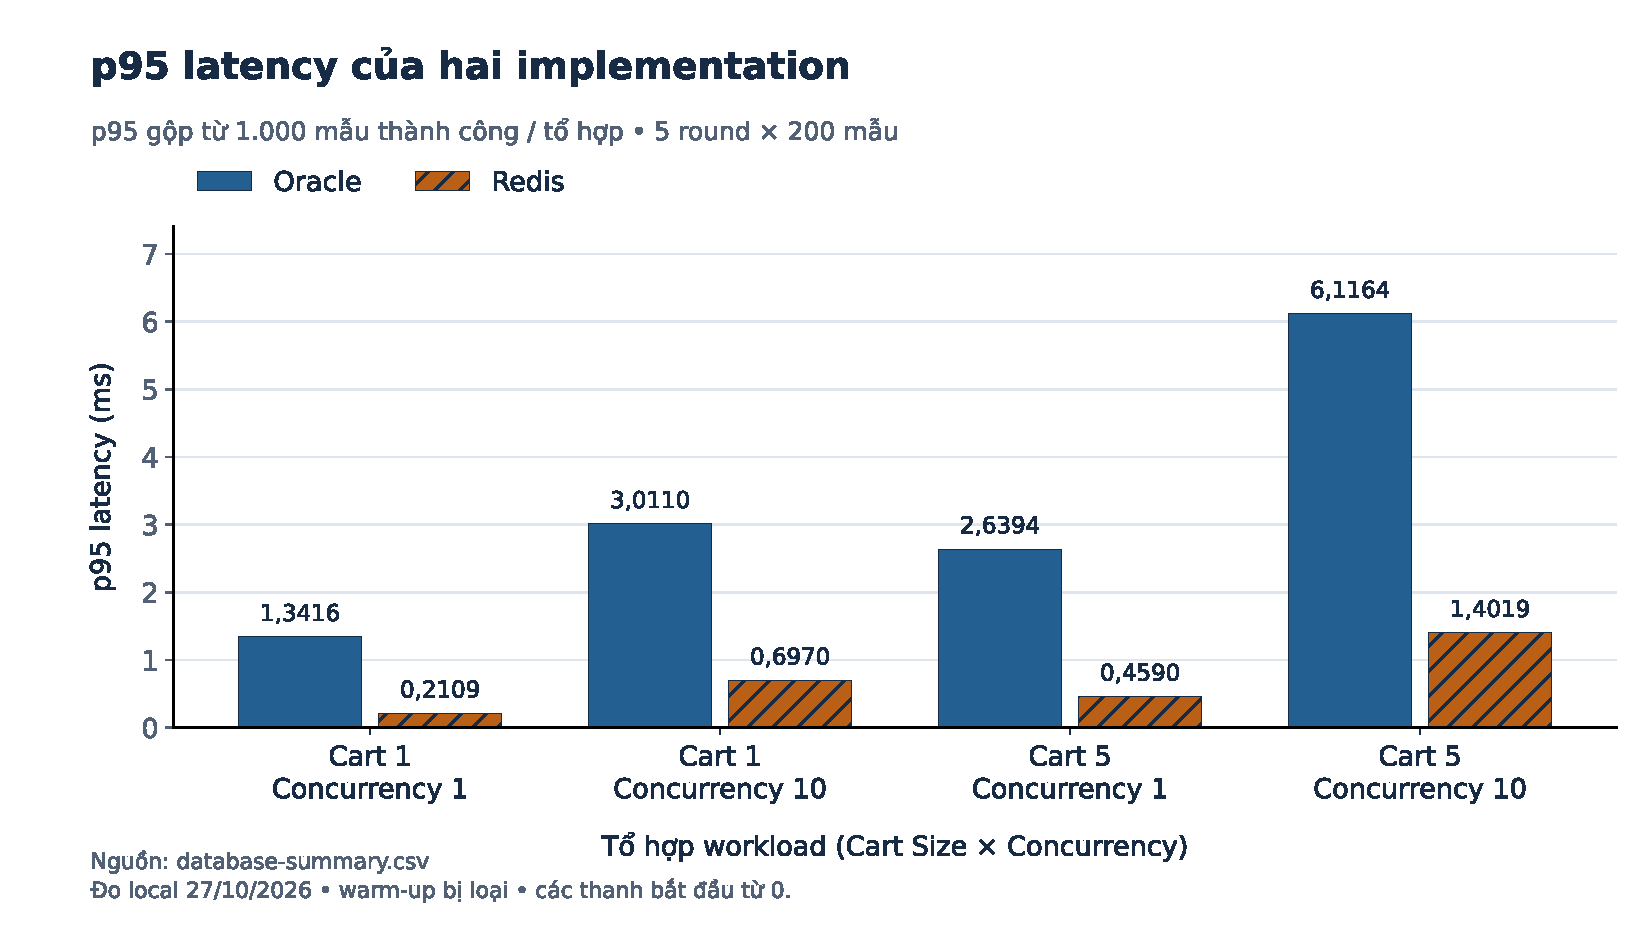
\includegraphics[width=\linewidth]{Pictures/Task_4/4.3-01-database-p95.pdf}
\caption[So sánh p95 latency Oracle–Redis theo Cart Size và Concurrency]{So sánh p95 latency Oracle–Redis theo Cart Size và Concurrency; dữ liệu từ bảng Database-level Benchmark, đơn vị ms.}\label{fig:tx-1}
\end{figure}
\begin{figure}[!htbp]
\centering
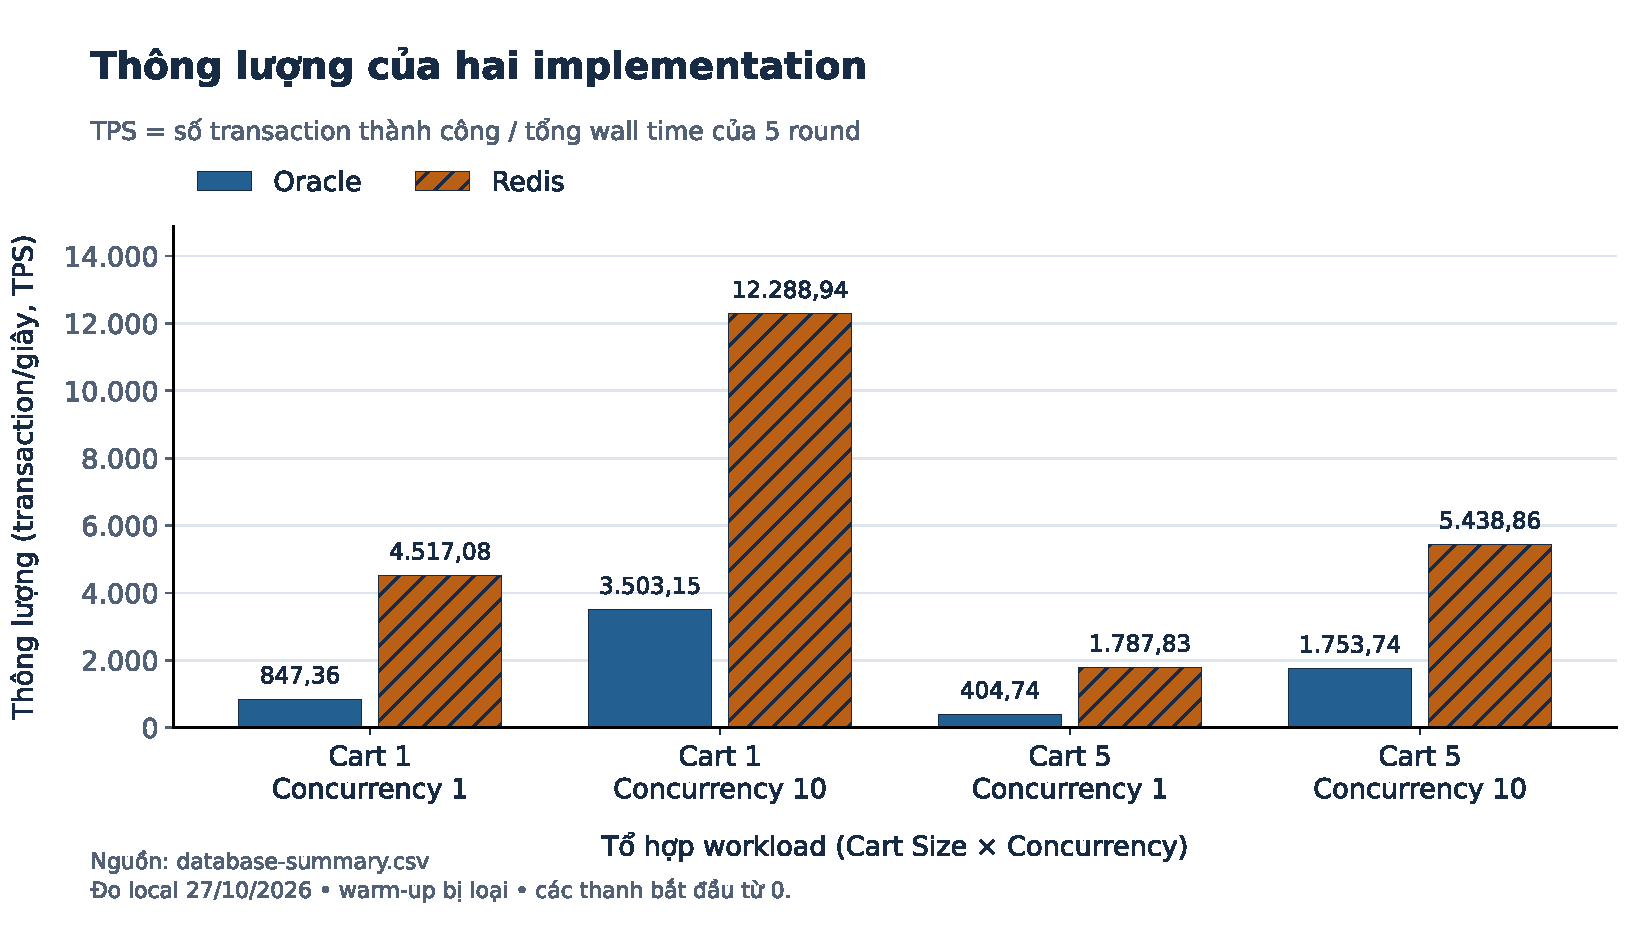
\includegraphics[width=\linewidth]{Pictures/Task_4/4.3-02-database-tps.pdf}
\caption[So sánh TPS Oracle–Redis theo bốn tổ hợp tải]{So sánh TPS Oracle–Redis theo bốn tổ hợp tải; dữ liệu từ bảng Database-level Benchmark.}\label{fig:tx-2}
\end{figure}
\textbf{Nhận xét kết quả.} Khi tăng Cart Size từ 1 lên 5, \textbf{p95 tăng và TPS giảm} ở cả hai implementation do một transaction phải xử lý nhiều dòng sản phẩm hơn. Khi tăng Concurrency từ 1 lên 10, \textbf{TPS tăng nhưng p95 cũng tăng}, phản ánh sự đánh đổi giữa thông lượng và thời gian xử lý từng giao dịch.

Redis có \textbf{p95 thấp hơn và TPS cao hơn trong cả bốn tổ hợp}. Ở Cart Size 5, Concurrency 10, Oracle đạt \textbf{6,1164 ms và 1.753,74 TPS}, trong khi Redis đạt \textbf{1,4019 ms và 5.438,86 TPS}. Kết quả này ghi nhận ưu thế của implementation Redis trong workload đã đo, nhưng chưa đủ để khẳng định Redis nhanh hơn Oracle đối với mọi transaction.

\begin{table}[!htbp]
\centering
\caption{Trung bình và độ lệch chuẩn của p95 qua năm round. Nguồn: \texttt{results/\allowbreak{}summary-\allowbreak{}20261027/\allowbreak{}database-\allowbreak{}summary.\allowbreak{}csv}.}\label{tab:tx-20}
\reporttablesetup
\begin{tabularx}{\linewidth}{|>{\hsize=0.65\hsize\linewidth=\hsize}L|>{\hsize=0.85\hsize\linewidth=\hsize}L|>{\hsize=1.25\hsize\linewidth=\hsize}L|>{\hsize=1.25\hsize\linewidth=\hsize}L|}
\hline
\rowcolor{ReportTableHead}
\reportheader{Cart Size} & \reportheader{Concurrency} & \reportheader{Oracle p95 TB \(\pm\) SD (ms)} & \reportheader{Redis p95 TB \(\pm\) SD (ms)} \\ \hline
1 & 1 & 1,2784 \(\pm\) 0,2425 & 0,1869 \(\pm\) 0,0451 \\ \hline
1 & 10 & 3,0004 \(\pm\) 0,1745 & 0,7042 \(\pm\) 0,0370 \\ \hline
5 & 1 & 2,6187 \(\pm\) 0,0733 & 0,4494 \(\pm\) 0,0388 \\ \hline
5 & 10 & 5,7613 \(\pm\) 0,5800 & 1,3381 \(\pm\) 0,2104 \\ \hline
\end{tabularx}
\end{table}
Chênh lệch giữa các round không đảo ngược xu hướng hiệu năng trên. Toàn bộ \textbf{8.000/8.000 transaction thành công}, không phát hiện invariant violation trong phạm vi hậu kiểm. Tuy nhiên, fixture chủ yếu độc lập giữa các worker, nên benchmark \textbf{chưa đo mức tranh chấp cao trên cùng sản phẩm}; khác biệt về schema, kết nối và durability cũng cần được xét khi diễn giải kết quả.

\txsubsection{Kết quả Application-level Benchmark}\label{sec:tx-3-3}
Phép đo HTTP sử dụng \textbf{k6 \(\rightarrow\) Vite proxy \(\rightarrow\) Spring Boot \(\rightarrow\) Oracle}, nhằm quan sát hiệu năng nghiệp vụ thực tế, \textbf{không so sánh Oracle với Redis ở tầng ứng dụng}. Một flow gồm đọc Cart, thêm 1 hoặc 5 sản phẩm, xem Checkout Preview, tạo Order, truy vấn danh sách/chi tiết Order và hủy Order. Do đó, \textbf{4.000 flow} tương ứng \textbf{36.000 HTTP request nghiệp vụ} (7 request/flow với Cart Size 1; 11 request/flow với Cart Size 5), không tính warm-up và login.

Bảng kết quả phân biệt \textbf{Checkout API} — riêng request tạo Order — với \textbf{Full Flow} — toàn bộ chuỗi thao tác nói trên.

\begin{table}[!htbp]
\centering
\caption{Kết quả Application-level Benchmark. Latency lấy từ các mẫu thành công; Flow/s tính theo số flow thành công trên tổng thời gian thực của năm round. Nguồn: \texttt{results/\allowbreak{}summary-\allowbreak{}20261027/\allowbreak{}http-\allowbreak{}summary.\allowbreak{}csv}.}\label{tab:tx-21}
\reporttablesetup
\scriptsize
\begin{tabularx}{\linewidth}{|>{\hsize=0.6\hsize\linewidth=\hsize}L|>{\hsize=1.05\hsize\linewidth=\hsize}L|>{\hsize=1.1\hsize\linewidth=\hsize}L|>{\hsize=1.1\hsize\linewidth=\hsize}L|>{\hsize=1.1\hsize\linewidth=\hsize}L|>{\hsize=1.1\hsize\linewidth=\hsize}L|>{\hsize=0.95\hsize\linewidth=\hsize}L|}
\hline
\rowcolor{ReportTableHead}
\reportheader{Cart Size} & \reportheader{Concurrency} & \reportheader{Checkout p50 (ms)} & \reportheader{Checkout p95 (ms)} & \reportheader{Full Flow p50 (ms)} & \reportheader{Full Flow p95 (ms)} & \reportheader{Flow/s} \\ \hline
1 & 1 & 2,9084 & 4,0406 & 14 & 18 & 68,34 \\ \hline
1 & 10 & 6,5273 & 8,9241 & 33 & 42 & 296,08 \\ \hline
5 & 1 & 4,9161 & 10,2897 & 30 & 62 & 27,73 \\ \hline
5 & 10 & 11,1444 & 14,7888 & 61 & 74 & 157,57 \\ \hline
\end{tabularx}
\end{table}
\begin{figure}[!htbp]
\centering
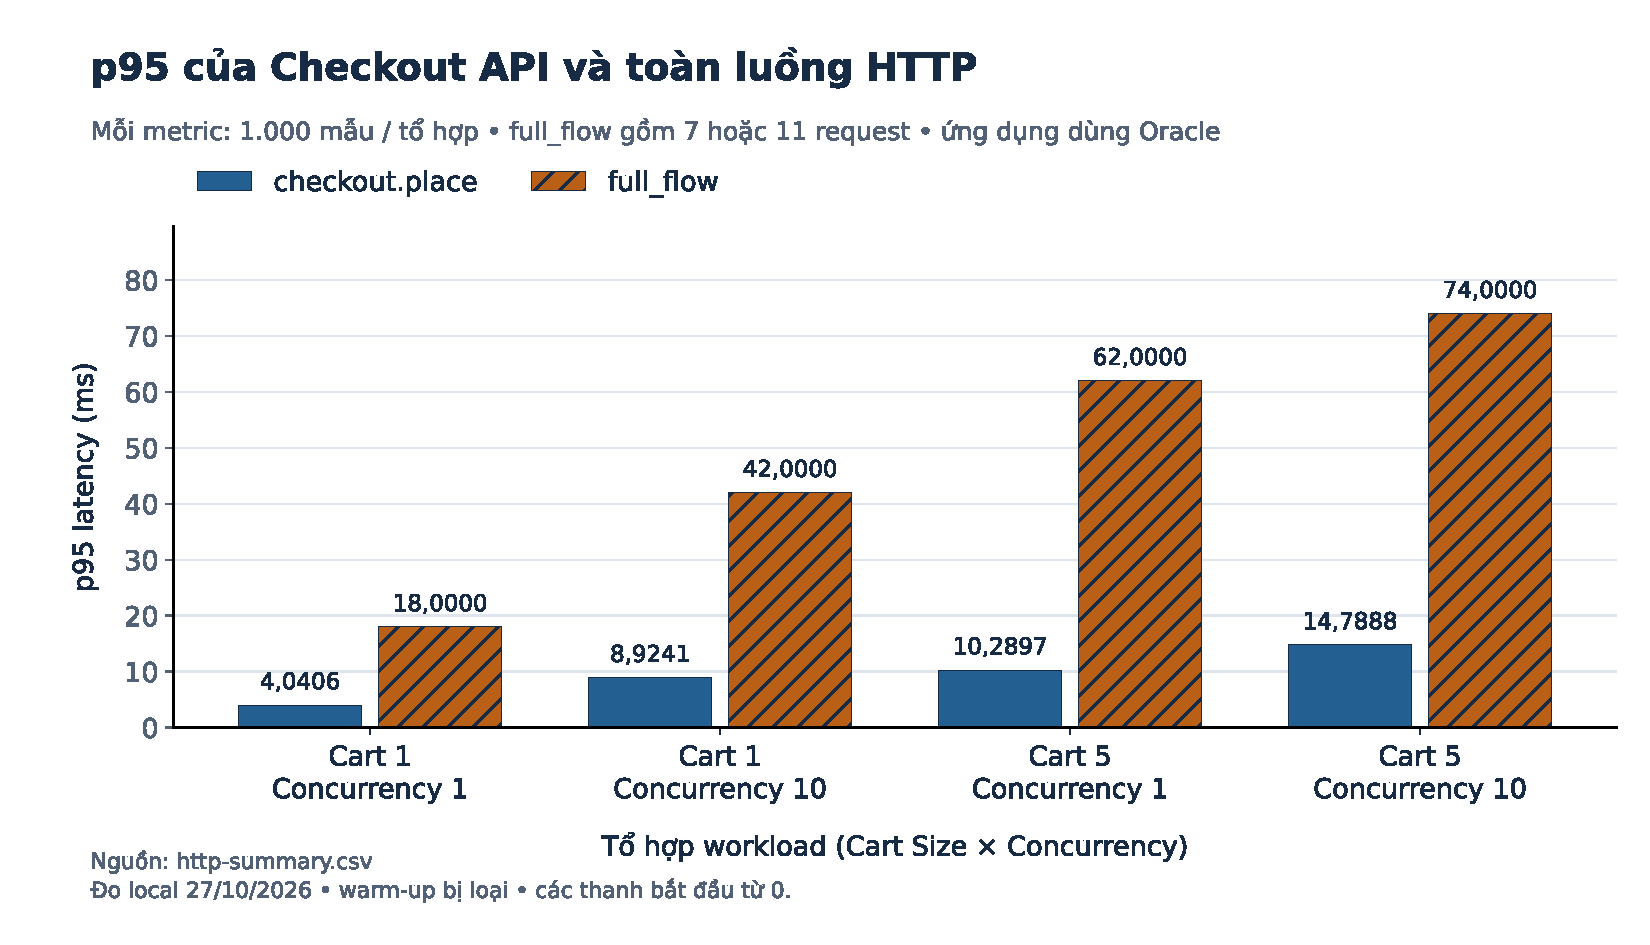
\includegraphics[width=\linewidth]{Pictures/Task_4/4.3-03-http-p95.pdf}
\caption[So sánh p95 Checkout API và Full Flow theo Cart Size/\allowbreak{}Concurrency]{So sánh p95 Checkout API và Full Flow theo Cart Size/\allowbreak{}Concurrency; dữ liệu từ bảng HTTP benchmark, đơn vị ms.}\label{fig:tx-3}
\end{figure}
\textbf{Nhận xét kết quả.} Khi Cart Size tăng từ 1 lên 5 ở Concurrency 1, Checkout p95 tăng từ \textbf{4,0406 lên 10,2897 ms}, Full Flow p95 tăng từ \textbf{18 lên 62 ms}. Nguyên nhân là Checkout phải xử lý nhiều sản phẩm và flow có thêm các request thêm Cart Item. Khi Concurrency tăng từ 1 lên 10, throughput tăng ở cả hai Cart Size (tương ứng \textbf{68,34 \(\rightarrow\) 296,08} và \textbf{27,73 \(\rightarrow\) 157,57 flow/s}), nhưng latency cũng tăng.

\textbf{Full Flow p95 cao hơn Checkout p95} vì chứa nhiều bước nghiệp vụ; không thể lấy chênh lệch hai phân vị làm chi phí chính xác của những API còn lại. Cả \textbf{4.000/4.000 flow hoàn tất}, không phát hiện invariant violation theo hậu kiểm. Kết quả cho thấy backend Oracle vận hành được dưới các mức tải đã thử, nhưng môi trường local và việc chưa tạo tranh chấp mạnh không đủ để suy ra hiệu năng production. \textbf{TPS database và Flow/s HTTP không thể so sánh trực tiếp} do khác đơn vị công việc.

\txsubsection{Đối chiếu tổng hợp và lựa chọn DBMS phù hợp}\label{sec:tx-3-4}
Từ các thí nghiệm về ACID và kết quả benchmark, có thể nhận thấy Oracle và Redis đều cung cấp những cơ chế hỗ trợ xử lý transaction, nhưng khác nhau đáng kể về phạm vi bảo đảm, cách kiểm soát lỗi và hiệu năng của các cách triển khai được khảo sát.

Bảng~\ref{tab:tx-22} tổng hợp những khác biệt có ảnh hưởng trực tiếp đến việc lựa chọn DBMS.

\begin{table}[!htbp]
\centering
\caption{Tổng hợp kết quả nghiên cứu Transaction trên Oracle và Redis.}\label{tab:tx-22}
\reporttablesetup
\begin{tabularx}{\linewidth}{|>{\hsize=0.65\hsize\linewidth=\hsize}L|>{\hsize=1.175\hsize\linewidth=\hsize}L|>{\hsize=1.175\hsize\linewidth=\hsize}L|}
\hline
\rowcolor{ReportTableHead}
\reportheader{Tiêu chí} & \reportheader{Oracle} & \reportheader{Redis} \\ \hline
\textbf{Atomicity} & Hỗ trợ COMMIT, ROLLBACK và SAVEPOINT; cho phép hoàn tác các thay đổi chưa commit trên nhiều bảng (A1, A3, D1). & MULTI/EXEC và Lua thực thi không bị command khác chen ngang, nhưng không tự hoàn tác những ghi thành công trước lỗi runtime (A4, A5). \\ \hline
\textbf{Consistency} & DBMS trực tiếp thực thi các constraint như PK, FK, UNIQUE và CHECK (C1, A2). & Các ràng buộc nghiệp vụ giữa những key phải được kiểm tra và bảo vệ trong đường ghi, chẳng hạn Lua guarded Checkout (C2). \\ \hline
\textbf{Isolation và Concurrency} & READ COMMITTED, row lock và SELECT FOR UPDATE hỗ trợ kiểm soát truy cập đồng thời; có cơ chế phát hiện deadlock (B1–B3). & Atomic command, WATCH và Lua hỗ trợ xử lý xung đột; cần lựa chọn cơ chế phù hợp với từng thao tác (B4, B5). \\ \hline
\textbf{Durability} & Sử dụng Redo Log và cơ chế phục hồi transaction. & Hỗ trợ RDB/AOF; môi trường khảo sát sử dụng AOF \texttt{everysec}. Chưa thực hiện crash-recovery benchmark để so sánh trực tiếp. \\ \hline
\textbf{Hiệu năng} & Có latency cao hơn và TPS thấp hơn trong workload database đã đo. & Có latency thấp hơn và TPS cao hơn trong cùng các tổ hợp khảo sát, nhưng hai implementation chưa tương đương hoàn toàn về ràng buộc và chi phí thực thi. \\ \hline
\end{tabularx}
\end{table}
\paragraph*{Đánh giá và quyết định đối với Oracle}

Trong bối cảnh thương mại điện tử, các nghiệp vụ Checkout, tạo đơn hàng và quản lý tồn kho đòi hỏi nhiều thao tác dữ liệu có quan hệ chặt chẽ. Oracle được đánh giá phù hợp với các yêu cầu này dựa trên ba cơ sở:

\begin{enumerate}[leftmargin=*,itemsep=2pt,topsep=4pt]
\item
\textbf{Khả năng quản lý transaction nhiều bước:} Hỗ trợ thực hiện và hoàn tác nhiều thay đổi trên các bảng trong cùng transaction, được kiểm chứng qua D1.

\item
\textbf{Bảo vệ tính toàn vẹn dữ liệu:} Các constraint được thực thi tại DBMS, giúp bảo vệ dữ liệu trên nhiều đường ghi khác nhau (A2, C1).

\item
\textbf{Kiểm soát truy cập đồng thời:} Row-level locking và SELECT FOR UPDATE hỗ trợ bảo vệ thao tác đọc–quyết định–ghi trong những nghiệp vụ có tranh chấp (B1–B3).

\end{enumerate}
\textbf{Quyết định:} Nhóm lựa chọn \textbf{Oracle làm nguồn dữ liệu chính (source of truth)} cho ShopFlash. Các nghiệp vụ Normal Checkout và Order Cancellation được thiết kế thực hiện trong Oracle transaction để bảo đảm việc tạo/cập nhật Order, Order Items, Inventory và Cart được xác nhận hoặc hoàn tác nhất quán. Dữ liệu giao dịch và kết quả mua Flash Sale thành công cũng được lưu trữ chính thức tại Oracle.

\paragraph*{Đánh giá và quyết định đối với Redis}

Redis thể hiện ưu thế về thời gian xử lý trong benchmark và cung cấp những cơ chế phù hợp với các thao tác có phạm vi dữ liệu hẹp, yêu cầu xử lý đồng thời cao:

\begin{enumerate}[leftmargin=*,itemsep=2pt,topsep=4pt]
\item
\textbf{Atomic Command:} Các thao tác như HINCRBY cho phép cập nhật bộ đếm nguyên tử mà không cần triển khai khóa riêng cho từng phép tăng/giảm (B4).

\item
\textbf{WATCH và Lua:} Hỗ trợ phát hiện xung đột hoặc kết hợp kiểm tra và cập nhật nhiều key trong một lần thực thi, phù hợp với việc kiểm soát quota (B4, B5).

\item
\textbf{Giới hạn transaction:} Không có full rollback tương đương Oracle khi phát sinh lỗi runtime sau ghi, nên cần validation trước ghi và cơ chế xử lý lỗi phù hợp (A5, C2).

\end{enumerate}
\textbf{Quyết định:} Nhóm lựa chọn \textbf{Redis cho Flash Sale runtime}, bao gồm kiểm soát quota, giới hạn mua theo người dùng và reservation tạm thời bằng Lua. Ngoài ra, Redis được sử dụng cho các dữ liệu dẫn xuất phục vụ tìm kiếm và thống kê, không thay thế Oracle làm nguồn dữ liệu giao dịch chính.

\paragraph*{Kết luận lựa chọn}

ShopFlash được thiết kế theo hướng kết hợp hai DBMS: \textbf{Oracle bảo đảm tính đúng đắn của dữ liệu giao dịch chính, Redis hỗ trợ các thao tác runtime cần tốc độ cao}. Đây là lựa chọn phù hợp với yêu cầu nghiệp vụ và những cơ chế đã nghiên cứu.

\endgroup

% !TeX root = ../../main.tex
\subsection{Concurrency Control}\label{sec:cc}
% Nội dung do thành viên phụ trách Concurrency control bổ sung.

% !TeX root = ../../main.tex
\subsection{Data Backup \& Recovery}\label{sec:backup}
\begingroup
% Đánh số bảng/hình theo mục (2.x.y), giống Transaction.
\setcounter{table}{0}\setcounter{figure}{0}
\renewcommand{\thetable}{\thesubsection.\arabic{table}}
\renewcommand{\thefigure}{\thesubsection.\arabic{figure}}
\renewcommand{\theHtable}{\thesubsection.\arabic{table}}
\renewcommand{\theHfigure}{\thesubsection.\arabic{figure}}
\subsubsection{Mục tiêu và phạm vi}

Phân hệ sao lưu và phục hồi được thiết kế nhằm đảm bảo khả năng khôi phục toàn vẹn dữ liệu hệ thống ShopFlash khi xảy ra sự cố phần cứng hoặc thảm họa dữ liệu. Phạm vi thực nghiệm không chỉ dừng ở các bảng danh mục sản phẩm mà mở rộng ra toàn bộ dữ liệu nghiệp vụ của schema \texttt{SHOP} trên Oracle Database và toàn bộ keyspace trên Redis.

Mục tiêu chính của thử nghiệm nhằm: (i) kiểm chứng tính toàn vẹn và khả năng phục hồi đồng thời của cả hai hệ quản trị cơ sở dữ liệu về trạng thái baseline chuẩn sau sự cố; (ii) đo đạc chi phí thời gian kỹ thuật thực tế cho thao tác backup và recovery; và (iii) đánh giá thực nghiệm tác động của các chế độ persistence trong Redis nhằm chọn ra cấu hình phù hợp nhất cho ShopFlash.

\subsubsection{Cơ sở lý thuyết về sao lưu và phục hồi}

\paragraph{Cơ chế sao lưu và phục hồi của Oracle Database}

Oracle cung cấp các giải pháp sao lưu từ cấp độ vật lý (RMAN) đến cấp độ logic (Oracle Data Pump) \cite{oracleDataPump}. Trong mô hình ứng dụng quy mô vừa như ShopFlash, Oracle Data Pump (\texttt{expdp}/\texttt{impdp}) là công cụ sao lưu logic hiệu quả, cho phép trích xuất toàn bộ định nghĩa đối tượng (schema metadata) và dữ liệu dòng dưới dạng các tập tin dump đĩa cứng. Khi phục hồi, Data Pump tự động tái tạo lại cấu trúc bảng, chỉ mục, ràng buộc toàn vẹn và nạp lại dữ liệu với hiệu năng cao nhờ cơ chế Direct Path I/O \cite{oracleDataPump}.

\paragraph{Cơ chế Persistence của Redis}

Redis hỗ trợ hai cơ chế lưu trữ bền vững độc lập hoặc kết hợp \cite{redisPersistence}:
\begin{itemize}[label=--]
    \item \textbf{RDB (Redis Database Backup):} Tạo ảnh chụp snapshot toàn bộ bộ nhớ tại một thời điểm và ghi xuống đĩa dưới dạng file nhị phân nén. RDB có ưu điểm kích thước gọn, tốc độ nạp lại cực nhanh khi khởi động, nhưng có nguy cơ mất dữ liệu phát sinh giữa hai lần chụp snapshot \cite{redisPersistence}.
    \item \textbf{AOF (Append-Only File):} Ghi lại toàn bộ các lệnh ghi (write operations) vào nhật ký theo thời gian thực. AOF cung cấp tính bền vững cao hơn thông qua các chính sách đồng bộ đĩa (\texttt{appendfsync}): \texttt{always} (fsync mỗi lệnh ghi), \texttt{everysec} (fsync mỗi giây) hoặc \texttt{no} (giao cho OS). Khi khởi động, Redis ưu tiên đọc file AOF để tái tạo trạng thái dữ liệu \cite{redisPersistence}.
\end{itemize}

\subsubsection{Thiết kế lưu trữ sao lưu trong ShopFlash}

Nhằm đảm bảo tính đồng bộ giữa hai cơ sở dữ liệu, mỗi lượt backup tạo ra một gói sao lưu chứa Data Pump export cho schema \texttt{SHOP} và RDB snapshot cho Redis keyspace, kèm file manifest lưu mã SHA-256 để kiểm tra tính toàn vẹn.

Khi thực hiện phục hồi, script điều phối tiến hành import Data Pump vào Oracle để đưa dữ liệu nghiệp vụ gốc về trạng thái chuẩn. Đối với Redis, do hệ thống bật AOF ở chế độ \texttt{appendfsync everysec}, file RDB snapshot sẽ được nạp trong một container cô lập tạm thời để khởi tạo lại file AOF trước khi đưa service vào vận hành, tránh việc file AOF cũ đè lên dữ liệu vừa phục hồi \cite{redisPersistence}.

\begin{table}[H]
    \centering
    \caption{Tóm tắt cơ chế phục hồi dữ liệu trong ShopFlash}
    \label{tab:bk-backup-artifacts}
    \begin{tabularx}{\textwidth}{@{}p{0.18\textwidth}p{0.25\textwidth}XX@{}}
        \toprule
        Nguồn & Artifact & Cơ chế phục hồi & Mục tiêu bảo vệ \\
        \midrule
        Oracle & Data Pump export (\texttt{.dmp}) & Import logic qua Data Pump; giữ nguyên cấu trúc schema hiện có & Dữ liệu nghiệp vụ gốc, quan hệ và các ràng buộc toàn vẹn \\
        Redis & RDB snapshot (\texttt{.rdb}) & Nạp RDB và tái tạo file AOF trước khi khởi chạy service & Product projection và trạng thái runtime \\
        \bottomrule
    \end{tabularx}
\end{table}

\subsubsection{Đánh giá thực nghiệm}

Thử nghiệm được thực hiện trên dataset chuẩn gồm 100 Category, 1\,000 Product, 1\,000 bản ghi ProductInventory và 1\,000 Redis document \texttt{product:*}.

\paragraph{Thử nghiệm thời gian sao lưu và phục hồi}

\noindent\textbf{Phương pháp}\par
Quy trình thực nghiệm bao gồm 5 lượt tạo backup độc lập để đo thời gian xuất dữ liệu và kích thước artifact. Thời gian tạo backup được tính trực tiếp từ lúc khởi chạy xuất dữ liệu đến khi hoàn tất tính mã SHA-256.

Sau đó, quy trình giả lập thảm họa được thực thi bằng cách xóa sạch toàn bộ dữ liệu nghiệp vụ của Oracle và toàn bộ keyspace Redis. Script phục hồi tiến hành kiểm tra checksum SHA-256, nạp lại dữ liệu cho hai hệ thống và đối chiếu số lượng bản ghi (checkpoint) so với baseline ban đầu.

\noindent\textbf{Kết quả và phân tích}\par
Kích thước file backup duy trì độ ổn định cao qua các lượt chạy (Oracle .dmp đạt 1\,355\,776 bytes, Redis .rdb đạt 190\,018 bytes). Thời gian hoàn thành thao tác sao lưu toàn hệ thống trung bình là 62.902 giây với độ lệch chuẩn 2.742 giây (Bảng~\ref{tab:bk-backup-duration}).

\begin{table}[H]
    \centering
    \caption{Thời gian tạo backup toàn hệ thống (5 lượt thử nghiệm)}
    \label{tab:bk-backup-duration}
    \begin{tabular}{@{}crrr@{}}
        \toprule
        Lượt & Oracle Data Pump (bytes) & Redis RDB (bytes) & Thời gian tạo (s) \\
        \midrule
        1 & 1\,355\,776 & 190\,018 & 63.026 \\
        2 & 1\,355\,776 & 190\,018 & 67.478 \\
        3 & 1\,355\,776 & 190\,018 & 60.923 \\
        4 & 1\,355\,776 & 190\,018 & 60.679 \\
        5 & 1\,355\,776 & 190\,018 & 62.402 \\
        \midrule
        Trung bình & 1\,355\,776 & 190\,018 & 62.902 \\
        Độ lệch chuẩn & 0 & 0 & 2.742 \\
        \bottomrule
    \end{tabular}
\end{table}

Trước khi restore, mã SHA-256 của file \texttt{.dmp} và \texttt{dump.rdb} được đối chiếu và đều khớp tuyệt đối với manifest. Kết quả Bảng~\ref{tab:bk-recovery-duration} cho thấy 100\% các lượt thử nghiệm khôi phục thành công. Thời gian phục hồi trung bình của Oracle là 23.710 giây và Redis là 9.186 giây; tổng thời gian phục hồi kỹ thuật trung bình là 32.895 giây.

\begin{table}[H]
    \centering
    \caption{Kết quả đo thời gian phục hồi dữ liệu (5 lượt thử nghiệm)}
    \label{tab:bk-recovery-duration}
    \begin{tabular}{@{}crrrcc@{}}
        \toprule
        Lượt & Oracle (s) & Redis (s) & Tổng thời gian (s) & Oracle khớp & Redis khớp \\
        \midrule
        1 & 25.901 & 8.946 & 34.847 & Có & Có \\
        2 & 24.676 & 8.848 & 33.524 & Có & Có \\
        3 & 23.539 & 9.246 & 32.785 & Có & Có \\
        4 & 22.678 & 9.642 & 32.320 & Có & Có \\
        5 & 21.755 & 9.246 & 31.001 & Có & Có \\
        \midrule
        Trung bình & 23.710 & 9.186 & 32.895 & Có & Có \\
        Độ lệch chuẩn & 1.632 & 0.311 & 1.426 & -- & -- \\
        \bottomrule
    \end{tabular}
\end{table}

Cả hai hệ thống sau phục hồi đều khôi phục trọn vẹn số lượng bản ghi về đúng trạng thái baseline ban đầu (Bảng~\ref{tab:bk-recovery-checkpoint}).

\begin{table}[H]
    \centering
    \caption{Trạng thái checkpoint bản ghi trong quy trình phục hồi dữ liệu}
    \label{tab:bk-recovery-checkpoint}
    \begin{tabularx}{\textwidth}{@{}Xrrrrr@{}}
        \toprule
        Trạng thái kiểm tra & Category & Product & Inventory & Redis key & \texttt{product:*} \\
        \midrule
        Trước khi mất dữ liệu (Baseline) & 100 & 1\,000 & 1\,000 & 1\,000 & 1\,000 \\
        Sau khi giả lập sự cố & 0 & 0 & 0 & 0 & 0 \\
        Sau khi restore Oracle & 100 & 1\,000 & 1\,000 & 0 & 0 \\
        Sau khi restore Redis & 100 & 1\,000 & 1\,000 & 1\,000 & 1\,000 \\
        \bottomrule
    \end{tabularx}
\end{table}

\paragraph{Thử nghiệm đánh giá hiệu năng các chế độ Persistence của Redis}

\noindent\textbf{Phương pháp}\par
Sử dụng công cụ \texttt{redis-benchmark} \cite{redisBenchmark} thực thi 100\,000 lệnh \texttt{SET} và 100\,000 lệnh \texttt{GET} trên 50 client đồng thời (value size 256 bytes) nhằm đo lường throughput (ops/sec) và độ trễ p95 của Redis ở 3 cấu hình AOF khác nhau: tắt AOF, AOF \texttt{everysec} và AOF \texttt{always}.

\noindent\textbf{Kết quả và phân tích}\par
Số liệu thu được từ bảng~\ref{tab:bk-redis-persistence-benchmark} thể hiện rõ sự khác biệt về chi phí ghi giữa các chế độ đồng bộ đĩa.

\begin{table}[H]
    \centering
    \caption{So sánh hiệu năng theo chế độ Persistence của Redis}
    \label{tab:bk-redis-persistence-benchmark}
    \begin{tabularx}{\textwidth}{@{}Xrrrr@{}}
        \toprule
        Chế độ AOF & SET (ops/s) & SET p95 (ms) & GET (ops/s) & GET p95 (ms) \\
        \midrule
        AOF tắt (\texttt{appendonly no}) & 205\,127.55 & 0.180 & 206\,017.96 & 0.172 \\
        AOF \texttt{everysec} & 227\,426.15 & 0.186 & 202\,603.07 & 0.170 \\
        AOF \texttt{always} & 8\,493.02 & 7.764 & 202\,353.34 & 0.183 \\
        \bottomrule
    \end{tabularx}
\end{table}

Chế độ \texttt{appendfsync always} ép Redis phải thực hiện fsync xuống đĩa ở mỗi lệnh ghi, khiến throughput ghi giảm mạnh xuống chỉ còn 8\,493 ops/s và độ trễ p95 tăng lên 7.764 ms (gấp hơn 40 lần). Ngược lại, chế độ \texttt{everysec} đạt throughput ghi tương đương với khi tắt AOF hoàn toàn, trong khi hiệu năng đọc (GET) không bị ảnh hưởng bởi chế độ AOF.

\subsubsection{Đánh giá tổng hợp và định hướng sử dụng DBMS}

Từ kết quả thực nghiệm sao lưu và phục hồi, kiến trúc ShopFlash rút ra các kết luận định hướng vận hành:

\begin{itemize}[label=--]
    \item \textbf{Khả năng phục hồi sự cố:} Sự kết hợp giữa Oracle Data Pump và Redis RDB snapshot đảm bảo khôi phục 100\% trạng thái hệ thống sau thảm họa dữ liệu với tổng thời gian kỹ thuật chỉ khoảng 33 giây trên tập dữ liệu thử nghiệm.
    \item \textbf{Cấu hình Persistence tối ưu cho Redis:} Cấu hình \texttt{appendonly yes} kết hợp \texttt{appendfsync everysec} là lựa chọn tối ưu cho môi trường production của ShopFlash. Cấu hình này giúp cân bằng hoàn hảo giữa hiệu năng truy vấn cực cao của bộ nhớ trong và mức độ an toàn dữ liệu (giới hạn nguy cơ mất dữ liệu tối đa trong 1 giây khi xảy ra sự cố đột ngột), tránh được sụt giảm hiệu năng nghiêm trọng như chế độ \texttt{always}.
\end{itemize}
\endgroup


\clearpage
\section{HIỆN THỰC ỨNG DỤNG VÀ KẾT LUẬN}\label{sec:implementation}
\begingroup
\setstretch{1.15}
\fontsize{12}{16}\selectfont
\clubpenalty=10000
\widowpenalty=10000
% !TeX root = ../../main.tex
% Sáu ảnh gốc do người dùng cung cấp, chỉ đổi tên.
% Ảnh Flash Sale (client-flash-*, admin-flash-sales) do người phụ trách Concurrency (2.5) bổ sung,
% chụp ngày 16/11/2026. Chỗ bổ sung báo cáo/thống kê phía Admin vẫn giữ nguyên.

\subsection{Các chức năng đã hiện thực}\label{sec:implemented-features}

Bên cạnh việc nghiên cứu và so sánh Oracle với Redis, nhóm xây dựng ứng dụng thương mại điện tử ShopFlash nhằm vận dụng các cơ chế DBMS vào những nghiệp vụ cụ thể. Hệ thống cung cấp giao diện cho khách hàng, quản trị viên và các công cụ hỗ trợ quá trình thực nghiệm.

Các chức năng được tổ chức thành bốn nhóm chính:

\begin{table}[!htbp]
\centering
\caption{Tổng hợp các nhóm chức năng chính của ShopFlash.}\label{tab:impl-features}
\reporttablesetup
\begin{tabularx}{\linewidth}{|P{4cm}|L|}
\hline
\rowcolor{ReportTableHead}
\reportheader{Nhóm chức năng} & \reportheader{Nội dung hiện thực} \\ \hline
\textbf{Quản lý và tìm kiếm sản phẩm} & Quản lý danh mục, sản phẩm, tồn kho; tìm kiếm, lọc, sắp xếp và xem thông tin sản phẩm. \\ \hline
\textbf{Giỏ hàng và đơn hàng} & Thêm sản phẩm, điều chỉnh số lượng, lựa chọn sản phẩm đặt hàng, thực hiện Checkout, xem và quản lý đơn hàng. \\ \hline
\textbf{Flash Sale} & Quản lý chương trình khuyến mãi, kiểm soát quota và giới hạn mua, giữ suất tạm thời và đặt hàng Flash Sale. \\ \hline
\textbf{Báo cáo và thống kê} & Truy vấn doanh thu, thông tin sản phẩm và khách hàng; hỗ trợ các nguồn dữ liệu Oracle, Redis và cache theo từng chức năng. \\ \hline
\end{tabularx}
\end{table}


Ngoài các chức năng nghiệp vụ, hệ thống còn tích hợp những giao diện thực nghiệm và công cụ hỗ trợ quản trị cơ sở dữ liệu. Các thành phần này giúp nhóm thao tác, quan sát và kiểm chứng các cơ chế được nghiên cứu tại Phần 2.

\subsection{Minh họa và đánh giá ứng dụng}\label{sec:application-evaluation}

Các chức năng của ShopFlash được minh họa thông qua những màn hình và luồng nghiệp vụ tiêu biểu. Phần này tập trung vào khả năng tương tác và kết quả vận hành từ góc nhìn người dùng, trong khi các cơ chế kỹ thuật và kết quả thực nghiệm DBMS được trình bày tại Phần 2.

\subsubsection*{A. Giao diện phía khách hàng (Client)}

\paragraph*{Nhóm chức năng khám phá và tìm kiếm sản phẩm}

Giao diện trang chủ cung cấp điểm truy cập chính đến danh mục sản phẩm, chức năng tìm kiếm và các chương trình Flash Sale. Người dùng có thể duyệt những sản phẩm đang được bán hoặc chuyển trực tiếp đến trang danh sách sản phẩm để thực hiện tìm kiếm chi tiết.

\begin{figure}[!htbp]
\centering
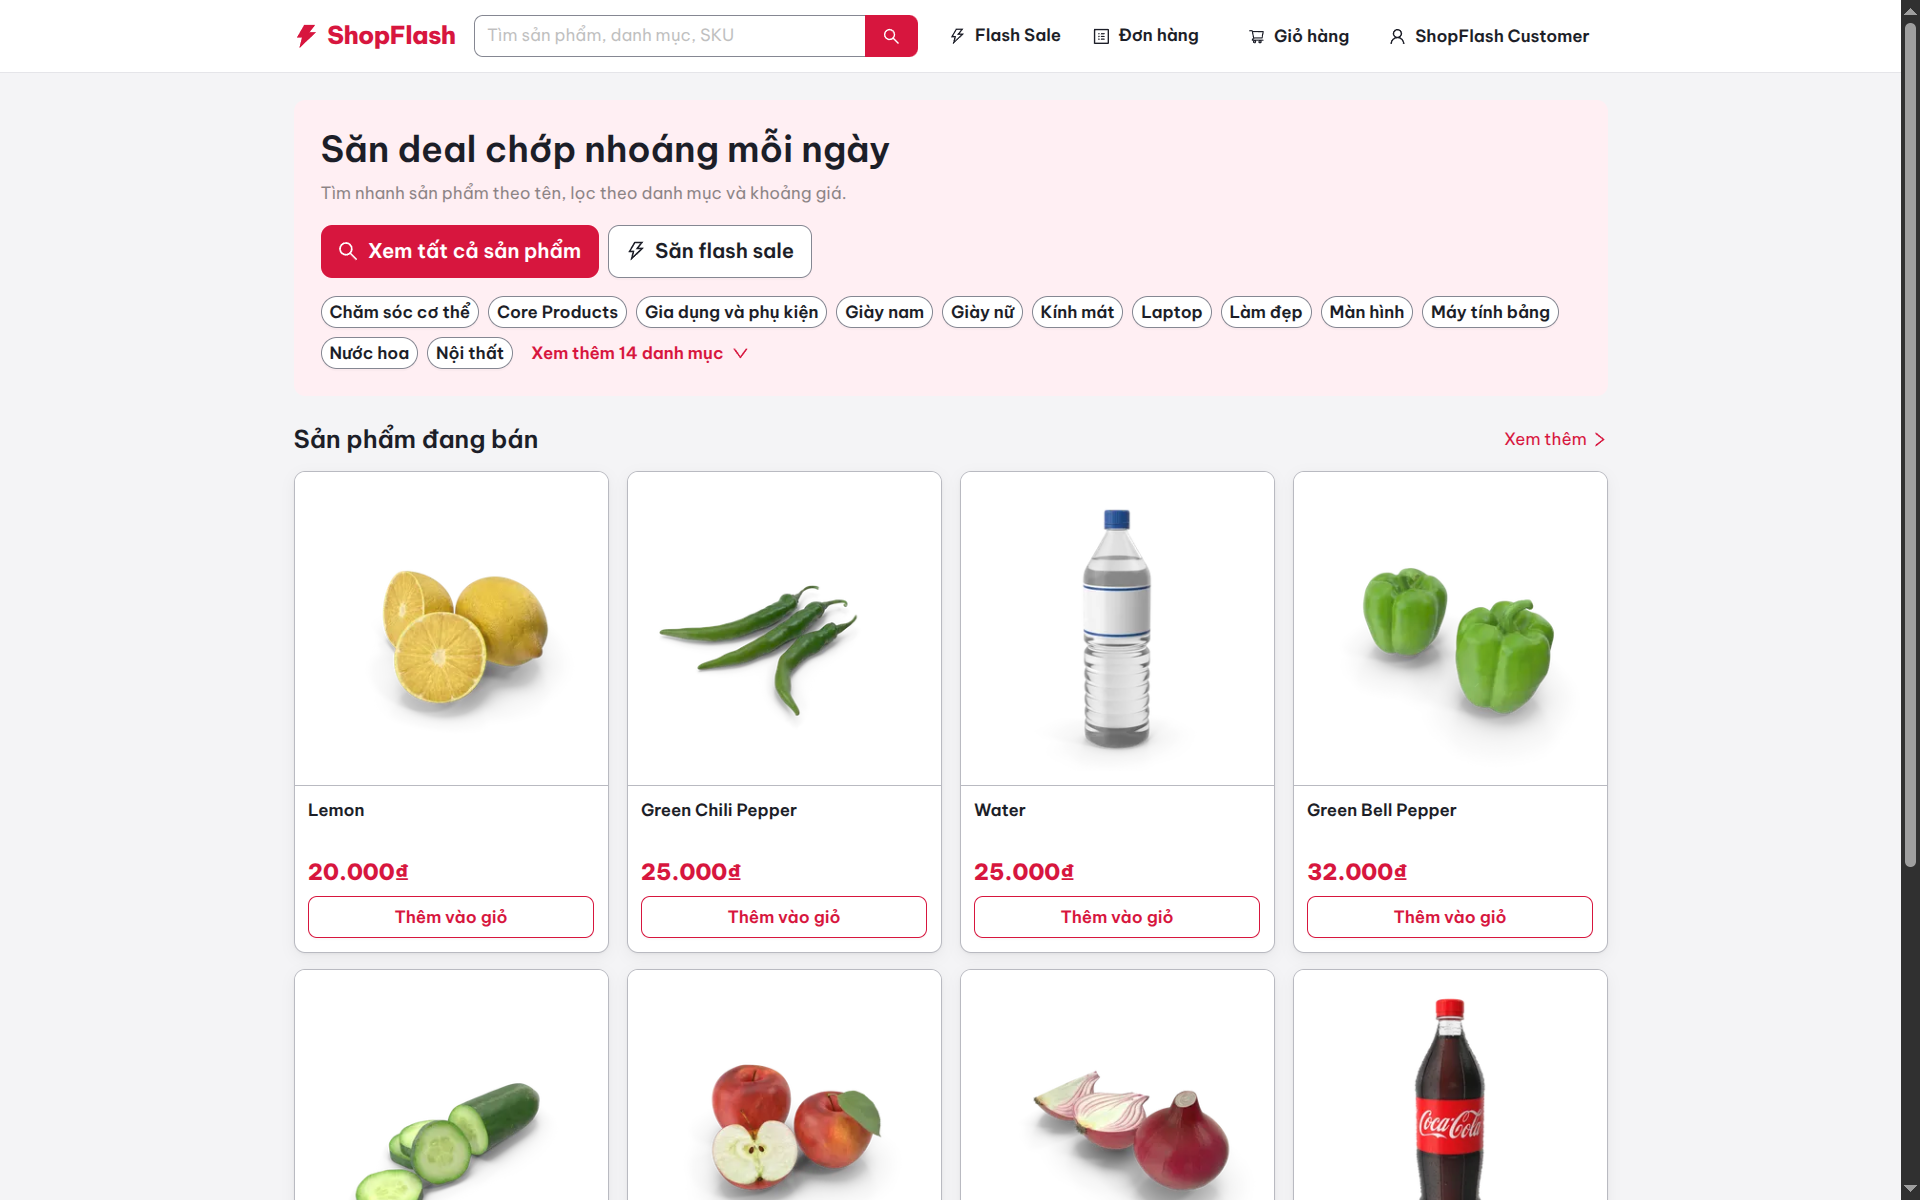
\includegraphics[width=\linewidth]{Pictures/Section_3/client-home.png}
\caption{Giao diện trang chủ ShopFlash với danh mục và danh sách sản phẩm đang bán.}\label{fig:impl-client-home}
\end{figure}


Trang danh sách sản phẩm hỗ trợ tìm kiếm, lọc theo danh mục, khoảng giá và sắp xếp theo giá. Ở thời điểm minh họa, hệ thống hiển thị 194 sản phẩm cùng bộ lọc và các thông tin cơ bản như hình ảnh, tên và giá bán.

\begin{figure}[!htbp]
\centering
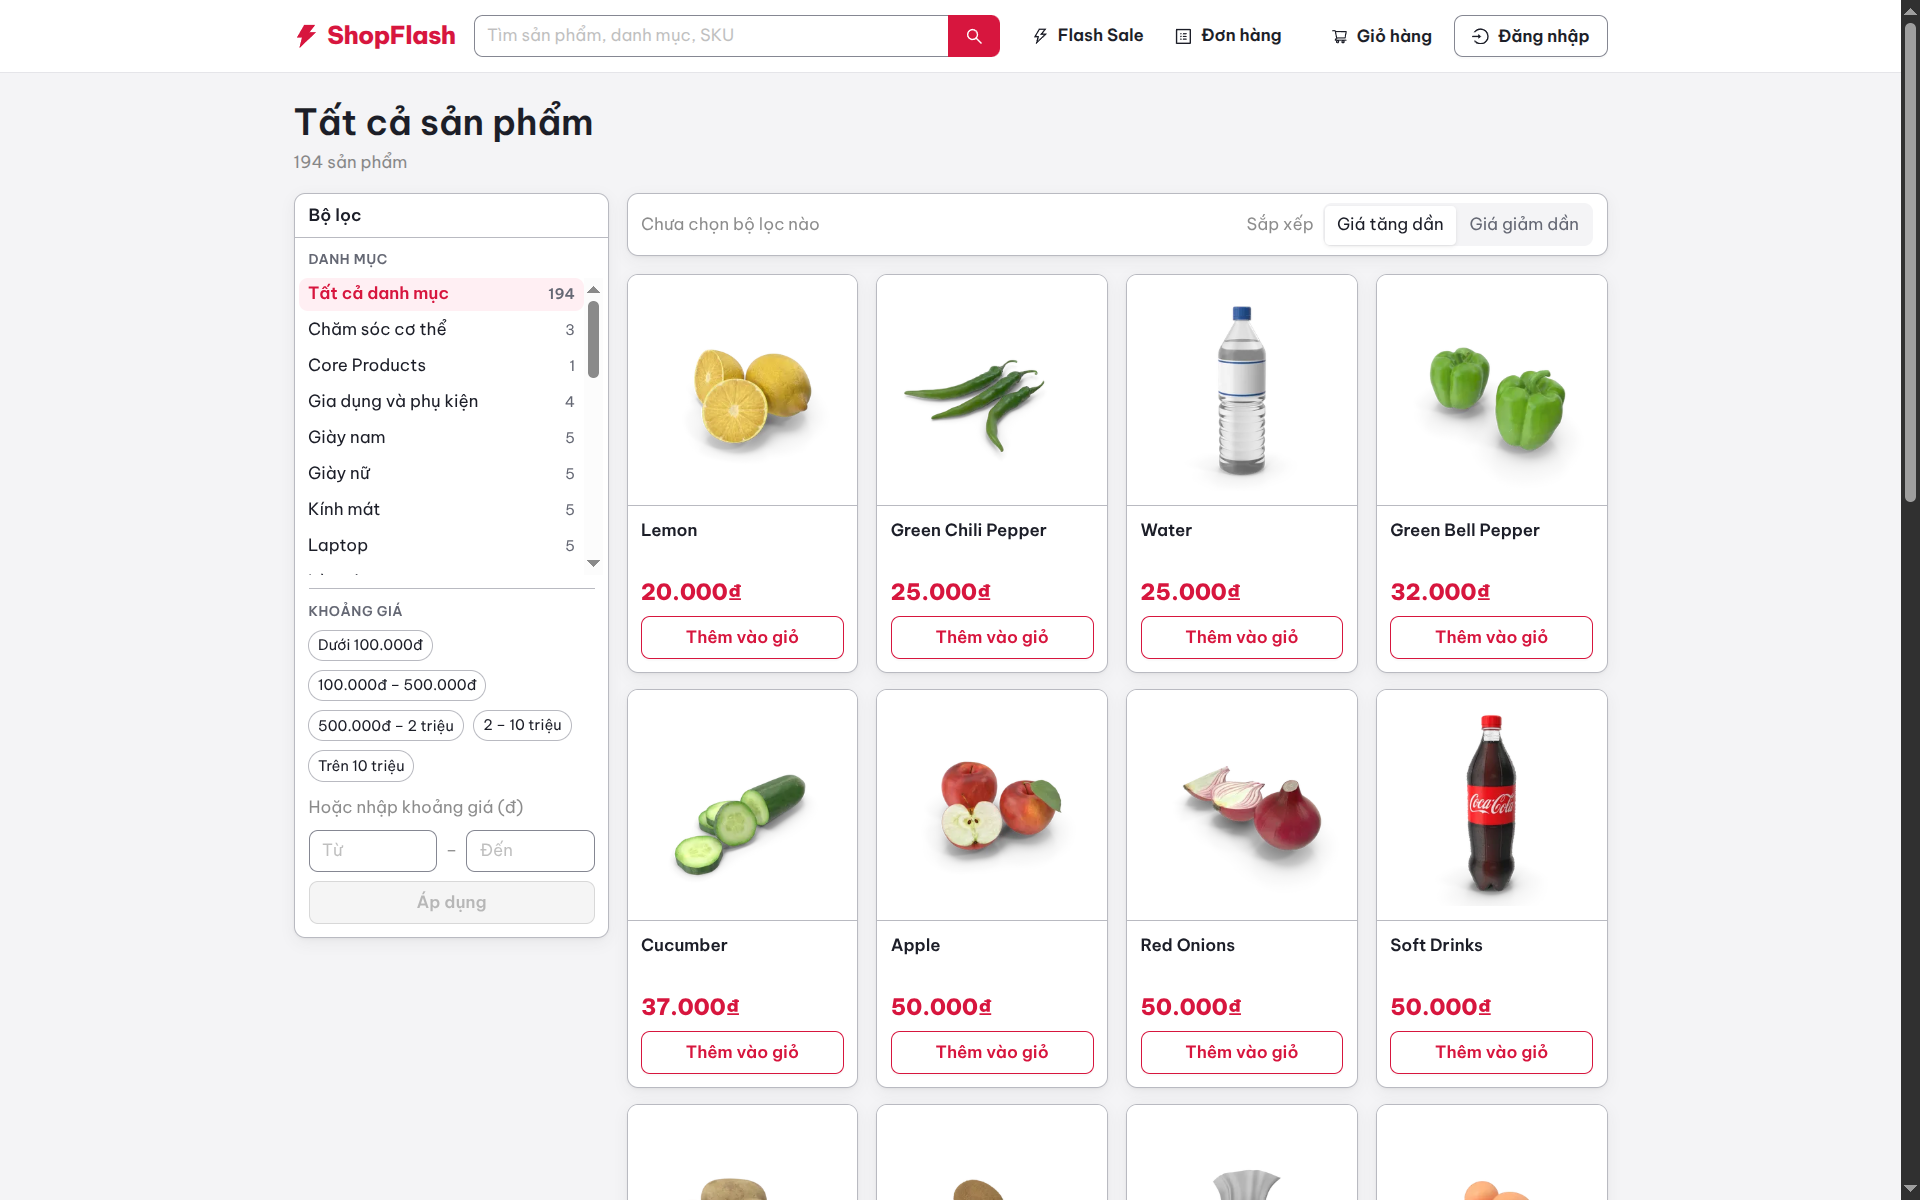
\includegraphics[width=\linewidth]{Pictures/Section_3/client-product-search.png}
\caption{Giao diện danh sách sản phẩm với bộ lọc và chức năng sắp xếp.}\label{fig:impl-client-product-search}
\end{figure}


Hai màn hình minh họa khả năng truy xuất và tổ chức dữ liệu sản phẩm phục vụ nhu cầu tìm kiếm. Những cơ chế đánh chỉ mục và xử lý truy vấn tương ứng được phân tích trong các topic Indexing và Query Processing.

\paragraph*{Nhóm chức năng giỏ hàng và xác nhận đặt hàng}

Giỏ hàng cho phép khách hàng thêm, xóa, điều chỉnh số lượng và lựa chọn những sản phẩm muốn đặt trong một lần Checkout. Hệ thống hiển thị giá trị từng dòng sản phẩm, tổng giá trị giỏ hàng và tổng tiền của những sản phẩm đã chọn.

Trong tình huống minh họa, giỏ hàng chứa năm dòng sản phẩm, trong đó khách hàng chọn ba dòng để đặt hàng với tổng giá trị \textbf{188.000 đồng}. Việc lựa chọn từng dòng giúp khách hàng chỉ mua một phần giỏ hàng mà không cần xóa các sản phẩm còn lại.

\begin{figure}[!htbp]
\centering
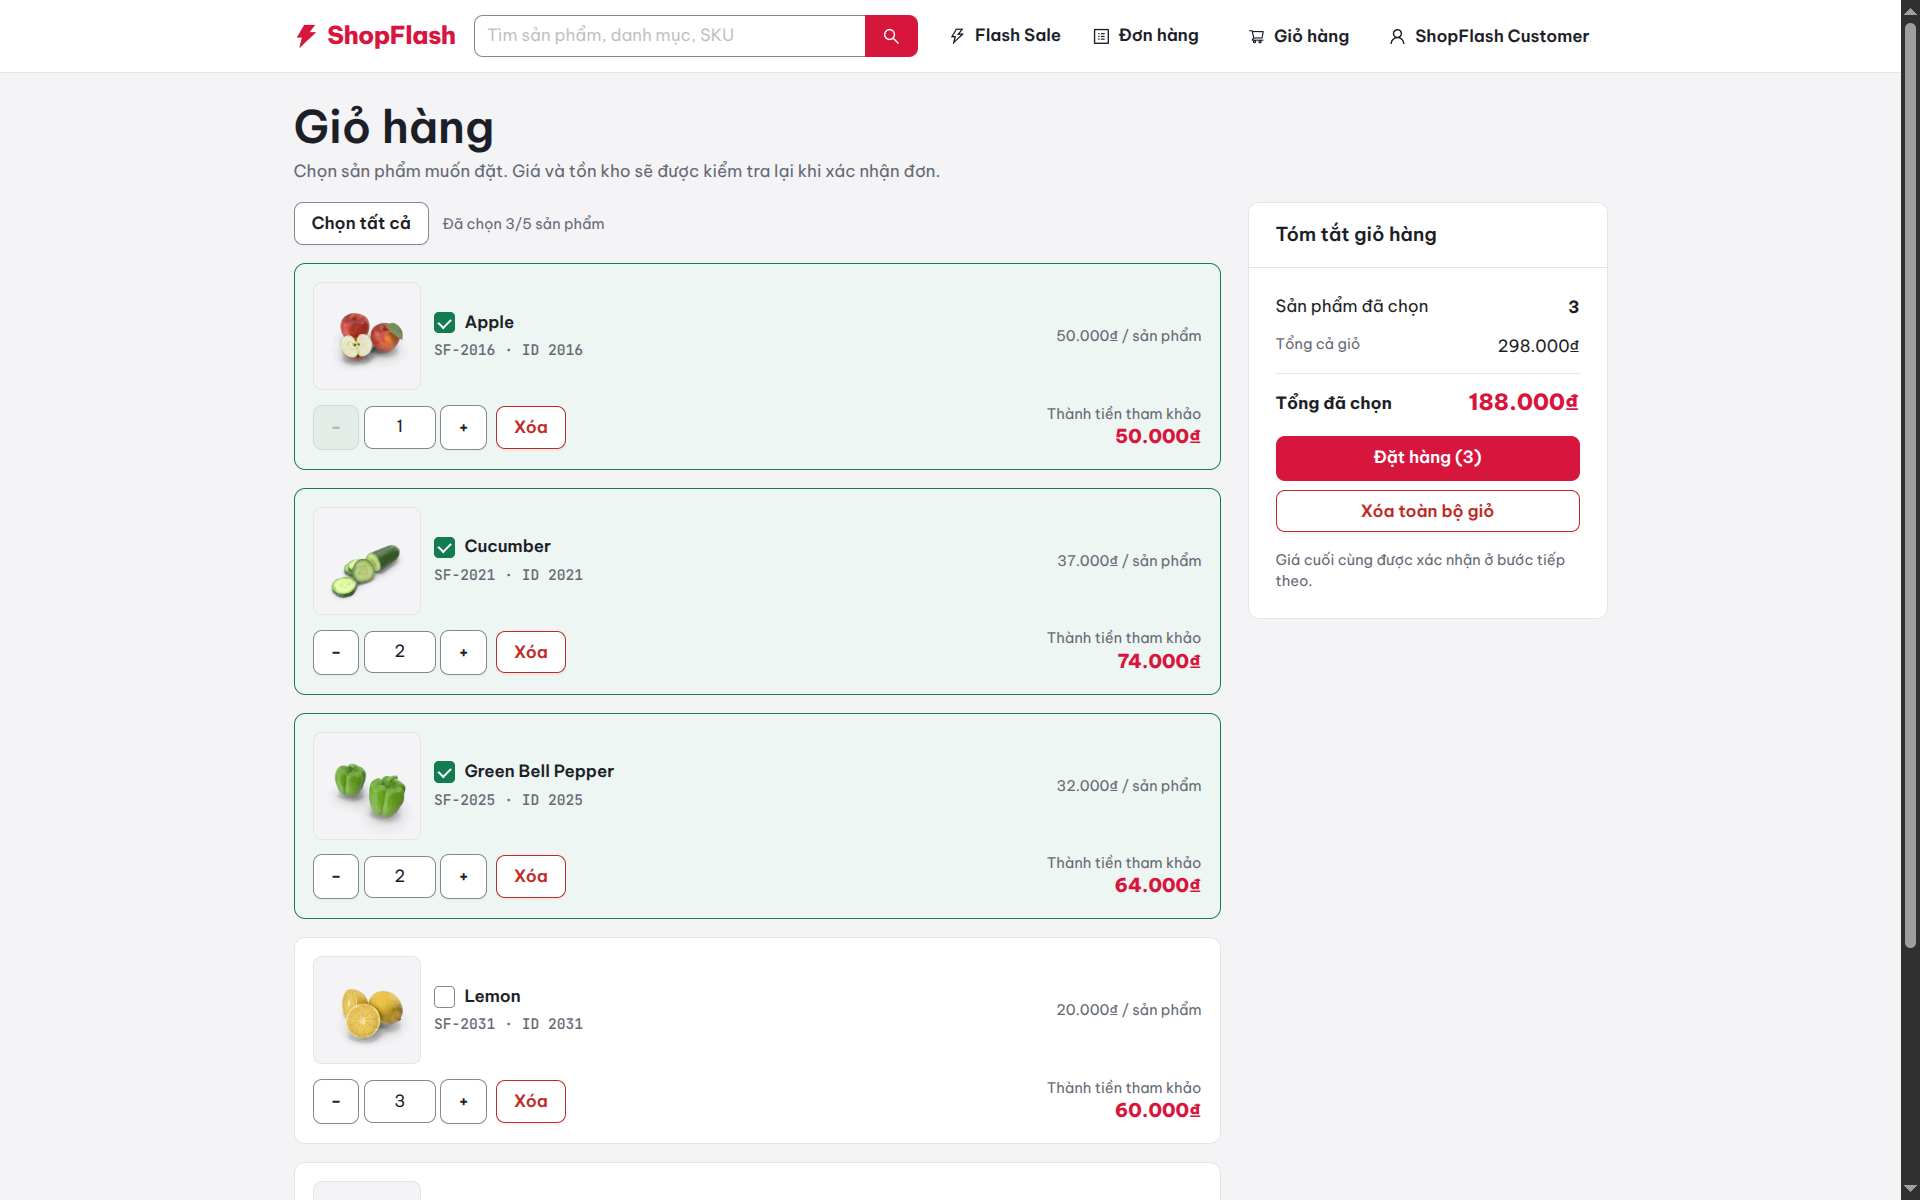
\includegraphics[width=\linewidth]{Pictures/Section_3/client-cart-selection.png}
\caption{Giao diện giỏ hàng, lựa chọn sản phẩm và tổng hợp giá trị đặt hàng.}\label{fig:impl-client-cart-selection}
\end{figure}


Sau khi chuyển đến bước Checkout, hệ thống hiển thị danh sách sản phẩm đã chọn, số lượng, thành tiền và thông tin nhận hàng. Khách hàng cung cấp tên, số điện thoại, địa chỉ giao hàng và kiểm tra lại đơn trước khi xác nhận.

Ở ví dụ này, đơn hàng gồm ba dòng sản phẩm: Apple (1), Cucumber (2) và Green Bell Pepper (2), với tổng tiền 188.000 đồng. Giao diện cũng hiển thị số lượng có thể bán của từng sản phẩm để người dùng tham khảo.

\begin{figure}[!htbp]
\centering
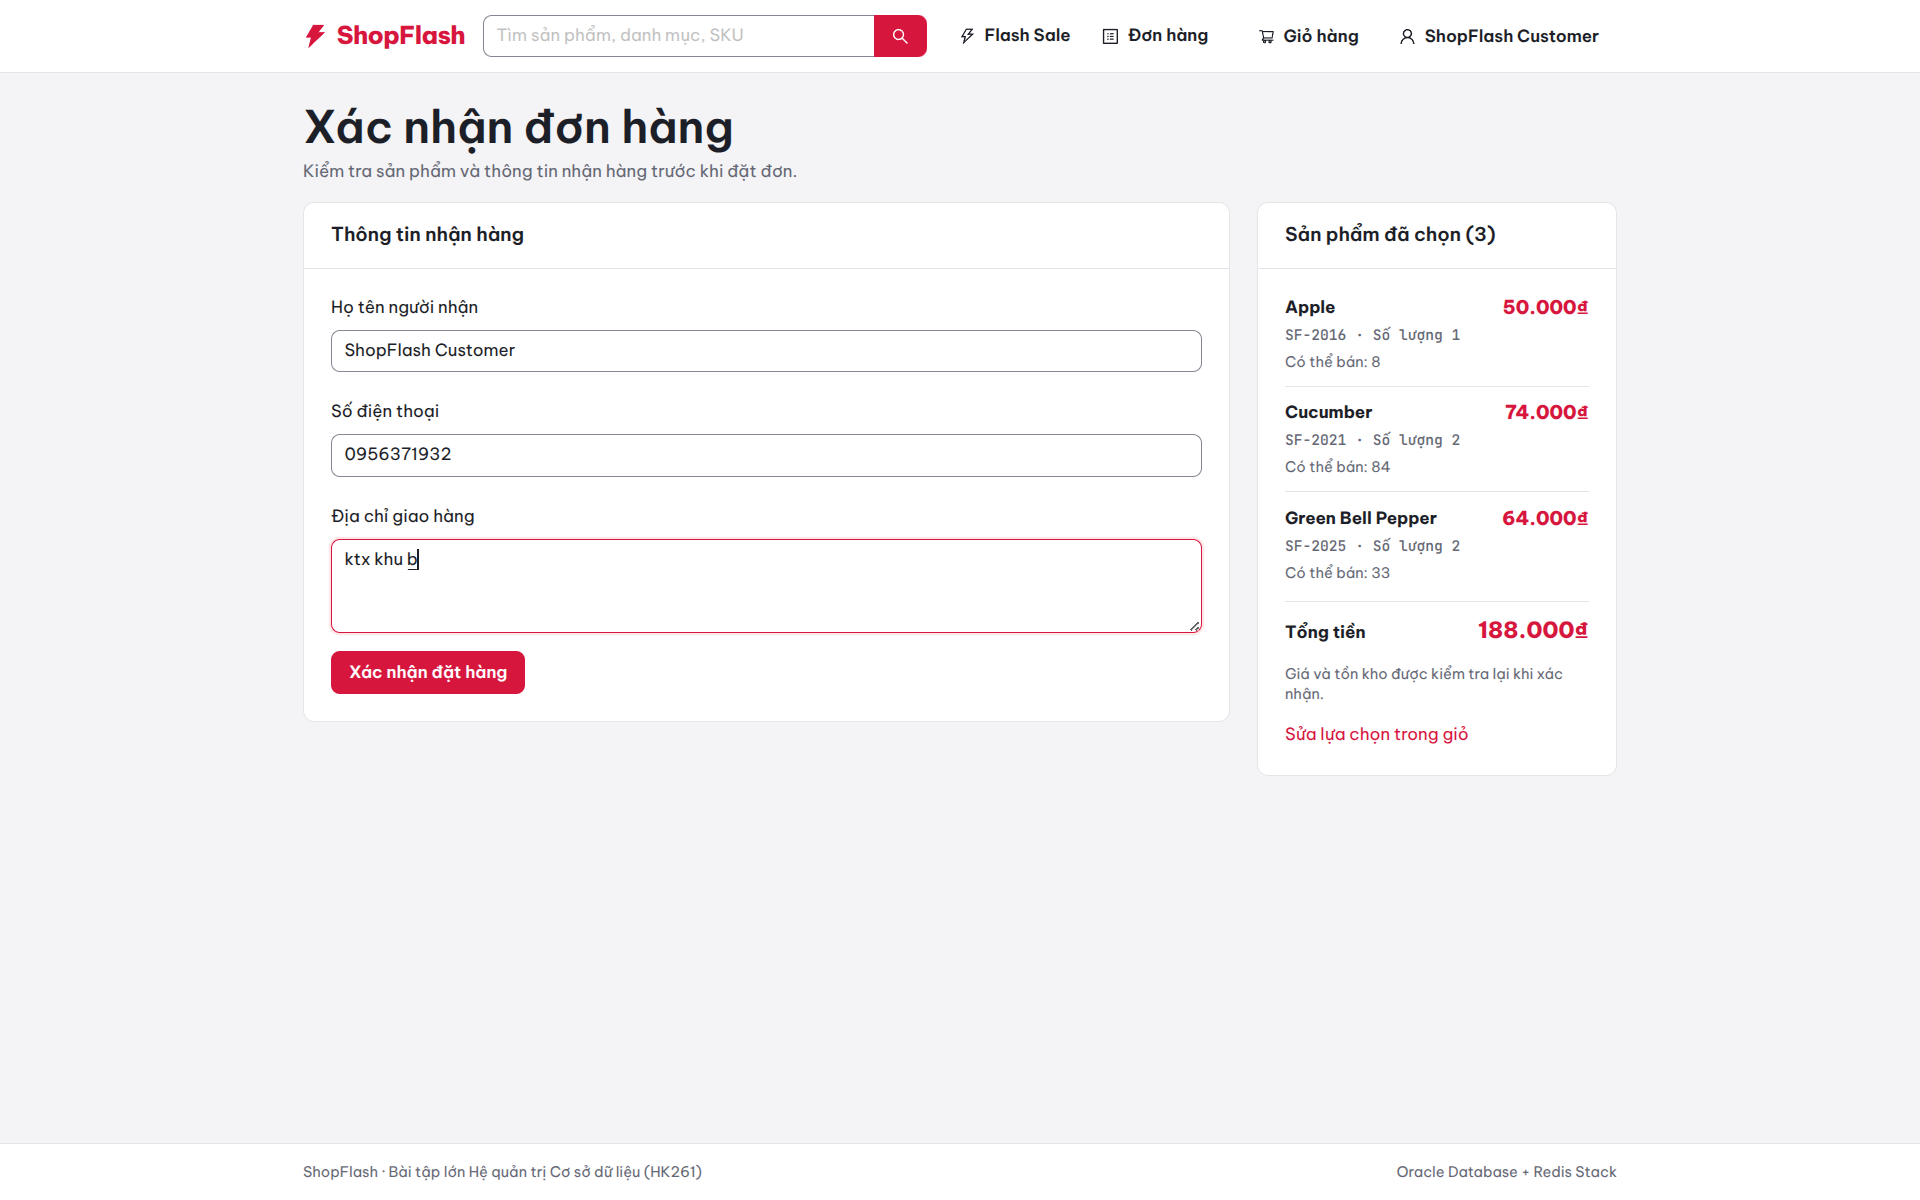
\includegraphics[width=\linewidth]{Pictures/Section_3/client-checkout.png}
\caption{Giao diện xác nhận đơn hàng với thông tin nhận hàng và danh sách sản phẩm.}\label{fig:impl-client-checkout}
\end{figure}


Thông tin giá và tồn kho được Backend kiểm tra lại khi người dùng xác nhận đặt hàng. Các thao tác tạo đơn, cập nhật tồn kho và giỏ hàng được quản lý trong Oracle transaction nhằm duy trì tính nhất quán của dữ liệu nghiệp vụ.

\paragraph*{Nhóm chức năng theo dõi và quản lý đơn hàng}

Sau khi đặt hàng, khách hàng có thể truy cập trang danh sách đơn để theo dõi những đơn đã tạo. Mỗi đơn được hiển thị với mã định danh, thời gian đặt, số lượng sản phẩm, tổng tiền và trạng thái xử lý.

Hình~\ref{fig:impl-client-orders} minh họa danh sách các đơn ở những trạng thái khác nhau, gồm Chờ xử lý, Đã xác nhận và Đã hoàn tất. Trong đó, đơn hàng mới có tổng giá trị \textbf{188.000 đồng}, gồm năm đơn vị sản phẩm và trạng thái \textbf{PENDING (Chờ xử lý)}.

\begin{figure}[!htbp]
\centering
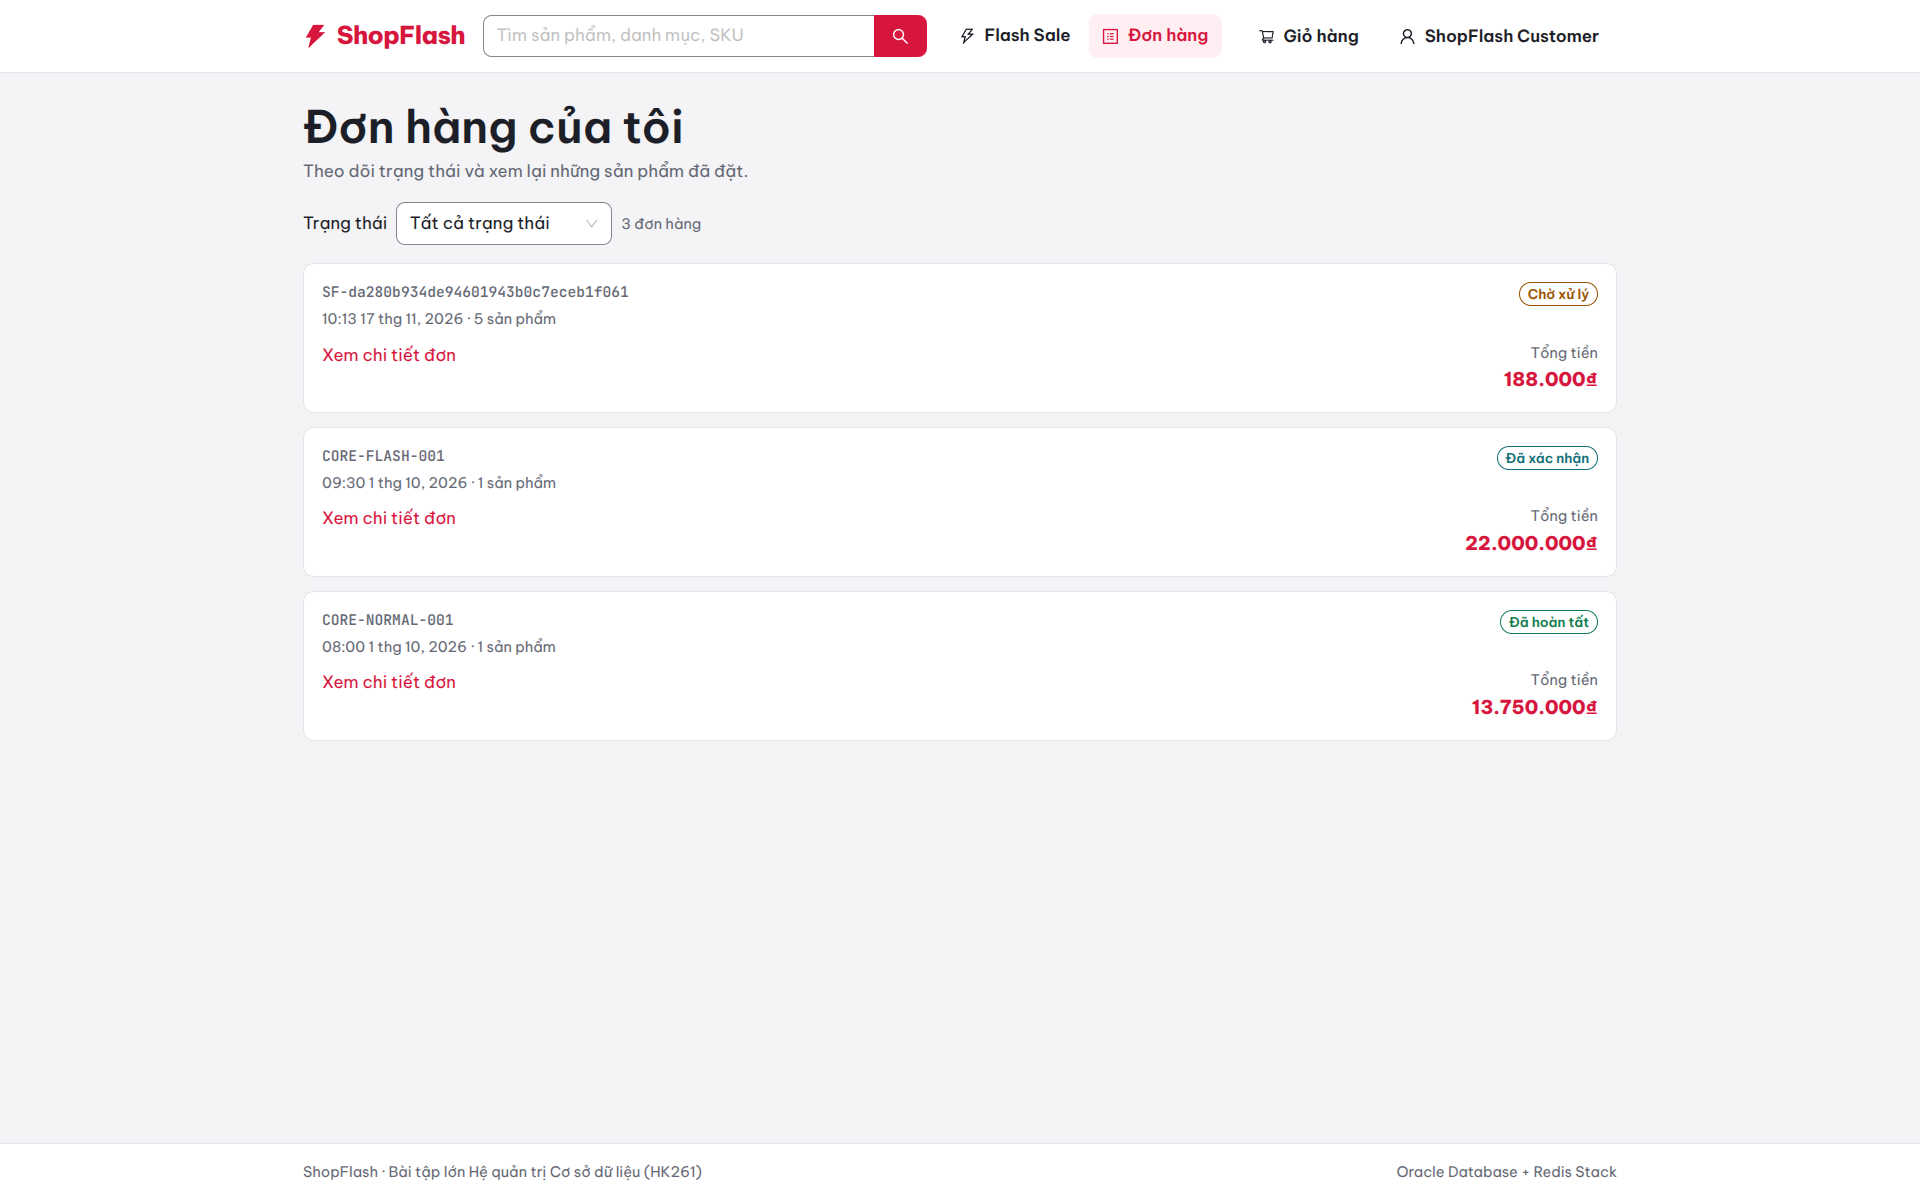
\includegraphics[width=\linewidth]{Pictures/Section_3/client-orders.png}
\caption{Giao diện danh sách đơn hàng và trạng thái xử lý.}\label{fig:impl-client-orders}
\end{figure}


Từ danh sách, người dùng có thể mở trang chi tiết để xem lại các sản phẩm đã mua, đơn giá, số lượng, thông tin nhận hàng và trạng thái đơn. Giá và thông tin sản phẩm được ghi nhận tại thời điểm đặt, giúp duy trì lịch sử đơn hàng ngay cả khi dữ liệu sản phẩm thay đổi về sau.

Hình~\ref{fig:impl-client-order-detail} thể hiện chi tiết đơn hàng vừa tạo, với ba dòng sản phẩm và tổng tiền 188.000 đồng, khớp với thông tin đã xác nhận tại bước Checkout. Đối với đơn hàng thông thường còn ở trạng thái PENDING, hệ thống cung cấp chức năng hủy đơn theo điều kiện nghiệp vụ.

\begin{figure}[!htbp]
\centering
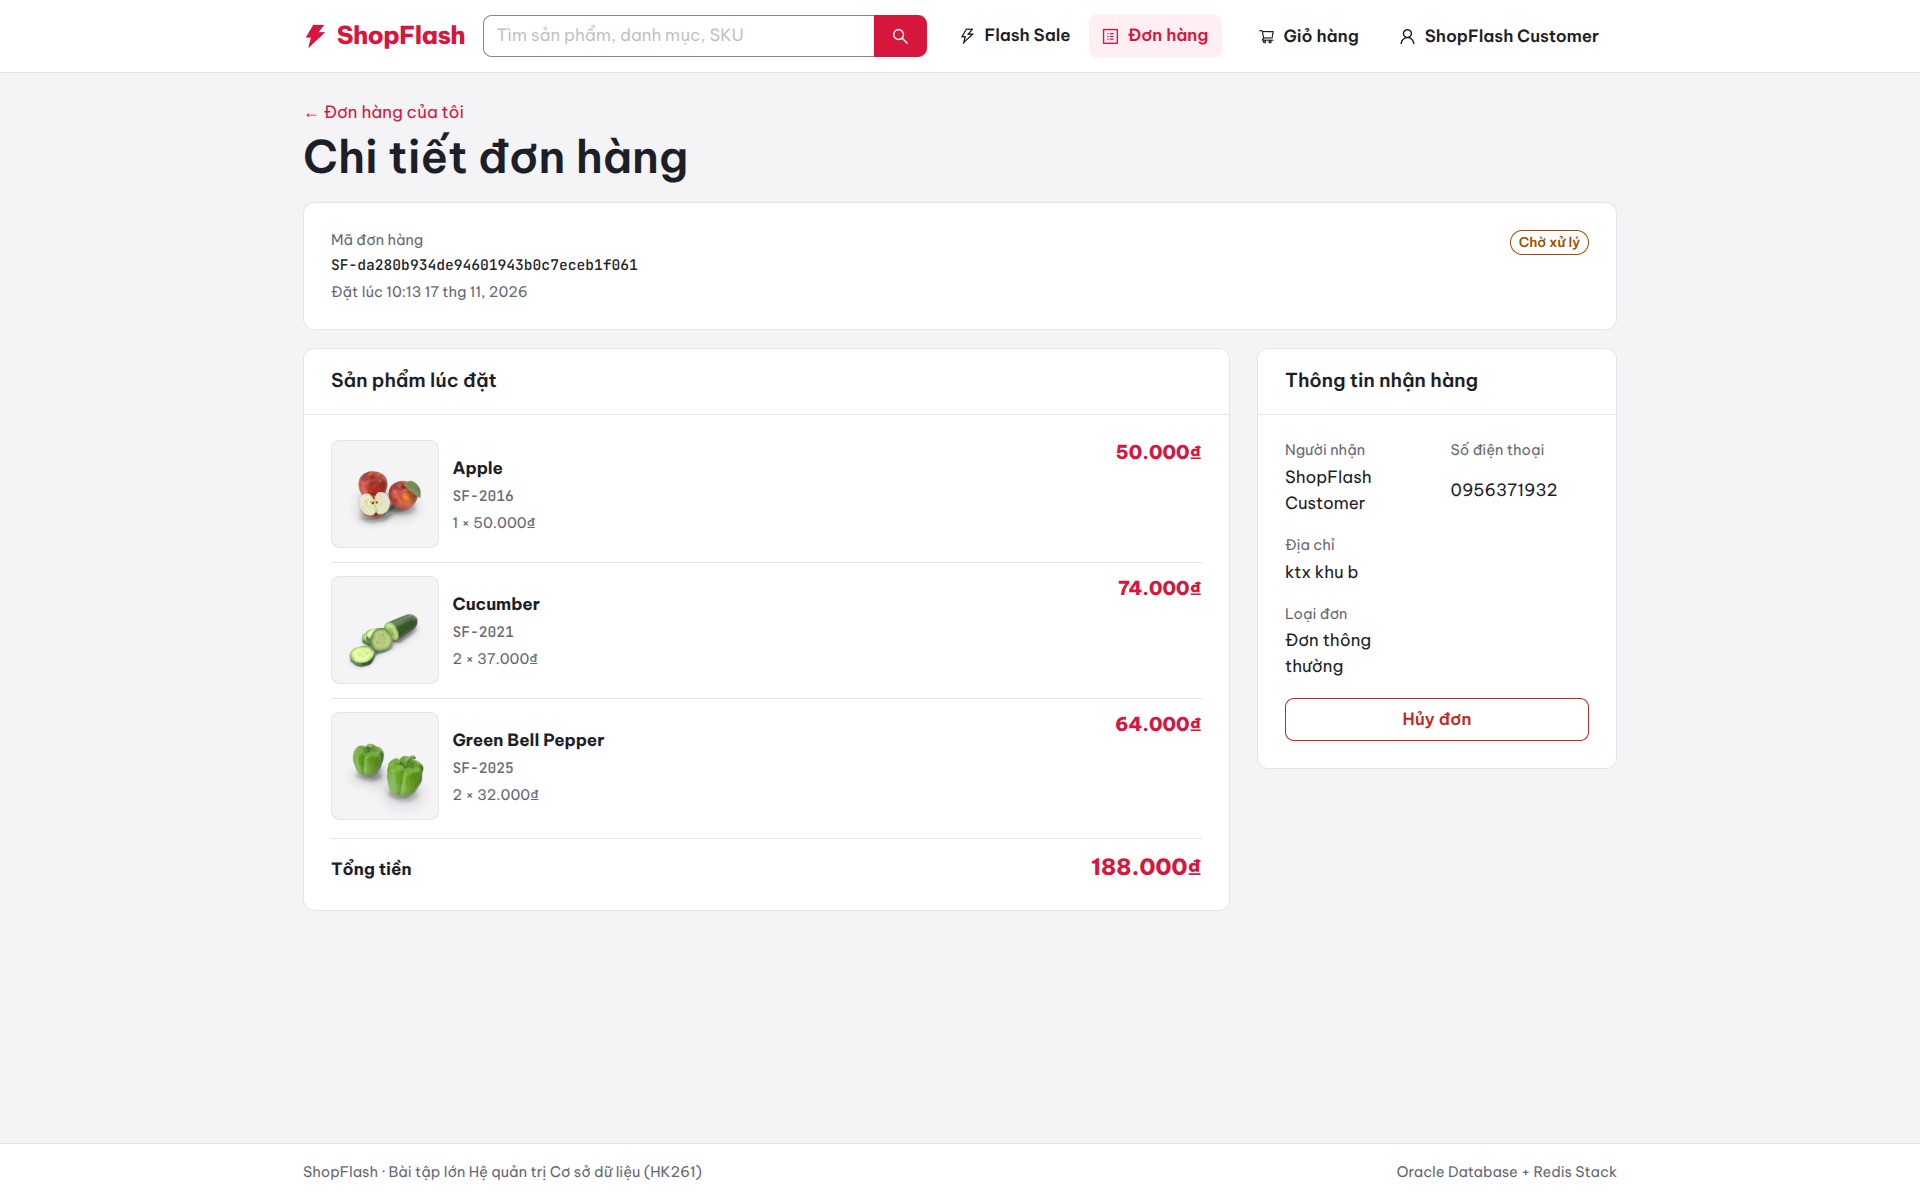
\includegraphics[width=\linewidth]{Pictures/Section_3/client-order-detail.png}
\caption{Giao diện chi tiết đơn hàng, sản phẩm đã mua và chức năng hủy đơn.}\label{fig:impl-client-order-detail}
\end{figure}


Nhóm màn hình này cho thấy luồng sử dụng liên tục từ giỏ hàng, xác nhận đặt hàng đến truy xuất đơn đã tạo. Các thông tin về số lượng và giá trị đơn được thể hiện nhất quán giữa những bước của giao diện.

\paragraph*{Nhóm chức năng Flash Sale}

Bên cạnh mua hàng thông thường, ShopFlash hỗ trợ các chương trình Flash Sale với số lượng sản phẩm được phân bổ giới hạn. Người dùng có thể xem sản phẩm đang tham gia chương trình, thực hiện giữ suất trong khoảng thời gian quy định và tiến hành đặt hàng.

Khác với Normal Checkout, luồng Flash Sale sử dụng Redis để quản lý quota và reservation tạm thời, trong khi Oracle lưu trữ đơn hàng và trạng thái nghiệp vụ chính thức. Chức năng này minh họa việc phối hợp hai DBMS trong bài toán mua hàng có cạnh tranh về số lượng.

Trang Flash Sale (Hình~\ref{fig:impl-client-flash-sale}) hiện các sản phẩm của chương trình đang mở bán với giá Flash Sale, số suất đã bán và còn lại; số suất được cập nhật mỗi 2 giây và đồng hồ đếm ngược chạy theo giờ của server.

\begin{figure}[!htbp]
\centering
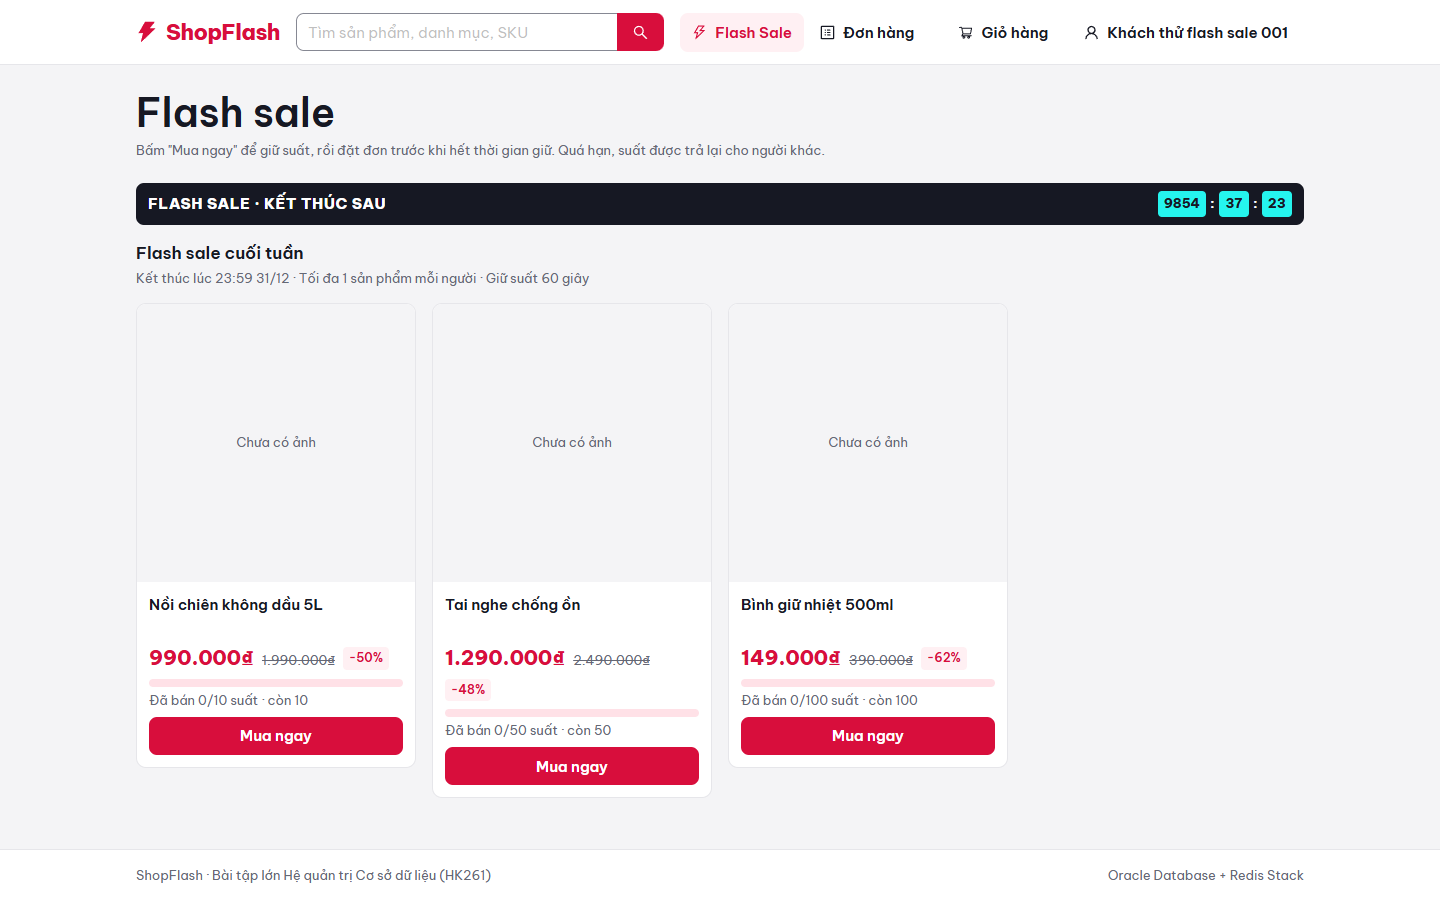
\includegraphics[width=\linewidth]{Pictures/Section_3/client-flash-sale.png}
\caption{Giao diện Flash Sale với số suất đã bán và còn lại của từng sản phẩm.}\label{fig:impl-client-flash-sale}
\end{figure}

Khi bấm ``Mua ngay'', khách giữ được một suất trong 60 giây và chuyển sang trang đặt đơn (Hình~\ref{fig:impl-client-flash-checkout}); nếu hết thời gian mà chưa đặt đơn, suất được trả lại cho người khác. Cơ chế giữ suất và kết quả thực nghiệm được trình bày ở mục~\ref{sec:cc}.

\begin{figure}[!htbp]
\centering
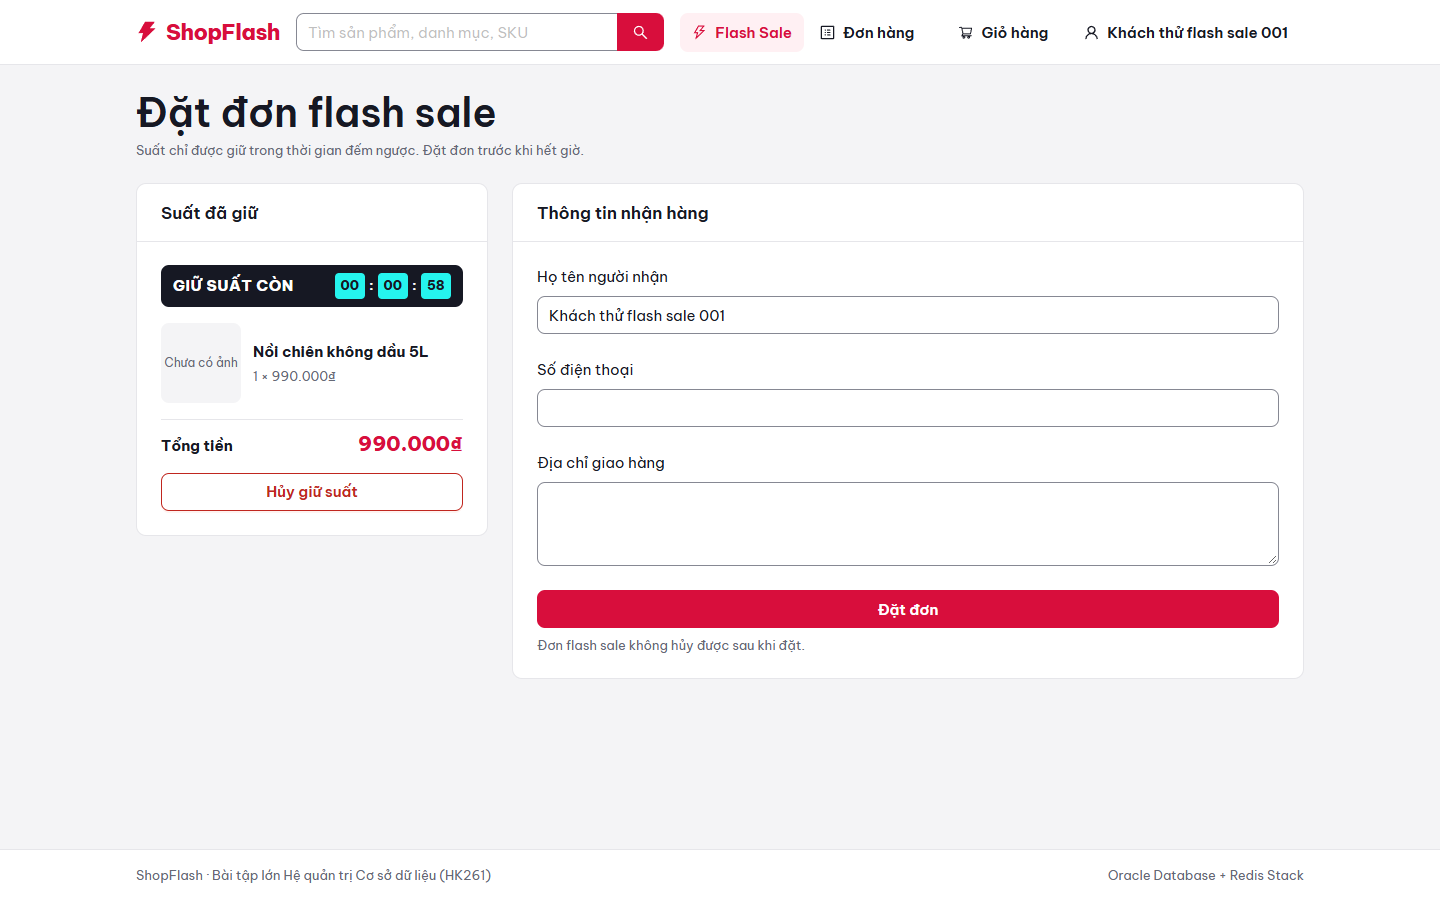
\includegraphics[width=\linewidth]{Pictures/Section_3/client-flash-checkout.png}
\caption{Giao diện đặt đơn Flash Sale trong thời gian giữ suất.}\label{fig:impl-client-flash-checkout}
\end{figure}

\subsubsection*{B. Giao diện phía quản trị (Admin)}

Ngoài các chức năng dành cho khách hàng, ShopFlash cung cấp giao diện quản trị nhằm quản lý dữ liệu và vận hành các nghiệp vụ của hệ thống. Phần này tập trung giới thiệu các nhóm chức năng tiêu biểu, không trình bày toàn bộ công cụ hỗ trợ thực nghiệm đã được phân tích tại Phần 2.

% Khung ảnh tạm: nếu chưa có file ảnh thì in ô chú thích thay vì làm hỏng bản dịch.
\newcommand{\adminfigure}[3]{%
\begin{figure}[!htbp]
\centering
\IfFileExists{Pictures/Section_3/#1.png}{\includegraphics[width=\linewidth]{Pictures/Section_3/#1.png}}{\fbox{\parbox{0.9\linewidth}{\centering [Chưa có ảnh #1.png]}}}
\caption{#2}\label{#3}
\end{figure}
}

\paragraph*{Nhóm chức năng quản lý danh mục và sản phẩm}

Quản trị viên quản lý danh mục tại trang Danh mục. Trang hiển thị danh sách phân trang gồm tên, mô tả, số sản phẩm và trạng thái của từng danh mục, hỗ trợ tìm kiếm theo tên, lọc theo trạng thái và thực hiện các thao tác tạo, sửa, xóa ngay trên trang.

\adminfigure{admin-categories}{Giao diện quản lý danh mục với tìm kiếm và lọc theo trạng thái.}{fig:impl-admin-categories}

Một danh mục chỉ được xóa khi không còn sản phẩm thuộc về nó. Giao diện vô hiệu hóa nút xóa đối với các danh mục còn sản phẩm (Hình~\ref{fig:impl-admin-categories}), đồng thời tầng xử lý nghiệp vụ vẫn kiểm tra lại quy tắc này để từ chối mọi yêu cầu xóa không hợp lệ.

\adminfigure{admin-products}{Giao diện quản lý sản phẩm với tìm kiếm, bộ lọc và phân trang.}{fig:impl-admin-products}

Form tạo và chỉnh sửa sản phẩm kiểm tra dữ liệu ngay khi nhập: danh mục, SKU, tên và giá bán là bắt buộc, giá không được âm. Khi tạo sản phẩm, hệ thống tạo luôn bản ghi tồn kho trong cùng một transaction. Sản phẩm không bị xóa cứng mà chuyển sang trạng thái ngừng bán để giữ nguyên lịch sử đơn hàng.

\adminfigure{admin-product-form}{Form tạo sản phẩm với kiểm tra dữ liệu đầu vào.}{fig:impl-admin-product-form}

Các màn hình này cho thấy dữ liệu danh mục và sản phẩm được lưu trên Oracle làm nguồn chính; sau mỗi thay đổi thành công, hệ thống cập nhật bản chiếu sản phẩm trên Redis để phục vụ tìm kiếm phía khách hàng. Cơ chế lưu trữ và so sánh giữa hai DBMS được phân tích tại topic Data Storage \& Management.

\paragraph*{Nhóm chức năng quản lý Flash Sale}

Quản trị viên tạo chương trình ở trạng thái nháp, chọn sản phẩm và số suất, rồi lên lịch. Khi lên lịch, hệ thống giữ trước hàng trong kho Oracle và nạp số suất lên Redis; chương trình tự chuyển sang đang chạy khi tới giờ và kết thúc sau giờ đóng. Danh sách chương trình hiện thời gian, trạng thái và số suất đã bán của từng chương trình (Hình~\ref{fig:impl-admin-flash-sales}). Trang chi tiết cho phép hủy lịch, hủy, dừng sớm, đối chiếu số liệu giữa Oracle và Redis, và dựng lại dữ liệu Redis từ Oracle (Hình~\ref{fig:cc-runtime}). Trang Concurrency Lab dùng cho thực nghiệm được trình bày ở mục~\ref{sec:cc}.

% Ảnh không có khung trình duyệt nên đặt hẹp hơn các ảnh Admin khác để cùng tỉ lệ chữ.
\begin{figure}[!htbp]
\centering
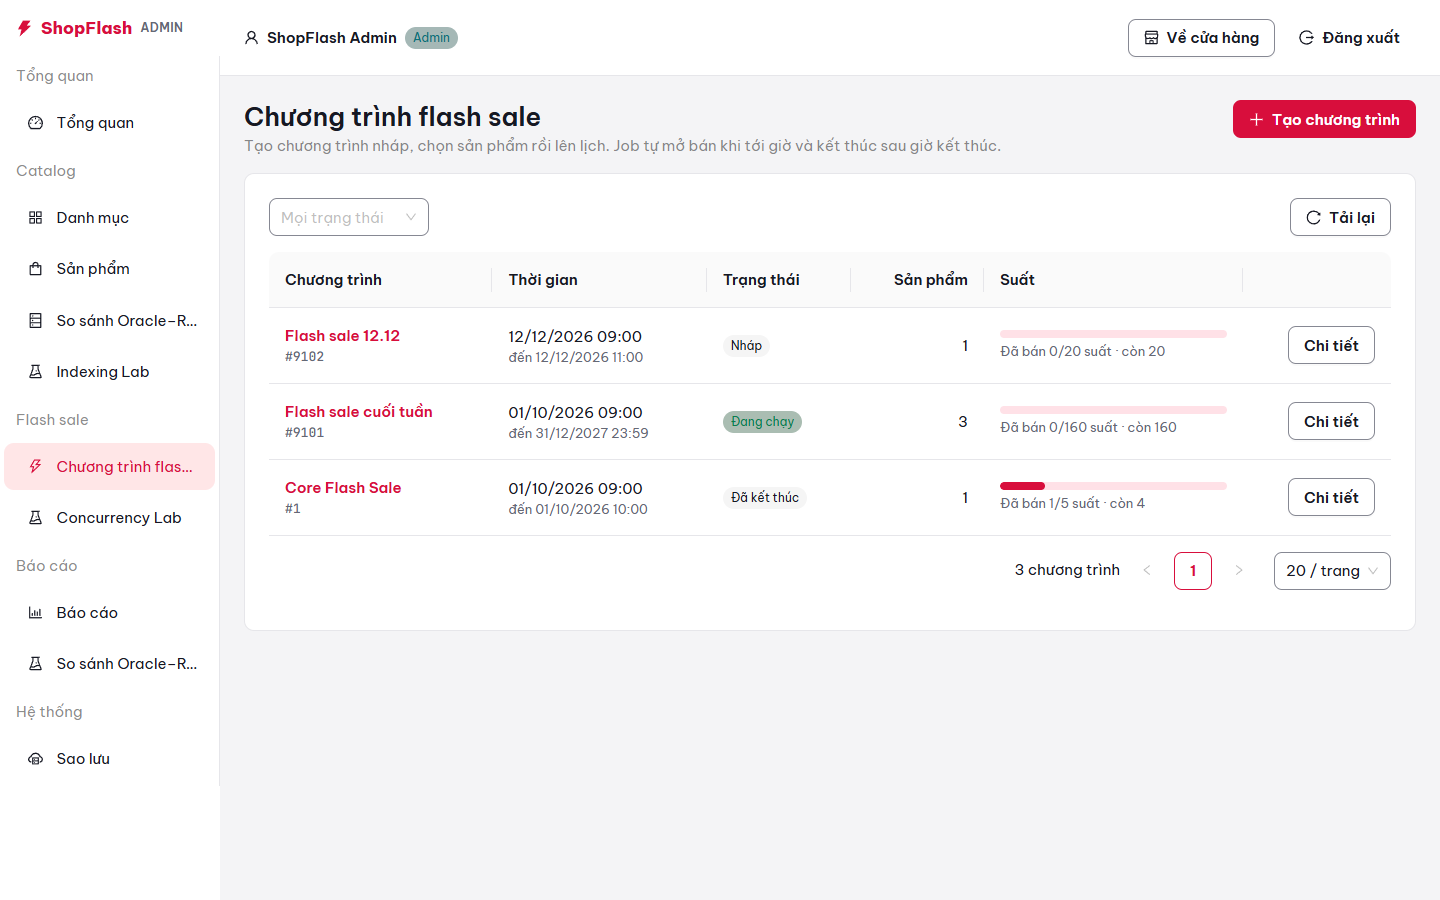
\includegraphics[width=0.72\linewidth]{Pictures/Section_3/admin-flash-sales.png}
\caption{Danh sách chương trình Flash Sale với trạng thái và số suất đã bán.}\label{fig:impl-admin-flash-sales}
\end{figure}

\subsubsection*{C. Đánh giá kết quả vận hành}

Các màn hình Client minh họa một luồng nghiệp vụ xuyên suốt, từ tìm kiếm sản phẩm, quản lý giỏ hàng đến đặt và theo dõi đơn hàng. Trong tình huống được trình bày, thông tin sản phẩm, số lượng và tổng tiền của đơn 188.000 đồng được thể hiện phù hợp giữa bước Checkout và trang chi tiết đơn hàng.

Ứng dụng cho phép người dùng thao tác thông qua React Frontend, thực hiện nghiệp vụ tại Spring Boot Backend và khai thác dữ liệu từ Oracle–Redis theo trách nhiệm đã thiết kế. Các ảnh giao diện là bằng chứng về kết quả hiển thị và khả năng tương tác; tính đúng đắn của cập nhật cơ sở dữ liệu và xử lý đồng thời được đánh giá thông qua các thí nghiệm, kiểm thử tương ứng tại Phần 2.

% Giữ phần kết luận ngắn cùng trang, tránh chỉ còn tiêu đề và đầu đoạn ở trang trước.
\clearpage
\subsection{Kết luận, hạn chế và hướng phát triển}\label{sec:conclusion}

\paragraph*{Kết quả đạt được}

Đề tài nghiên cứu và so sánh Oracle Database với Redis theo sáu chủ đề của môn học, kết hợp phân tích cơ chế, thực nghiệm và đánh giá trong bối cảnh ứng dụng thương mại điện tử ShopFlash. Kết quả của từng chủ đề cung cấp cơ sở để xác định những đặc điểm và phạm vi ứng dụng phù hợp của hai hệ quản trị.

Song song với nghiên cứu, nhóm đã xây dựng ứng dụng ShopFlash với các chức năng bán hàng, quản lý đơn hàng, Flash Sale và báo cáo thống kê. Hệ thống sử dụng Oracle làm nguồn dữ liệu nghiệp vụ chính, kết hợp Redis cho các tác vụ runtime, tìm kiếm và dữ liệu dẫn xuất.

\paragraph*{Hạn chế và hướng phát triển}

Phạm vi triển khai và kiểm chứng hiện tập trung vào môi trường local. Trong những giai đoạn tiếp theo, nhóm có thể mở rộng đánh giá trên các workload lớn hơn, tăng cường kiểm thử truy cập đồng thời, hoàn thiện cơ chế đồng bộ và phục hồi dữ liệu, cũng như khảo sát khả năng vận hành trong môi trường triển khai thực tế.

\paragraph*{Tự đánh giá}

Đề tài đáp ứng định hướng kết hợp nghiên cứu DBMS với xây dựng ứng dụng, cung cấp những tình huống nghiệp vụ cụ thể để kiểm chứng và lựa chọn các cơ chế quản lý dữ liệu. Những kết quả thu được có giá trị trong phạm vi mô hình và điều kiện thực nghiệm đã triển khai, đồng thời là cơ sở để tiếp tục phát triển hệ thống.

\par
\endgroup

% Chỉ hiện tài liệu tham khảo khi các phần nội dung có trích dẫn.
\ifreportcitations
  \clearpage
  \printbibliography[heading=bibintoc,title={Tài liệu tham khảo}]
\fi
\label{LastPage}
\end{document}
